% !TeX root = main.tex

%% This is the "preamble" of the document. This is where the format options get set.
%% Pro-tip: things following the % mark will not be compiled by LaTeX. I'll be using them extensively to explain things as we go.
%% Note: not to scare you off of LaTeX, but it's normal to have problems. And ya girl has been having some. I've included the copyright info at the bottom of the document from the guy who wrote this package, because his documentation doesn't entirely match how it's actually used. So this is a combination of his working preamble along with my added commentary or explanation. 
%%% 
%
%
%%\documentclass[man,12pt,floatsintext]{apa7}
%% Document class input explanation ________________
%% LaTeX files need to start with the document class, so it knows what it's using
%% - This file is using the apa7 document class, as it has a lot of the formatting built in
%% There are two sets of brackets in LaTeX, for each command (the things that start with the slash \ )
%% - The squiggle brackets {} are mandatory for executing the command
%% - The square brackets [] are options for that command. There can be more than one set of square brackets for some commands
%% Options used in this document (general note - for each of these, if you want to use the other options, swap it out in that spot in the square brackets):
%% - stu: this sets the `document mode' as the "student paper" version. Other options are jou (journal), man (manuscript, for journal submission), and doc (a plain document)
%% --- The student setting includes things like 'duedate', 'course', and 'professor' on the title page. If these aren't wanted/needed, use the 'man' setting. It also defaults to including the tables and figures at the end of the document. This can be changed by including the 'floatsintext' option, as I have for you. If the instructor wants those at the end, remove that from the square brackets.
%% --- The manuscript setting is roughly what you would use to submit to a journal, so uses 'date' instead of 'duedate', and doesn't include the 'course' or 'professor' info. As with 'stu', it defaults to putting the tables and figures at the end rather than in text. The same option will bump those images in text.
%% --- Journal ('jou') outputs something similar to a common journal format - double columned text and figurs in place. This can be fun, especially if you are sumbitting this as a writing sample in applications.
%% --- Document ('doc') outputs single columned, single spaced text with figures in place. Another option for producing a more polished looking document as a writing sample.
%% - 12pt: sets the font size to 12pt. Other options are 10pt or 11pt
%% - floatsintext: makes it so tables and figures will appear in text rather than at the end. Unforunately, not having this option set breaks the whole document, and I haven't been able to figure out why. IT's GREAT WHEN THINGS WORK LIKE THEY'RE SUPPOSED TO.
%
%\usepackage[american]{babel}
%
%\usepackage{csquotes} % One of the things you learn about LaTeX is at some level, it's like magic. The references weren't printing as they should without this line, and the guy who wrote the package included it, so here it is. Because LaTeX reasons.
%\usepackage[style=apa,sortcites=true,sorting=nyt,backend=biber]{biblatex}
%\addbibresource{references.bib} % This is the companion file to the main one you're writing. It contains all of the bibliographic info for your references. It's a little bit of a pain to get used to, but once you do, it's the best. Especially if you recycle references between papers. You only have 
%% biblatex: loads the package that will handle the bibliographic info. Other option is natbib, which allows for more customization
%% - style=apa: sets the reference format to use apa (albeit the 6th edition)
%\DeclareLanguageMapping{american}{american-apa} % Gotta make sure we're patriotic up in here. Seriously, though, there can be local variants to how citations are handled, this sets it to the American idiosyncrasies  to get the pieces in the holes once.`
%
%\usepackage[T1]{fontenc} 
%\usepackage{mathptmx} % This is the Times New Roman font, which was the norm back in my day. If you'd like to use a different font, the options are laid out here: https://www.overleaf.com/learn/latex/Font_typefaces
%% Alternately, you can comment out or delete these two commands and just use the Overleaf default font. So many choices!


%% Title page stuff _____________________
%\title{Some Title} % The big, long version of the title for the title page
%\shorttitle{Some Short title} % The short title for the header
%\author{Tejas Savalia}
%\date{\today}
%% \date{January 17, 2024} The student version doesn't use the \date command, for whatever reason
%\affiliation{UMass Amherst}
%%\course{PSY 4321} % LaTeX gets annoyed (i.e., throws a grumble-error) if this is blank, so I put something here. However, if your instructor will mark you off for this being on the title page, you can leave this entry blank (delete the PSY 4321, but leave the command), and just make peace with the error that will happen. It won't break the document.
%\professor{Dr. Professor}  % Same situation as for the course info. Some instructors want this, some absolutely don't and will take off points. So do what you gotta.
%
%\abstract{This is the abstract for this paper, wherein the main points of the introduction, method, results, and discussion are quickly talked about. Probably in more than one sentence, though. Dare I guess, more than two? There is a page break before starting the Introduction.}
%
%%\keywords{APA style, demonstration} % If you need to have keywords for your paper, delete the % at the start of this line
%
%\begin{document}
%\maketitle % This tells LaTeX to make the title page

% \section{Introduction} This command is commented out, because I was taught it was redundant to have the paper's title and introduction together. If your instructor wants it to say "Introduction", delete the % at the start


%% 
%% This is a sample doctoral dissertation.  It shows the appropriate
%% structure for your dissertation.  It should handle most of the
%% strange requirements imposed by the Grad school; like the different
%% handling of titles of one/many appendices.  It will automatically
%% handle the linespacing changes.  The body default is double-spaced
%% (except when you use the singlespace or condensed options).  The
%% default for quotations is single-space, and the default for tabular
%% environments is also single-space.  
%%
%% This class adds the following commands and environments to the
%% report class, upon which it is based:
%% Commands
%% ------------
%% \degree{name}{abbrv} -- Sets the name and abbreviation for the degree.
%%                         These default to ``Doctor of Philosopy''
%%                         and ``Ph.D.'', respectively.
%% \copyrightyear{year} -- for the copyright page.
%% \bachelors{degree}{institution} -- for the abstract
%% \masters{degree}{institution}   --  "
%%     if you have other degrees you may use
%% \secondbachelors{degree}{institution}
%% \thirdbachelors{degree}{institution}
%% \secondmasters{degree}{institution}
%% \thirdmasters{degree}{institution}
%% \priordoctorate{degree}{institution}
%%
%% \committeechair{name}           -- for the signature page
%% or, if you have two co-chairs:
%% \cochairs{first name}{second name}
%%
%% \firstreader{name}              --  "
%% \secondreader{name}             --  "
%% \thirdreader{name}              -- (optional)
%% \fourthreader{name}             --  "
%% \fifthreader{name}              --  "
%% \sixthreader{name}              --  "
%% \departmentchair{name}          -- for the signature page
%% \departmentname{name}           --  "
%%
%% \copyrightpage                  -- produces the copyright page
%% \signaturepage                  -- produces the signature page
%%
%% \frontmatter                    -- these are required in their various
%% \mainmatter                     -- appropriate locations
%% \backmatter                     --
%%
%% \unnumberedchapter[toc]{name}   -- like \chapter, except that it
%%                                    produces an unnumbered chapter;
%%                                    alternatively, like \chapter*,
%%                                    except that it lists the chapter
%%                                    in the table of contents.
%%
%% New environments:
%%   dedication  -- for the dedication
%%   abstract    -- for the abstract
%%
%% The thesis documentclass is built on top of the report document class.
%% It accepts all of the options that the report class accepts, plus the
%% following:
%%     doublespace -- the default, indicates double spacing as per U.Mass.
%%                    requirements.  You will need this when you do your
%%                    final copy.
%%     singlespace -- for earlier work, not acceptable to the Grad school
%%     condensed   -- for earlier work, not acceptable to the Grad school,
%%                    creates condensed versions of the frontmatter. 
%%                    Condensed implies singlespace.
%%     dissertation - the default, indicates that this document is a
%%                    dissertation.
%%     proposal    -- indicates that this document is a dissertation proposal,
%%                    rather than a dissertation.  This will only change the
%%                    wording on the title and signature pages.
%%     thesis      -- indicates that this document is a Master's thesis 
%%                    rather than a doctoral dissertation.  This also changes
%%                    the default for \degree to Master of Science, M.S.
%%     allowlisthypenation -- (the default), allows hyphenation of words in
%%                    the table of contents, the list of figures, and the list
%%                    of tables.  I believe that this is acceptable to the 
%%                    Graduate School.
%%     nolisthyphenation -- disallows hyphenation of words in the table of
%%                    contents and the list of figures and tables.  Use this 
%%                    option if the Grad School doesn't like your hyphenation.
%%     nicerdraft  -- relaxes some of the Grad School's rules for working with
%%                    drafts -- has no effect when doublespace is in effect
%%     nonicerdraft -- the default, leaves things in draft as they will be in
%%                     the final version
%% umassthesis changes the default font size to 12pt, but you may specify 10pt or
%%   11pt in the options.
\documentclass[dissertation]{umassthesis}          % for Ph.D. dissertation or proposal
% \documentclass[thesis]{umassthesis}  % for Master's thesis

%%
%% If you have enough figures or tables that you run out of space for their
%% numbers in the List of Tables or List of figures, you can use the following
%% command to adjust the space left for numbers.  The default is shown:
%%
%% \setlength{\tablenumberwidth}{2.3em}

%% Use the hyperref package if you're producing a version for online
%% distribution and you want hyperlinks.  Note that the Grad School doesn't want
%% their PDF viewers to colorize or otherwise highlight the links; use the
%% hidelinks option to hyperref to avoid decorating links.
%\usepackage[hidelinks]{hyperref}

%% One way of formatting the epigraph/frontispiece is to use this package.
%\usepackage{epigraph}
% \usepackage{biblatex}
\usepackage{amsmath}
\usepackage[hidelinks]{hyperref}
\usepackage{graphicx}
\usepackage{booktabs}
\usepackage{multirow}
% \usepackage{tikz}
% \usepackage{subcaption}


% \bibliographystyle{umassthesis}
%\usepackage{apa7}

\begin{document}
	
%%
%% You must fill in all of these appropriately
\title{Investigating the Role of Predictive Representations in Implicit Event Boundaries, Statistical Learning, and Categorization.}
\author{Tejas Savalia}
\date{September 2024} % The date you'll actually graduate -- must be
% February, May, or September
\copyrightyear{2024}
\bachelors{B.E.}{Gujarat Technological University}
\masters{M.S.}{International Institute of Information Technology, Hyderabad}
\secondmasters{M.S.}{University of Massachusetts Amherst}
%\priordoctorate{M.D.}{University of Never-never-land}
\committeechair{Andrew Cohen}
%\cochairs{B. B. Bahh}{I. M. A. Wolf}
\firstreader{Jeffrey Starns}
\secondreader{Youngbin Kwak}
\thirdreader{Meghan Huber}
%\fourthreader{}   % Optional
%\fifthreader{}            % Optional
%\sixthreader{}            % Optional
\departmentchair[Chair]{Maureen Perry-Jenkins} % Default uses "Department Chair" as the title. To
% use an alternate title, such as "Chair", use \departmentchair[Chair]{Pete Shearer}
% CICS uses "Chair of the Faculty" as of 2019.
\departmentname{Psychological and Brain Sciences}
% \departmentname{Robert and Donna Manning College of \\Information and Computer Sciences}


%% If your degree is something other than a Ph.D. (for a dissertation), or
%% an M.S. (for a thesis), you will need to uncomment the appropriate
%% following line:
%%
%% \degree{Doctor of Education}{Ed.D.}
%% \degree{Doctor of Philosophy}{Ph.D.}
%%
%% \degree{Master of Arts}{M.A.}
%% \degree{Master of Arts in Teaching}{M.A.T.}
%% \degree{Master of Business Administration}{M.B.A.}
%% \degree{Master of Education}{M.Ed.}
%% \degree{Master of Fine Arts}{M.F.A.}
%% \degree{Master of Landscape Architecture}{M.L.A.}
%% \degree{Master of Music}{M.M.}
%% \degree{Master of Public Administration}{M.P.A.}
%%\degree{Master of Public Health}{M.P.H.}
%% \degree{Master of Regional Planning}{M.R.P.}
%% \degree{Master of Science}{M.S.}
%% \degree{Master of Science in Accounting}{M.S. Acctg.}
%% \degree{Master of Science in Chemical Engineering}{M.S. Ch.E.}
%% \degree{Master of Science in Civil Engineering}{M.S.C.E.}
%% \degree{Master of Science in Electrical and Computer Engineering}{M.S.E.C.E.}
%% \degree{Master of Science in Engineering Management}{M.S. Eng. Mgt.}
%% \degree{Master of Science in Environmental Engineering}{M.S. Env. E.}
%% \degree{Master of Science in Industrial Engineering and Operations Research}{M.S.I.E.O.R.}
%% \degree{Master of Science in Manufacturing Engineering}{M.S. Mfg. Eng.}
%% \degree{Master of Science in Mechanical Engineering}{M.S.M.E.}
%%
%% \degree{Professional Master of Business Administration}{P.M.B.A.}


%%
%% These lines produce the title, copyright, and signature pages.
%% They are Mandatory; except that you could leave out the copyright page
%% if you were preparing an M.S. thesis instead of a PhD dissertation.
\frontmatter
\maketitle
\copyrightpage     %% not required for an M.S. thesis
\signaturepage

%%
%% Dedication is optional -- but this is how you create it
\begin{dedication}              % Dedication page
\begin{center}
	\emph{To those little lost sheep.}
\end{center}
\end{dedication}

%%
%% Epigraph (aka frontispiece) is also optional, but this is one way you
%% can create it
%\begin{frontispiece}
%  %% Format to your liking -- see documentation of epigraph package
%  \setlength{\epigraphrule}{0pt}
%
%  \begin{epigraphs}
%    \qitem{%
	%      \itshape
	%      Mary had a little lamb,\\
	%      Her fleece was white as snow.\\
	%      \vspace{\baselineskip}
	%      And everywhere that Mary went\\
	%      The lamb was sure to go.
	%      \vspace{\baselineskip}}
%    {Sarah Josepha Hale}
%
%    \vspace{2\baselineskip}
%    \qitem{%
	%      \itshape
	%      Baa, baa, black sheep,\\
	%      Have you any wool?\\
	%      Yes, sir, yes, sir,\\
	%      Three bags full;\\
	%      One for the master,\\
	%      And one for the dame,\\
	%      And one for the little boy\\
	%      Who lives down the lane.
	%      \vspace{\baselineskip}}
%    {English Nursery Rhyme}
%
%  \end{epigraphs}
%\end{frontispiece}

%%
%% Acknowledgements are optional...yeah, right.
\chapter{Acknowledgments}             % Acknowledgements page
Many people. 

%%
%% Abstract is MANDATORY. -- Except for MS theses
\begin{abstract}                % Abstract
We make sense of the world by extracting meaningful information from a continuous sensory stream. Extracting meaningful information involves first segmenting this continuous sensory stream into shorter, processable chunks. How do we algorithmically segment information into meaningful chunks? 

In this dissertation, I present an algorithmic predictive representational account of event segmentation. Maintaining a `context' representation where the context is defined by an expectation of upcoming future events naturally leads to separation of temporally disjoint events. I contrast this predictive account to an associative account and provide behavioral evidence in support for the predictive representational account. 

I then use the predictive representations as a common framework to understand cognitive processes of event cognition and categorization. Specifically, I first assess whether implicitly operationalized event boundaries (where changes in ongoing context that mark boundaries are not perceptually salient) provide the same behavioral properties as explicitly operationalized event boundaries thereby providing evidence for shared representations between the two. Finally, I apply the representation framework to understand the cognitive processes behind implicit category learning. I show that predictive representations can modulate category learning by providing on-going context information to items in each category.

Work in this dissertation thus advocates for predictive representations as a framework for understanding cognitive processes. In particular, if a cognitive process involves learning patterns, or summarizing information, I argue that predictive representations can serve as the common representational base upon which different operations lead to different cognitive processes. 

\end{abstract}

%%
%% Preface goes here...would be just like Acknowledgements -- optional
%% \chapter{Preface} 
%% ...


%%
%% Table of contents is mandatory, lists of tables and figures are 
%% mandatory if you have any tables or figures; must be in this order.
\tableofcontents                % Table of contents
\listoftables                   % List of Tables
\listoffigures                  % List of Figures

%%
%% We don't handle List of Abbreviations
%% We don't handle Glossary

%%%%%%%%%%%%%%%%%%%%%%%%%%%%%%%%%%%%%%%%%%%%%%%%%%%%%%%%%%%%%%%%%%%%%%%%%
%% Time for the body of the dissertation
\mainmatter   %% <-- This line is mandatory


\chapter{Introduction}
\label{introduction}
We experience a constant stream of sensory information from the moment we are born. Our brain parses this information and slowly learns to extract meaning from it. From recognizing the mother's scent as a survival instinct to formulating complex plans to defeat a board game opponent, our brain extracts meaning from our surroundings, considers prior experience and the current state of the world, and makes decisions to interact accordingly. My key question in this dissertation is: How do we learn to extract meaning from our surroundings?

Extracting meaningful information from our experience is beneficial to our functioning and survival. When approached by a cheetah in a forest, we do not wait to evaluate the exact number of spots on its skin before deciding to run. Such abstractions and formation of heuristics allow us to process naturally complex surroundings in quick time and act accordingly.

When extracting meaning from our surroundings, we often (need to) ignore minute details and abstract out towards a coherent thought of our surroundings. The extreme example above aside, we observe such abstractions in almost all day-to-day activities. Imagine someone asking you about the events during the day before reading this manuscript. Perhaps you are reading it on your office computer and you recall a sequence of events starting from waking up, to getting ready, driving or taking public transit to work, getting your morning coffee and breakfast in with an email check before turning your attention to this manuscript. Each event described above combines several sub-events that are abstracted away in such a verbal recall and description. For example, getting ready involves several steps from brushing your teeth, showering, and wearing your work outfits. Each sub-event can be further thought of as an abstraction from sub-sub-events -- brushing your teeth is a combination of putting toothpaste on the brush head, the physical act of brushing, followed by rinsing. While we perform each act continuously in time, our recall (and by extension, representation in memory) of these past events is discrete, segmented, and abstracted. The meaningfully separatable chunks of a continuous stream of events help in storage in (and retrieval from) memory.

There is often agreement on what it means for a chunk and for boundaries defining such chunks to be `meaningful'. In the example above, it is reasonable to argue that brushing teeth, showering, and putting on clothes are three distinct activities. Furthermore, even when the true transitions between these activities are continuous and seamless to a  independent, naive observer, the boundaries between these events are perceptually meaningful. What aspect of the environment dictates this agreement about the points at which we segment events and what is special about the properties of the events between those points that lead to distinct representations in memory?

One could argue that these events that occur at different points in time also occur at different spatial locations, thus providing different contexts and hence separate representations in our brain to be considered distinct. Transitioning from one (temporal) event to another can thus be akin to transitioning from one room of the house to another. However, it is almost impossible to decouple temporal events from spatial events assuming a causality from spatial segmentation to temporal segmentation for any spatially experienced distinct event is also a temporally experienced distinct event. Instead, arguing that temporally distinct events lead to a spatially distinct representation can provide a more encompassing explanation of distinct representations for events in distinct spatial \emph{and} temporal contexts. One could similarly argue that the formation of ``meaningful'' chunks is through perceptual differences between the events we experience. While lower-level perceptual experiences are indeed often different for different events, the mapping of perceptual differences onto segmented events is arbitrary and not a \emph{sufficient} condition. For example, eating an apple is recalled as eating an apple regardless of whether it has a green leaf added to its top. Perceptual distinctions are not enough to determine whether events are represented distinctly. What then is the key mechanism that leads to events being segmented? 

In this dissertation, I argue that the primary reason and mechanism through which we segment events is based on temporal contingencies of various sub-events that encompass an event. Specifically, we recall being in the kitchen as different from being in the bedroom because we have a coherent set of experiences in the kitchen that are distinct from a coherent set of experiences in the bedroom. For an infant forming knowledge of the world, a kitchen while perceptually distinct from a bedroom, is not meaningfully different. With experience and observation of the functions within these spatially (and perceptually) distinct locations, the child slowly develops distinct representations of the two rooms.

This dissertation focuses on understanding temporal contingencies' role in event segmentation, and by extension, general pattern extraction. I argue that even \emph{without} any spatial or perceptual information that may aid us in separating events in memory, we can use temporal coherence to experience separate events and abstract information to aid higher-level cognition. Specifically, I investigate the parsing of a continuous stream of information into discrete chunks in three ways:



\begin{itemize}
	\item
	The possible algorithmic processes that naturally lead to such segmentation and the impact of environmental properties in aiding this abstraction.
	\item
	The properties of the temporal boundaries when such temporal abstraction occurs naturally and implicitly.
	\item
	The role of temporal events separated by implicit temporal boundaries in forming abstractions.
\end{itemize}

\section{Scope of this dissertation}\label{scope-of-this-dissertation}

The human brain is a complex machine -- millions of neurons act as computational units and combine in specific ways to form a functioning human being. These neurons come together to implement several levels of function from lower-level automatic perception to higher-level planning and conscious thought. This dissertation does \textbf{not} focus on these implementational-level mechanisms of cognition. Rather, it focuses on \emph{algorithmic} computations that neurons may, collectively, implement that lead to us acquiring patterns in the environment around us.

Analyses in this dissertation use several models of cognition in investigating the role of implicit statistical learning. In most cases, the focus of this dissertation is \textbf{not} to evaluate the validity of these models. Indeed, most models of cognition are wrong; but are useful and I use several such models to evaluate specific aspects of how we acquire patterns. 

\section{Format of this dissertation}\label{format-of-this-dissertation}

In the rest of this dissertation, I present three lines of studies investigating the role of implicit temporal boundaries in cognition. In Chapter 2, I present an algorithmic framework that naturally leads to a representation of separable events without the need to rely on explicit properties of the experienced events. I also show that this framework allows for a distinct representation of event boundaries as special events. In Chapter 3, I present work comparing the properties of these event boundaries which are operationalized implicitly (i.e.~through no perceptually special information) with event boundaries as they have been studied in prior literature which are operationalized explicitly. Finally, in Chapter 4, I present work investigating the role of these implicitly operationalized event boundaries in categorization to serve as a gateway for understanding higher-order cognition in the context of temporal segmentation and pattern acquisition.earned.


\newpage

\chapter{Quality of Environmental Exposure modulates statistical learning}
\label{chapter-2-walk-lengths-modulate-statistical-learning}
\section{Introduction}

Imagine you just moved to the United States and are visiting Target for the first time. Perhaps since you just moved in, your first goal is to furnish your apartment. You look around at the entrance, and navigate your way to the furniture section perhaps while taking a few false turns on the way, buy the stuff you need, pay and leave. The next time you visit for, for example, groceries and produce. You visit again for sporting goods and then again for gifts for your friends. An year later, all such subset of visits through the Target store makes you an expert in knowing the specific route to the section you need to visit. What algorithmic mechanisms allow us to build such expertise to create connections in an explored environment even when during no single visit, you explored all possible connections between regions of the store?

We are able to build up a map of the environment without being exposed to the full extent of it in a single iteration simply based on local exposures to it. Such building is often implicit -- you just know that in order to go to the furniture area, you need to pass through the gifts even when you did not explicitly explore this connection before. In this chapter I explore some algorithmic mechanisms that may lead to our ability to acquire large-scale structural knowledge of the environment based on local exposures. 

The effect of local exposure in acquiring structural knowledge of the environment have been explored in several areas of cognitive psychology through artificial grammar and language learning \cite{knowlton1992intact, romberg2010statistical, aslin2012statistical, dehaene2015neural}, visual statistical learning \cite{fiser2002statistical, turk2008multidimensional, brady2008statistical}, or motor sequence learning \cite{baldwin2008segmenting, nissen1987attentional, cleeremans1991learning, kahn2018network}. In recent work, (implicit) acquisition of higher order knowledge of the environment from lower order exposure is studied through structured graph based transitions between stimuli \cite{schapiro2013neural, karuza2017process, kahn2018network, lynn2020humans, lynn2020human, karuza2022value}. For example \cite{schapiro2013neural} show that when asked to respond to arbitrary stimuli arranged in a temporally graph-modular structure, participants often parse the edges that connect two modules as `natural breaks' even when their local exposure does not distinguish between the cross-module and within-module edges. 

More commonly, global-scale structure acquisition has been attributed to response time measurements. Earlier work in serial reaction time tasks \cite{nissen1987attentional, cleeremans1991learning} shows that breaking an implicitly learned motor sequence leads to slower reaction times. The slowed reaction times when crossing the between-module edges have also been shown in recent work on statistical learning in modular graph structures \cite{kahn2018network, lynn2020humans, karuza2017process, karuza2022value, karuza2019human, lynn2020human}. 

This slowdown across module edges appears to be mediated by the nature of the walk experienced across the community structure where random and Eulerian walk (a walk where each edge of the graph is visited exactly once before repeats) experiences continue to show this slowdown whereas a Hamiltonian walk (a walk were each node of the graph is visited exactly once before repeats) experience does not \cite{karuza2017process}. Thus it appears that the kind of experience through the graph alters the knowledge of underlying statistical patterns. Similarly, the topographical structure of a graph in motor skill learning tasks also appears to alter structural knowledge \cite{lynn2020abstract, lynn2020human, lynn2020humans} where modular graphs like in Figure \ref{fig:modular_graph} produce the largest dip in reaction times when responding to boundary items.

\begin{figure}[ht]
	\centering
	\caption{Modular graph structure used in \cite{schapiro2013neural}. Locally, each node is connected to four nodes with each edge equally probable. However, globally, the graph structure consists of three sub-modules interconnected through `boundary nodes'}
	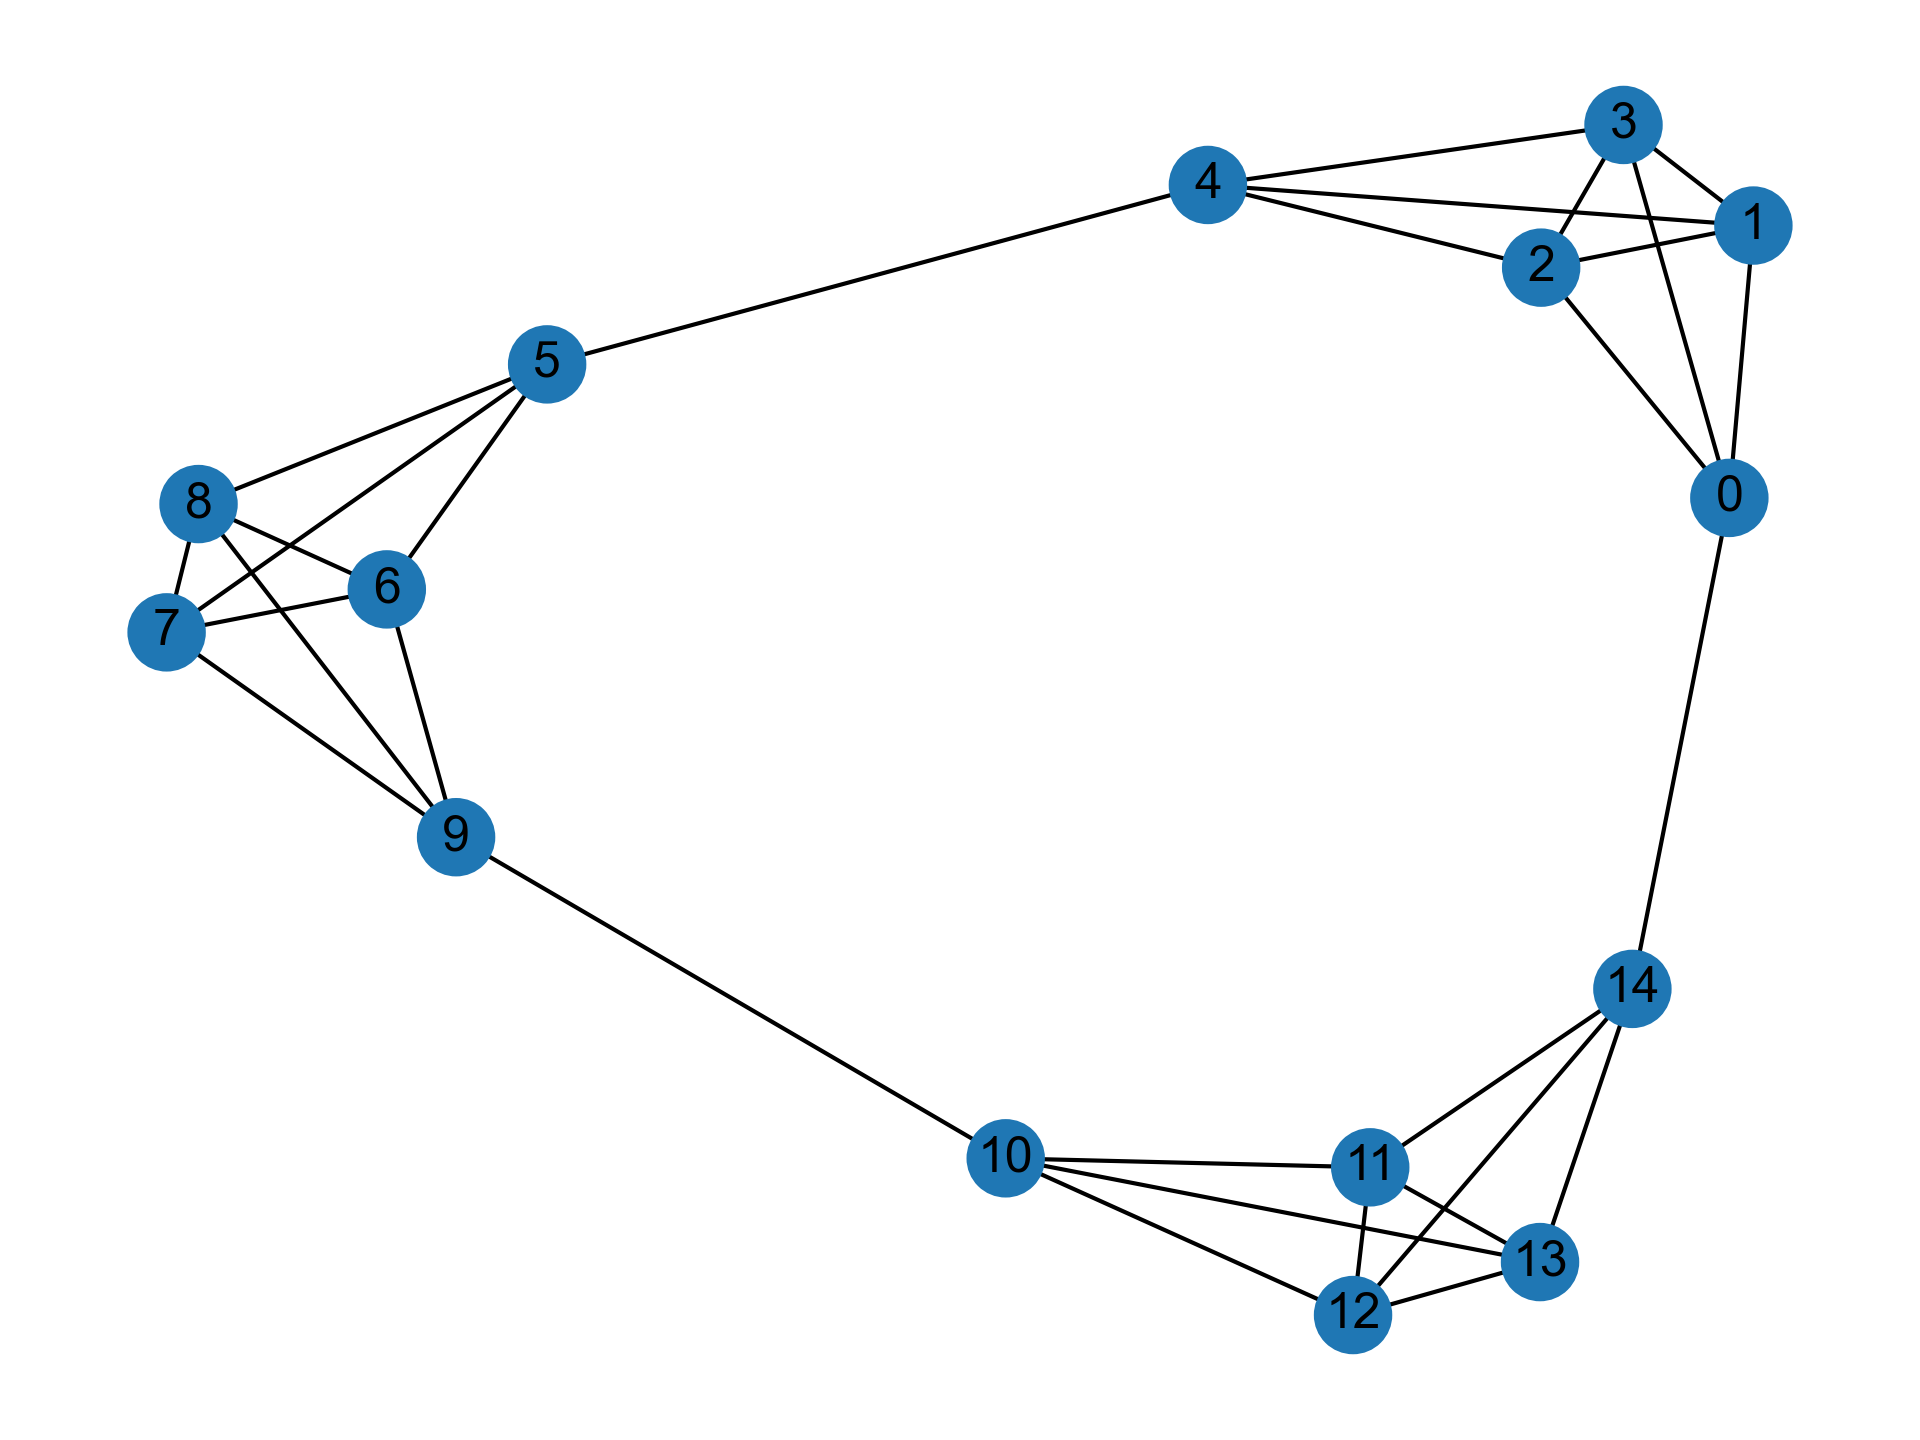
\includegraphics[width = \textwidth]{chapter_notebooks/chapter_2/figures/modular_graph.png}
	\label{fig:modular_graph}
\end{figure}

Why do we slow down at boundary nodes that lead to the adjacent module even when the local probability of that particular transition is the same as any other transitions? Understanding this particular property of human behavior may provide deeper insights into what leads to global-scale structure acquisition; after all the only difference between the boundary node and other non-boundary nodes is in context of the global structure of the graph. Event boundary literature (where boundaries are typically operationalized through explicit changes in context) suggests that boundaries alter the predictability of future events and this predictability leads to event segmentation \cite{zacks2007event, clewett2019transcending}. Thus, in implicitly operationalized boundaries such as in serial reaction time tasks, the slowdown at the boundary node may imply a similarly increased uncertainty at boundary nodes leading to slowed responses. Prior work aimed at understanding human representation of graph structures indeed points to an the `cross-entropy' between a learner's estimate of the transition probability and the true transition probability of the environment \cite{lynn2020abstract, lynn2020humans, lynn2020human}. 

%In addition to being uncertain about the immediate next stimulus, participants are also uncertain about switching to a neighboring cluster or staying within the same cluster.

In particular, \cite{lynn2020human} show that algorithms of contextual representations such as the Successor Representation (SR) model in Reinforcement Learning \cite{dayan1993improving, momennejad2017successor, gershman2018successor} or the associative learning based Temporal Context Model (TCM) can naturally lead to an increased cross-entropy for cross cluster transitions relative to within cluster transitions in modular graphs. In this work, by using the framework of cross-entropy to estimate reaction times in a modular graph we aim to 1) Experimentally test the predictions of these two models when exposure through the modular graph structure of is partial and 2) Provide evidence in favor of one of the two models of representation. 

\subsection{Representations of Temporal Context}

\subsubsection{Successor Representation}\label{successor-representation}

The Successor Representation (SR) model of reinforcement learning has been used as a model to understand the generalization of reinforcement learning behavior in large action spaces \cite{dayan1993improving}. In recent work, the SR model has also been shown to be a reliable model for explaining human decision-making behavior in multi-step environments. The model accurately predicted that humans are worse at adapting to changes in the transition probability of a learned environment than to changes in the end-point rewards \cite{momennejad2017successor}. There has been further evidence of SR being represented in the Hippocampal cells which represent space \cite{gershman2018successor, stachenfeld2017hippocampus}.

Briefly, the SR model represents each state in the actionable space as a predictive representation matrix. For an environment of $N$ discrete states, the SR matrix $M$ of size $(N X N)$ maintains expected future visits to a given state from each state. Specifically, element $M_{i,j}$ of the matrix represents the expected future visits to state $j$ from state $i$. This transition matrix is learned over time based on the temporal difference error learning rule. For example, consider at a given point in time, $t$, an agent maintaining the SR matrix is in state $i$. The agent now moves to state $j$ out of the possible $N$ states. The $i^{th}$ row of the SR matrix is updated as follows:

\begin{equation}
	M_{i,j} \leftarrow \hat{M}_{i,j} + \alpha[\delta(s_{t+1},j) + \gamma*\hat{M}_{s_{t+1},j} - \hat{M}_{s_t,j}]
\end{equation}

where $\delta(., .)$ equates to 1 if both arguments are equal otherwise it equates to 0. Thus, the matrix increases the probability of visiting a state $j$ from state $i$ if state $j$ is visited in the current experience and it decreases the probability of visiting all other states from state $i$. Parameter $\alpha$ is a learning rate parameter that determines how much of the previous estimate of visiting state $j$ from $i$ is factored into the current update. Parameter $\gamma$ is a future discount parameter that dictates how much in the future the agent sees -- specifically, a higher value of $\gamma$ indicates future visitations to state $j$ are weighed high in the current update.

\subsubsection{Temporal Context Model}
The Temporal Context Model (TCM) was devised to explain the primacy and recency effects in human recall and recognition memory \cite{howard2005temporal}. The TCM model assumes that the items maintain a temporal context as they get encoded thus allowing items presented close to the previous items to share such temporal context. Briefly, the TCM can be formalized as \cite{gershman2012successor}:

\begin{equation}
	\begin{aligned}
		t_n = \rho * t_{n-1} + f_n \\ 
		\hat{M}_{i, j} \leftarrow \hat{M}_{i, j} + \alpha f_{n+1} t_{n, i}			
	\end{aligned}
\end{equation}

where $t_n$ is said to be a `context' vector for item $n$. The context drift parameter $\rho$ determines the proportion of the previous elements's context that gets incorporated in the current context. $f_n$ is a one-hot encoded vector for item $n$. The learning rate parameter $\alpha$ determines what proportion of the currently experienced state binds with the existing context. 

The key difference between the two models of temporal context is two fold: (1) SR Relies on error-based learning whereas TCM relies on hebbian, assosciative learning and (2) Through the future discount parameter $\gamma$, SR also learns the predictability observing states in the near future based on the locally experienced transitions \cite{gershman2012successor}.

\subsection{Model Simulations}
The models described above can be used to simulate expected behavior as a function of a range of exposure. Figure \ref{fig:SR-TCM-model-simulations} shows the context matrix representation after the models have been simulated for a random walk through the graph structure in \ref{fig:modular_graph} as a result of a random walk after 1000 trials for both models. Previous work has shown that participants acquire the global structure of the graph for a random walk. 

\begin{figure}[!ht]
	\label{fig:SR-TCM-model-simulations}
	\centering
	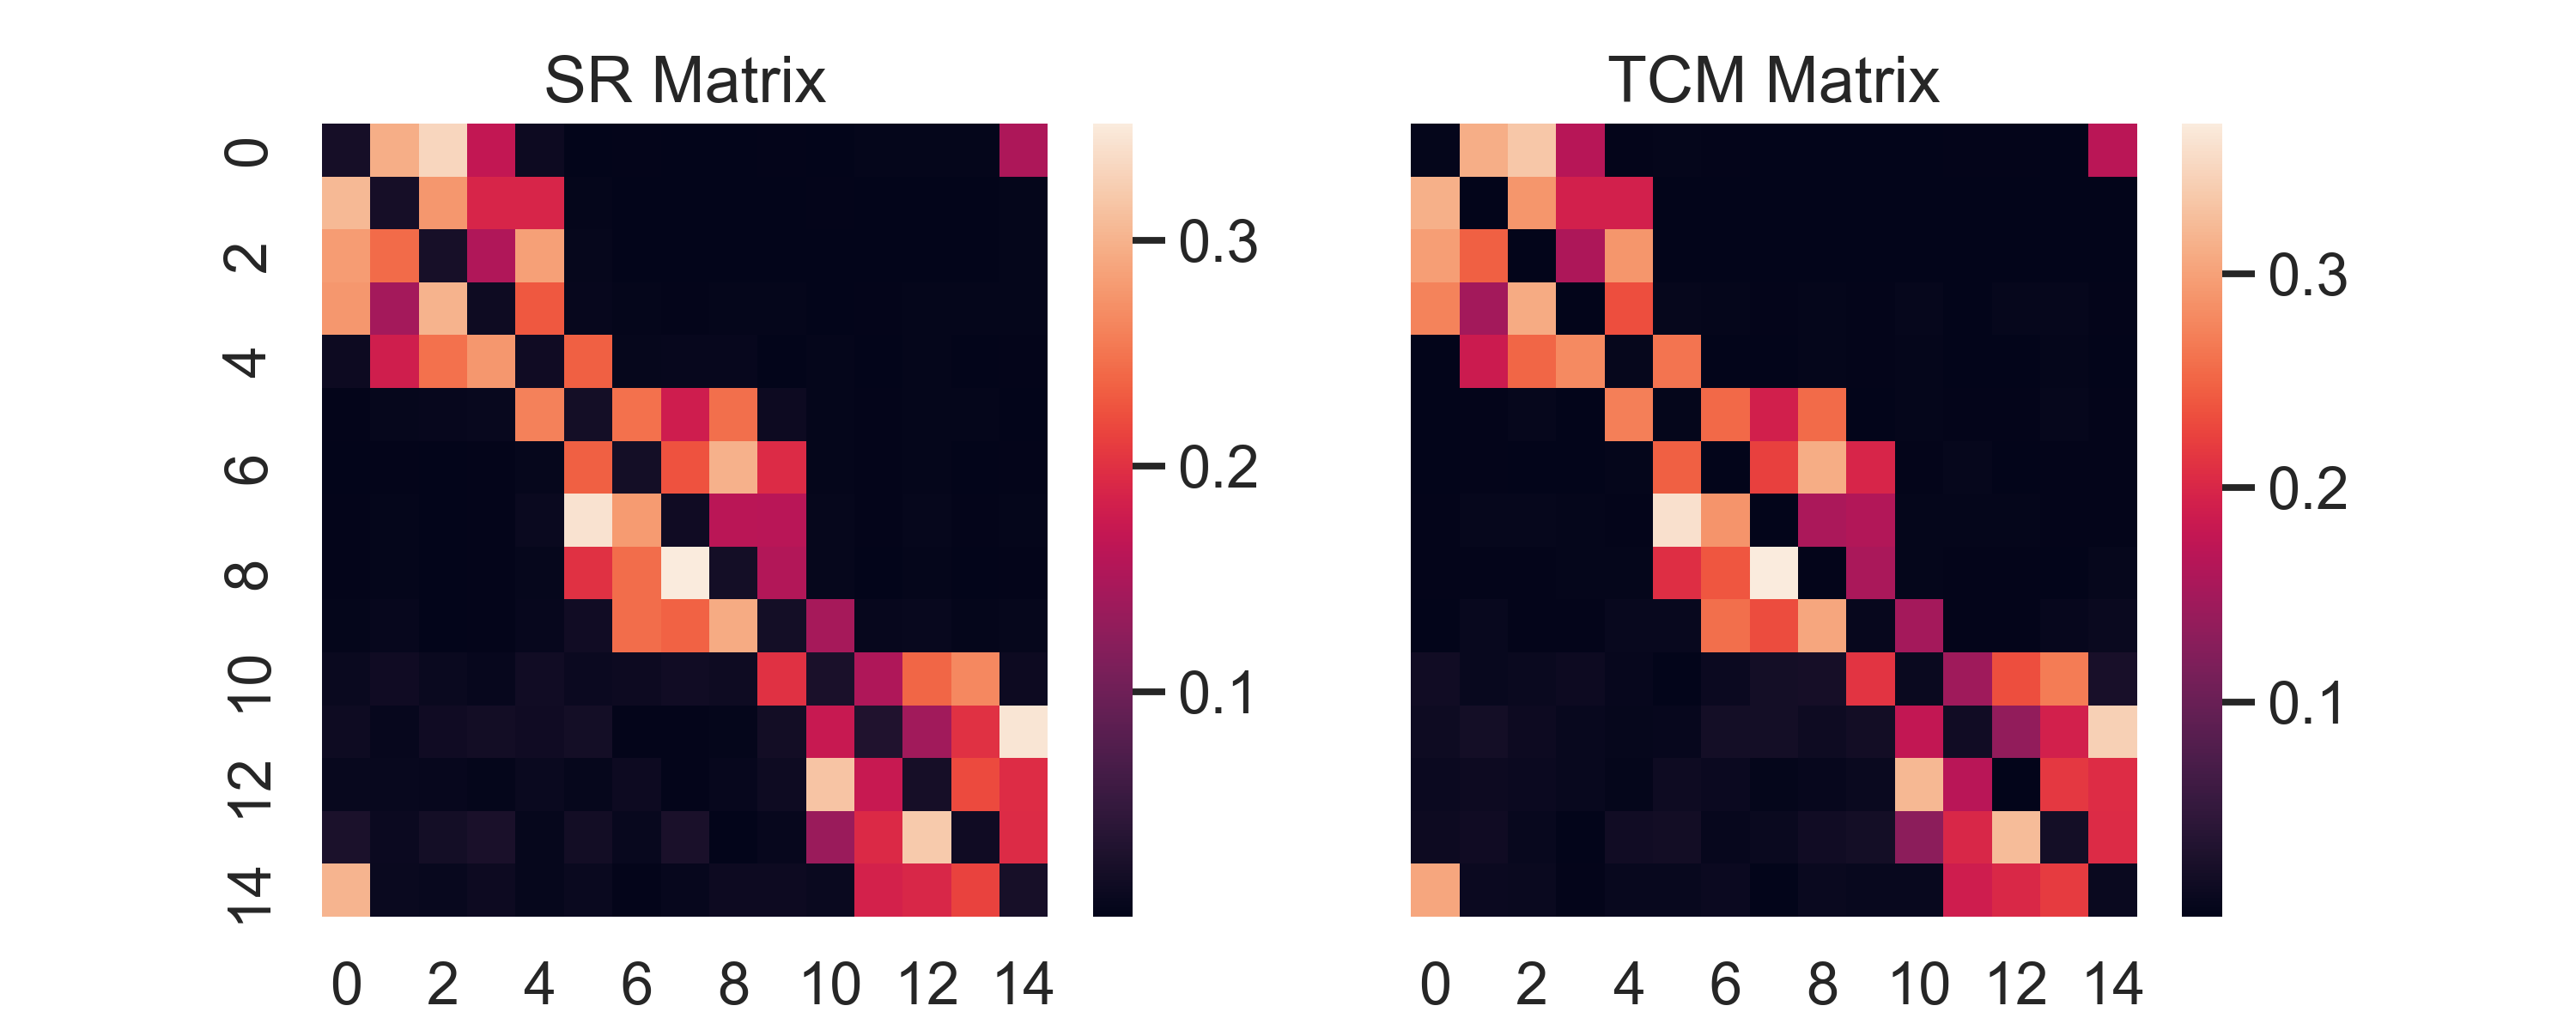
\includegraphics[width = 0.9\textwidth]{chapter_notebooks/chapter_2/figures/SR_vs_TCM_Matrices.png}
	\caption{Successor Representation and Temporal Context Model representations of context following a random walk through the modular graph structure.}
\end{figure}

To model the observed differences in reaction times and link them to the apparent differences shown in Figure \ref{fig:SR-TCM-model-simulations}, we apply principles of information theory. Specifically, we assume that response time for each stimulus is a function of the uncertainty in its surrounding context. Measures of information entropy have previously been used to explain RT differences between cluster transitions while traversing similar graph structures \cite{lynn2020abstract, lynn2020human,lynn2020humans}. Formally, 

\begin{equation}
	\begin{aligned}
		RT(node) \cong Entropy(node) = \sum_{s' \in S} \hat{M}(s, s') * log(\hat{M}(s, s'))
	\end{aligned}
\end{equation}

where $M(s, s')$ is the context representation at node $s$. For SR, this expression evaluates to the expected future visits to state $s'$ from state $s$ whereas for TCM this expression evaluates to the extent to which $s'$ is activated as a result of $s$. 

As noted previously, a common indicator of participants having acquired the global structural knowledge is a slow down in responses when the ongoing stimulus stream crosses a cluster (relative to transitions within a cluster) of the modular graph. Context representations can be used to model the cross cluster transitions by computing a `surprisal' effect. For simulations, the surprisal effect is computed as the Jenson-Shannon distance between the context representations of two nodes. Formally, 

\begin{equation}
	\begin{aligned}
		RT(s \rightarrow s') \cong JS(s, s') = \sqrt[2]{\frac{D(M(s, .) || p) + D(M(s', .) || p)}{2}} \\
	\end{aligned}
\end{equation}

where $M(s, .)$ is the context representation of node vector $s$, $p$ is the point-wise mean of nodes $s$ and $s'$ and $D(M||p)$ is the Kullback-Leibler divergence between probability distributions $M$ and $p$. 

The formalization of observed response time differences due to surprisal (and node entropy) allows us to simulate expected reaction time distributions for novel walk types. Specifically, to understand the mechanisms behind acquiring the global modular graph pattern following a limited exposure, each model was simulated for random walk with lengths of 0, 3, 6, and 999. A random walk length of 0 translates to a completely random selection of one of the 15 nodes of the modular graph on each trial. Walk length of 3 and 6 translate to a random walk visiting 3 and 6 edges (4 and 7 nodes) respectively before being reset to a random node (similar to visiting the Target store in short bursts to purchase relevant items and checking out without visiting the entire store). Finally, a walk length of 999 translates to visiting 999 edges (with repetition) through their connections on the modular graph. Parameters of the simulations in figure \ref{fig:SR-TCM-walklength-matrices} are determined through a best-fitting grid search procedure. Specifically, for a combination of parameters the euclidean distance between the genearted context matrix (SR or TCM) was computed. A grid search was conducted to determine the parameters which minimized this euclidean distance. 

\begin{figure}
	\centering
	\label{fig:SR-TCM-walklength-matrices}
	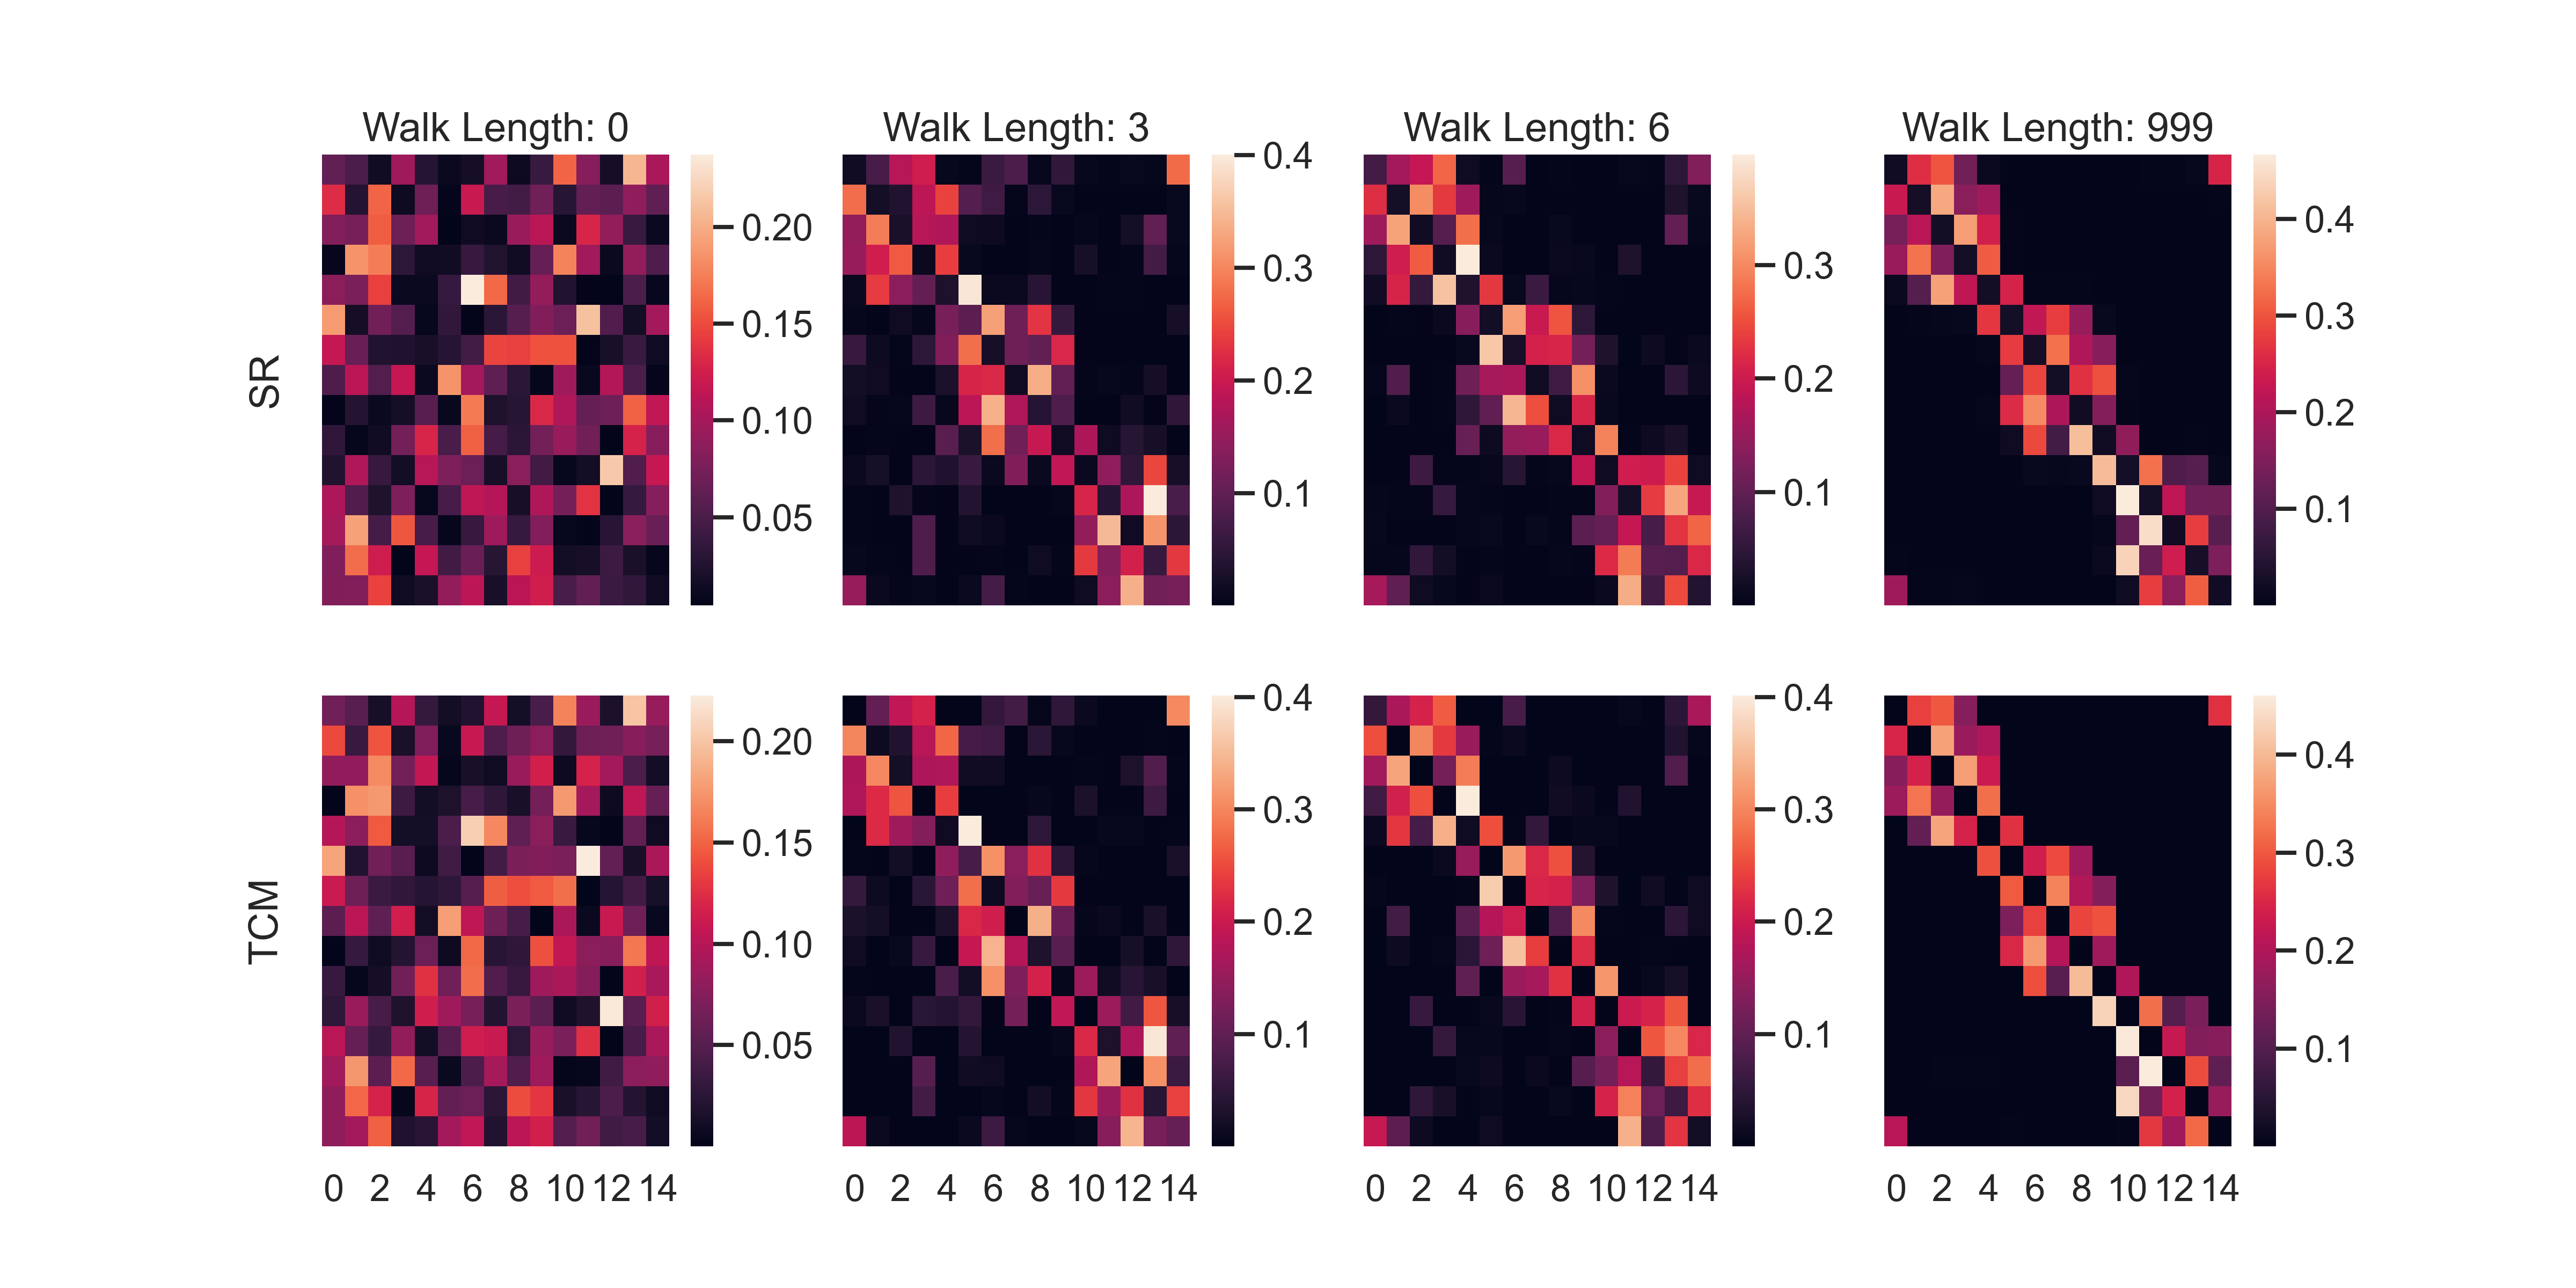
\includegraphics[width = \textwidth]{chapter_notebooks/chapter_2/figures/walk_length_SR_TCM_matrices.png}
	\caption{Model prediction of context representations for SR and TCM models across different walk lengths. Both models seemingly predict that the modular structure of the original graph is increasingly recovered with longer walk lengths.}
\end{figure}

The acquisition of the global structure can be modeled using surprisal as has been done in previous research \cite{lynn2020abstract,lynn2020humans,lynn2020human}. For a subset of parameters in the valid range of 0 to 1, each model was simulated to produce a context matrix. Jensen-Shannon distance was computed between each pairs of nodes and averaged over cross-cluster pair and within cluster pairs. Simulation results below show the transition Jensen-Shannon distances over 100 simulations of the model for each parameter combination. For SR, `param\_a' is the learning rate parameter $\alpha$ and `param\_b' is the discount parameter $\gamma$. For TCM, `param\_a' is the learning rate parameter $\alpha$ and `param\_b' is the context drift parameter $\rho$. 
\begin{figure}
	\centering
	\label{fig:SR-TCM-walklength-transition-sjdist}
	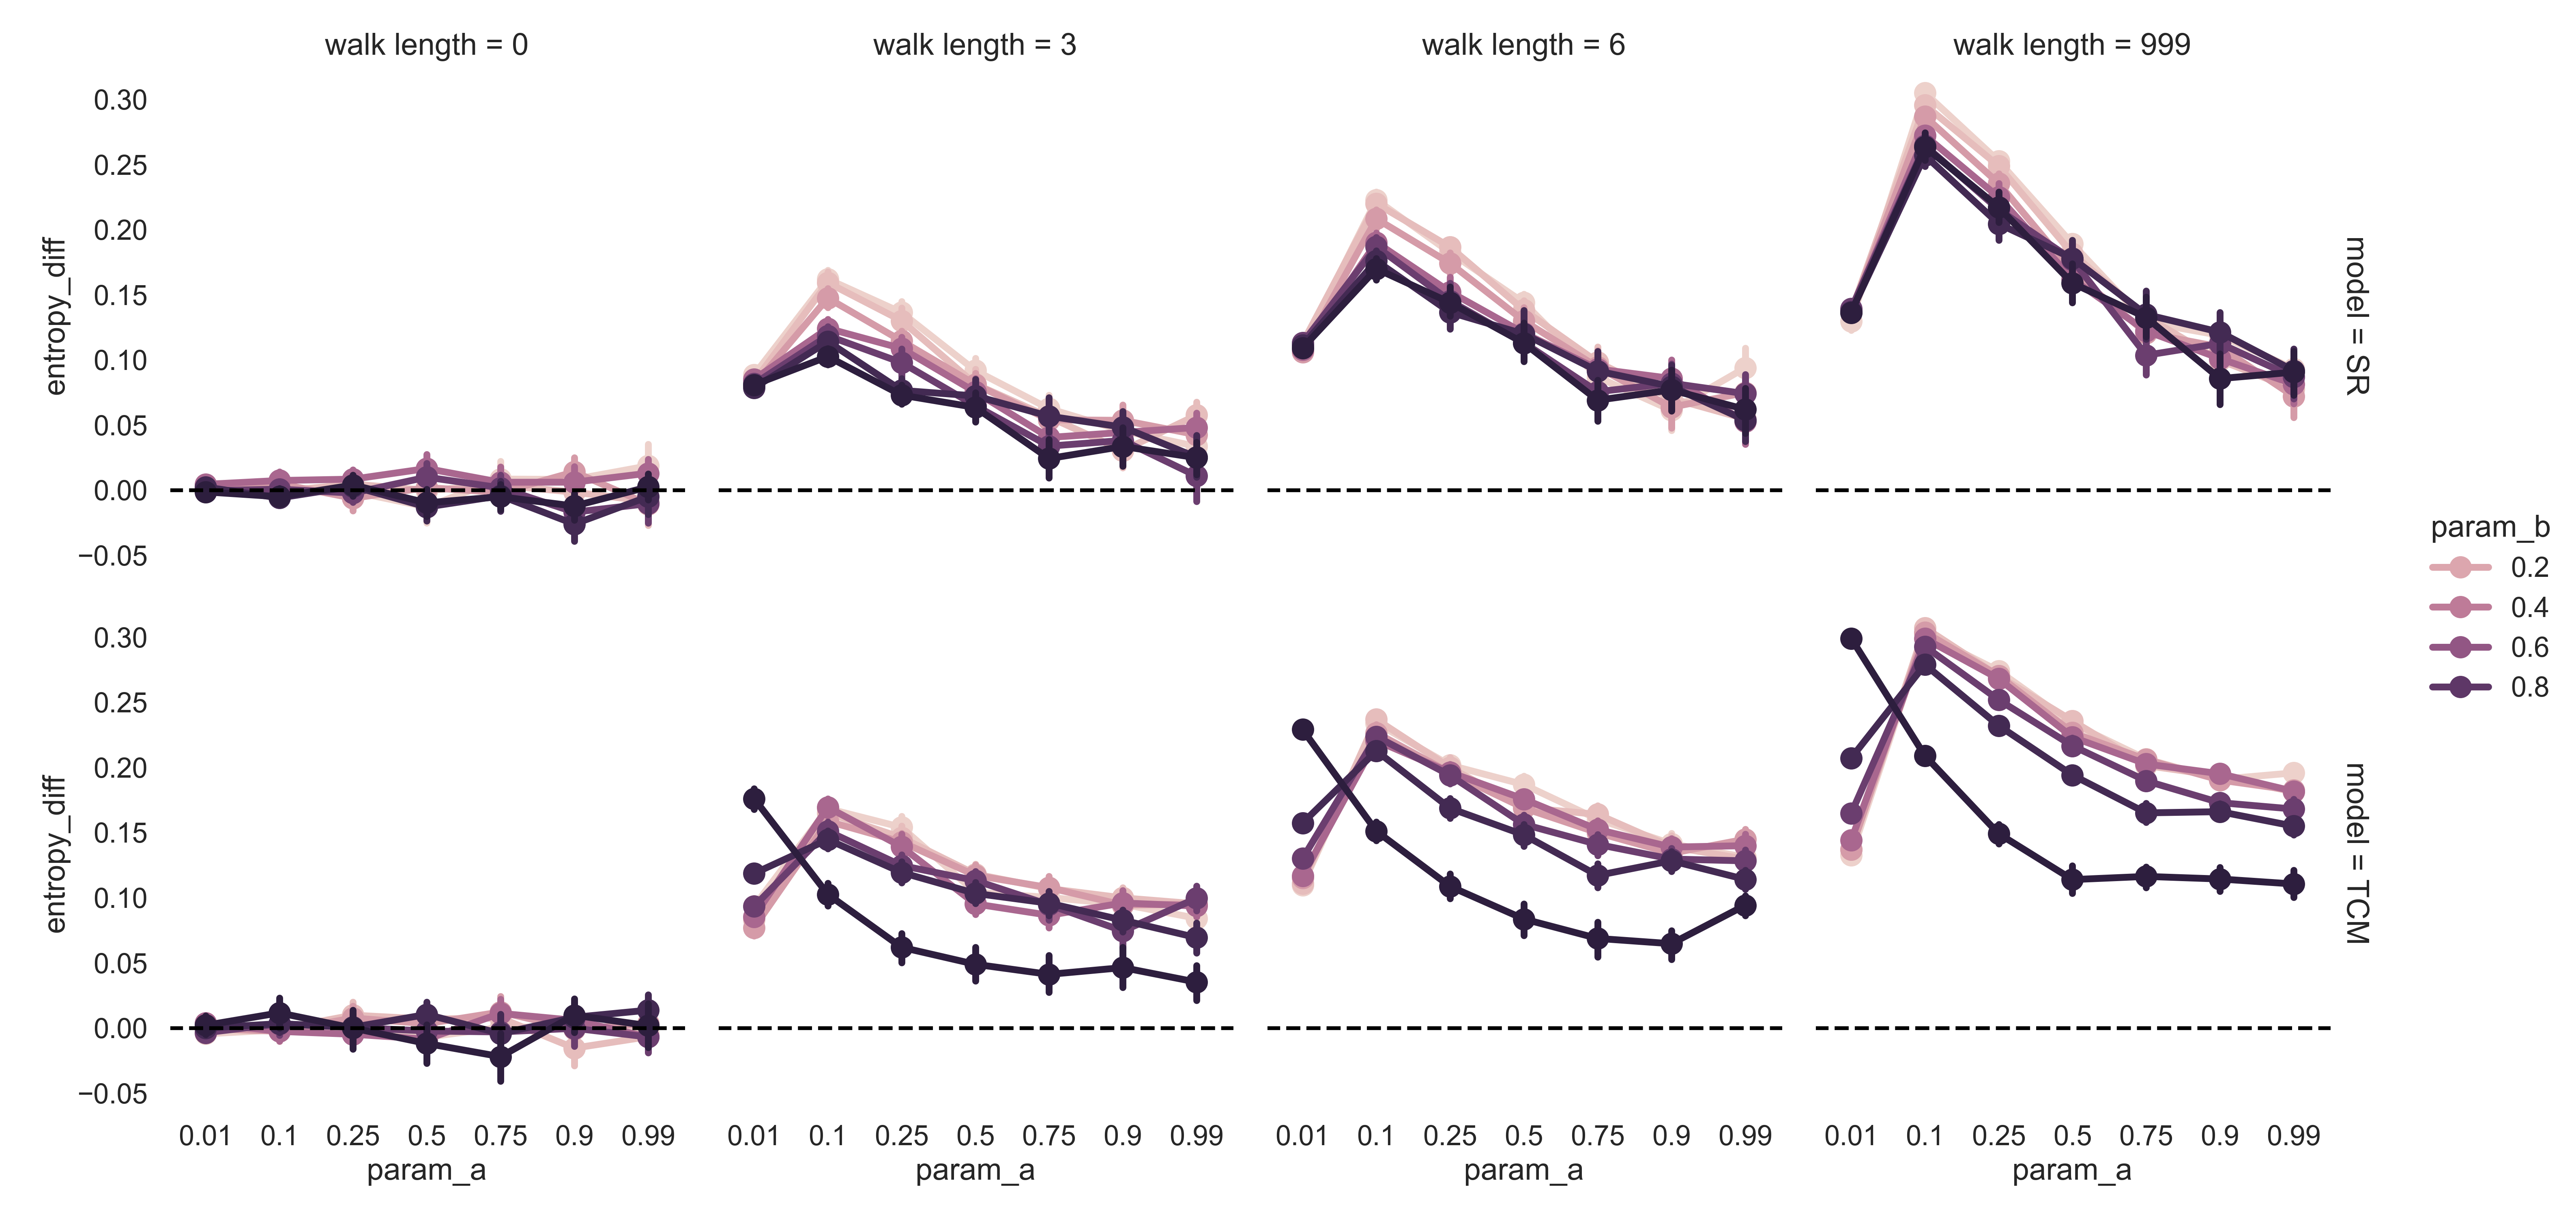
\includegraphics[width = \textwidth]{chapter_notebooks/chapter_2/figures/SR_TCM_boundary_nonboundary_jsdist.png}
	\caption{Model Predictions for differences in reaction time comparing across cluster transitions to within cluster transitions across walk lengths. Both models predict that cross cluster surprisal effect will increase with walk length leading to an increased reaction time.}
\end{figure}

Figure \ref{fig:SR-TCM-walklength-transition-sjdist} shows that both context models predict an increased surprisal as walk length through the modular graph gets longer. As walk length increases, context associated with each node increasingly represents neighboring nodes. Since neighbors of the boundary nodes differ more than those between the non-boundary nodes, crossing from a boundary node to another boundary nodes.

The two context models, however, differ in their predictions in the role of a boundary node. Figure \ref{fig:SR-TCM-walklength-boundary-nonboundary-entropydiff} shows that SR predicts an increased entropy in its representation of the boundary nodes with walk length relative to the non-boundary nodes for some values of the $\alpha$ and $\gamma$ parameters. On the other hand the TCM does not predict such increased in Boundary vs Non Boundary entropy differences. 
\begin{figure}[ht]
	\centering
	\label{fig:SR-TCM-walklength-boundary-nonboundary-entropydiff}
	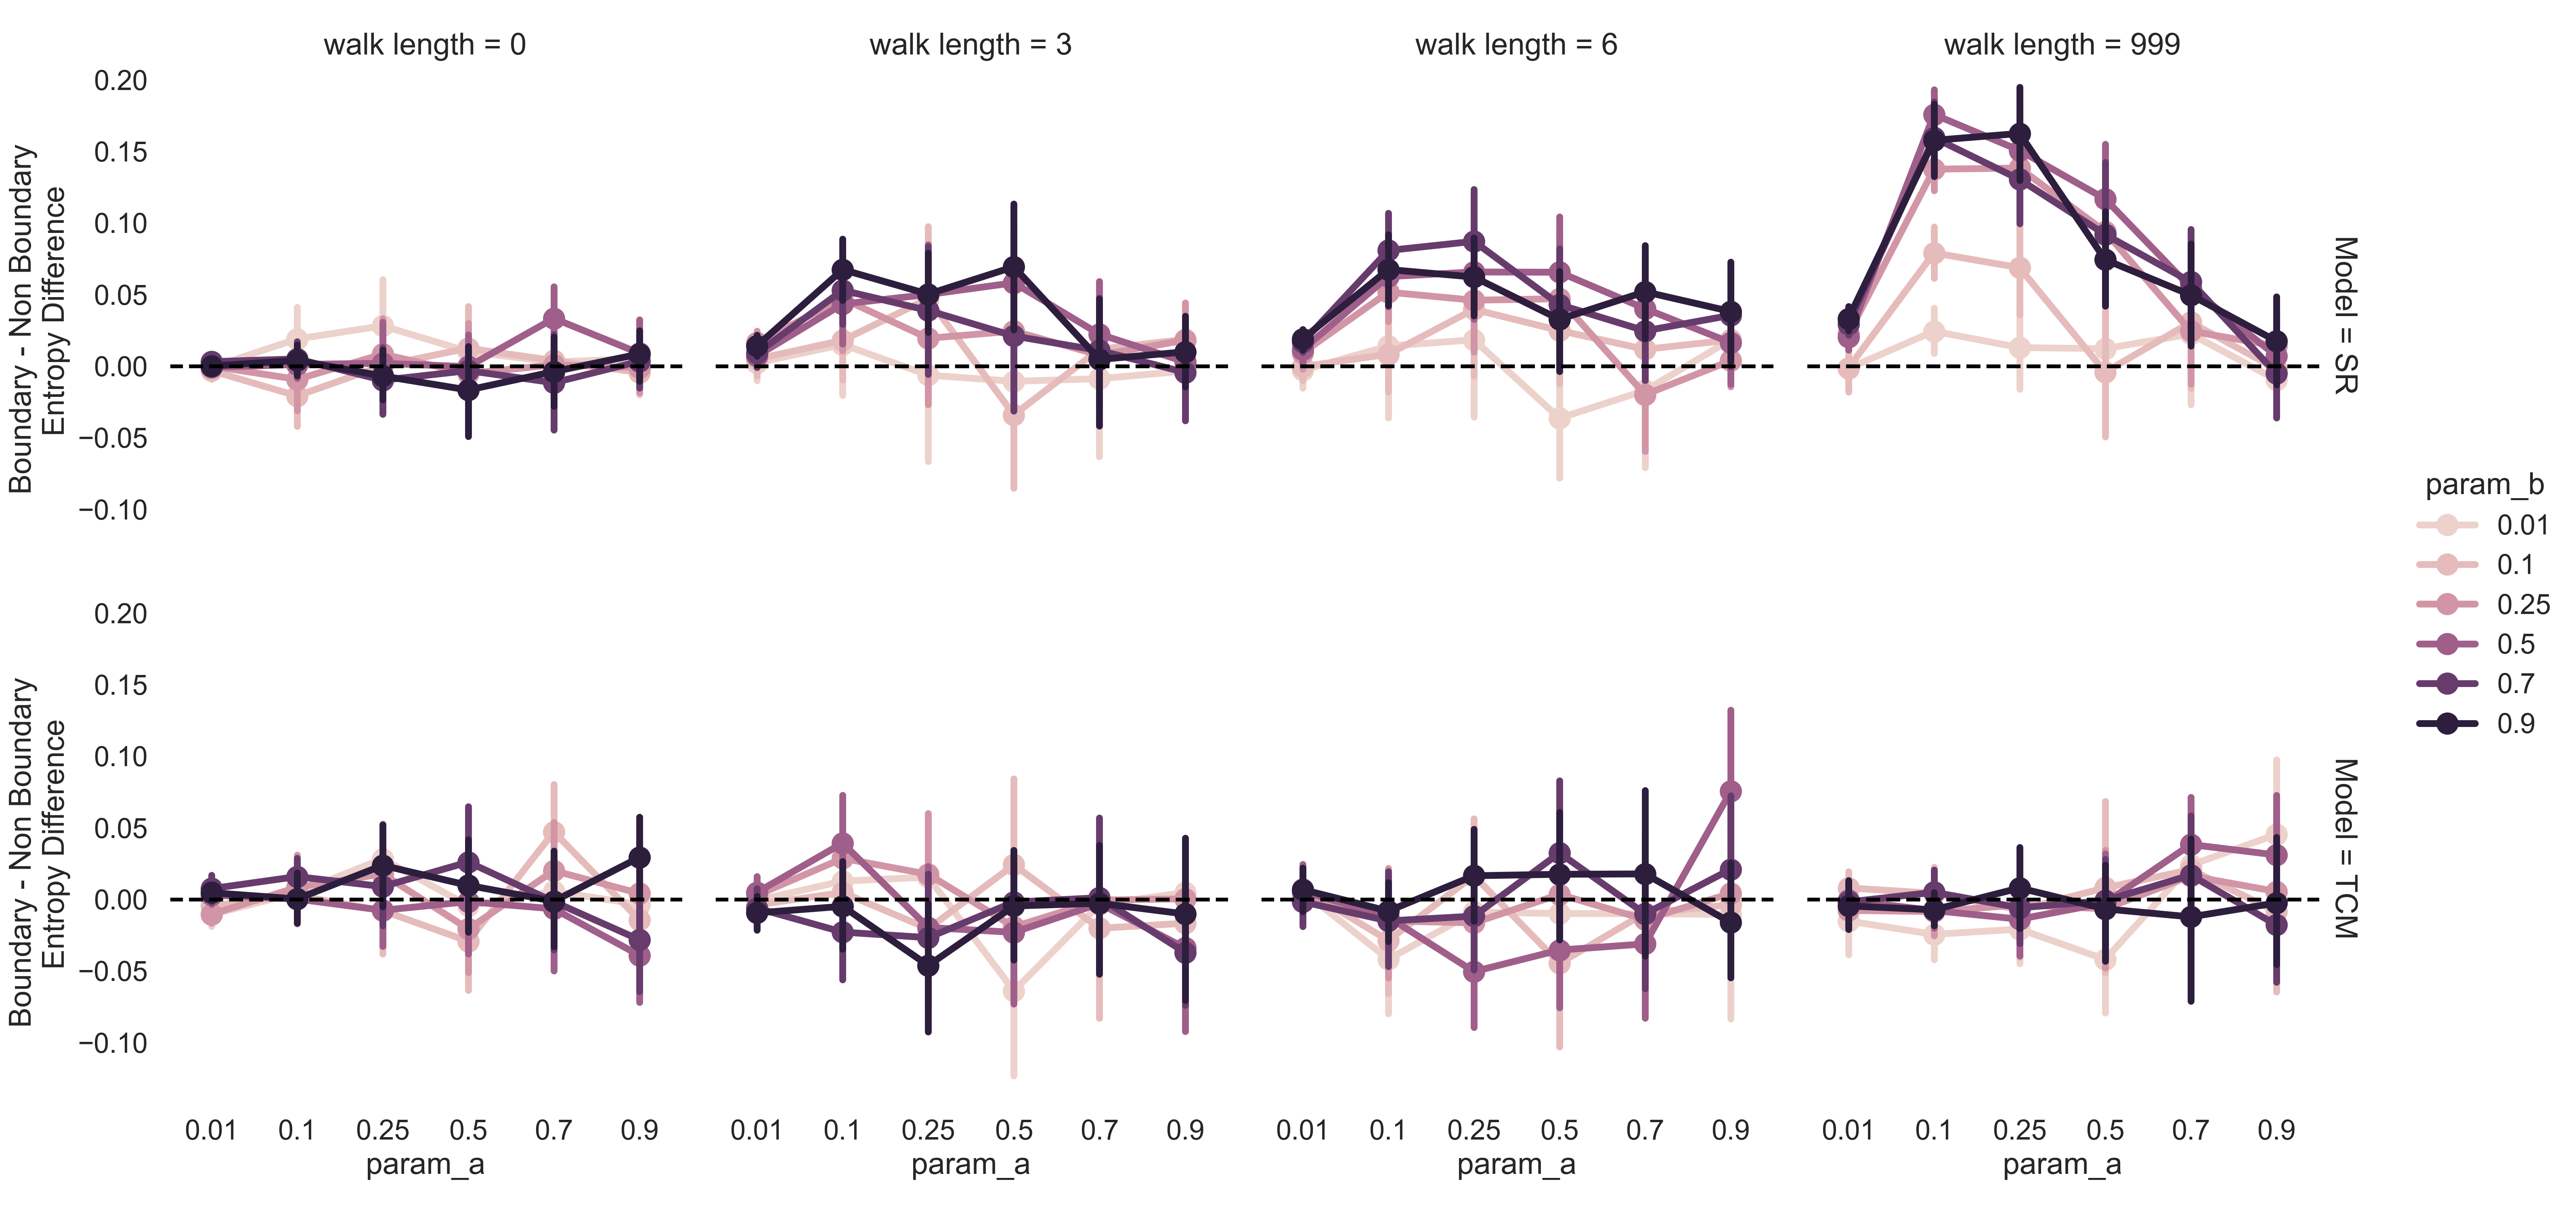
\includegraphics[width = \textwidth]{chapter_notebooks/chapter_2/figures/SR_TCM_walklength_boundary_nonboundary_entropydiff.png}
	\caption{Model prediction differences between the SR and the TCM after different walk lengths. SR predicts that entropy of boundary nodes will scale with walk lengths whereas TCM does not.}
\end{figure}


The predictive nature of SR (as modeled by the future discount, $\gamma$ parameter) allows for a representation of nodes in the neighboring cluster to impact entropy on the boundary node of the current cluster that leads to that neighboring cluster. This effect is unique on boundary nodes of a cluster as non-boundary nodes of the second cluster are closer to the immediate neighbor of the current cluster (i.e. the boundary node that serves as an entry point to the second cluster) Since TCM is associative (as opposed to predictive), each node activates its immediate and two-step neighbors with equal weight. associative nature of TCM does not transfer representations of nodes of the neighboring cluster to the boundary node of the current cluster. Rescaled heatmap in figure \ref{fig:zoomed-in-SRTCM-boundary-entropy} presents this effect.

\begin{figure}[ht]
	\centering
	\label{fig:zoomed-in-SRTCM-boundary-entropy}
	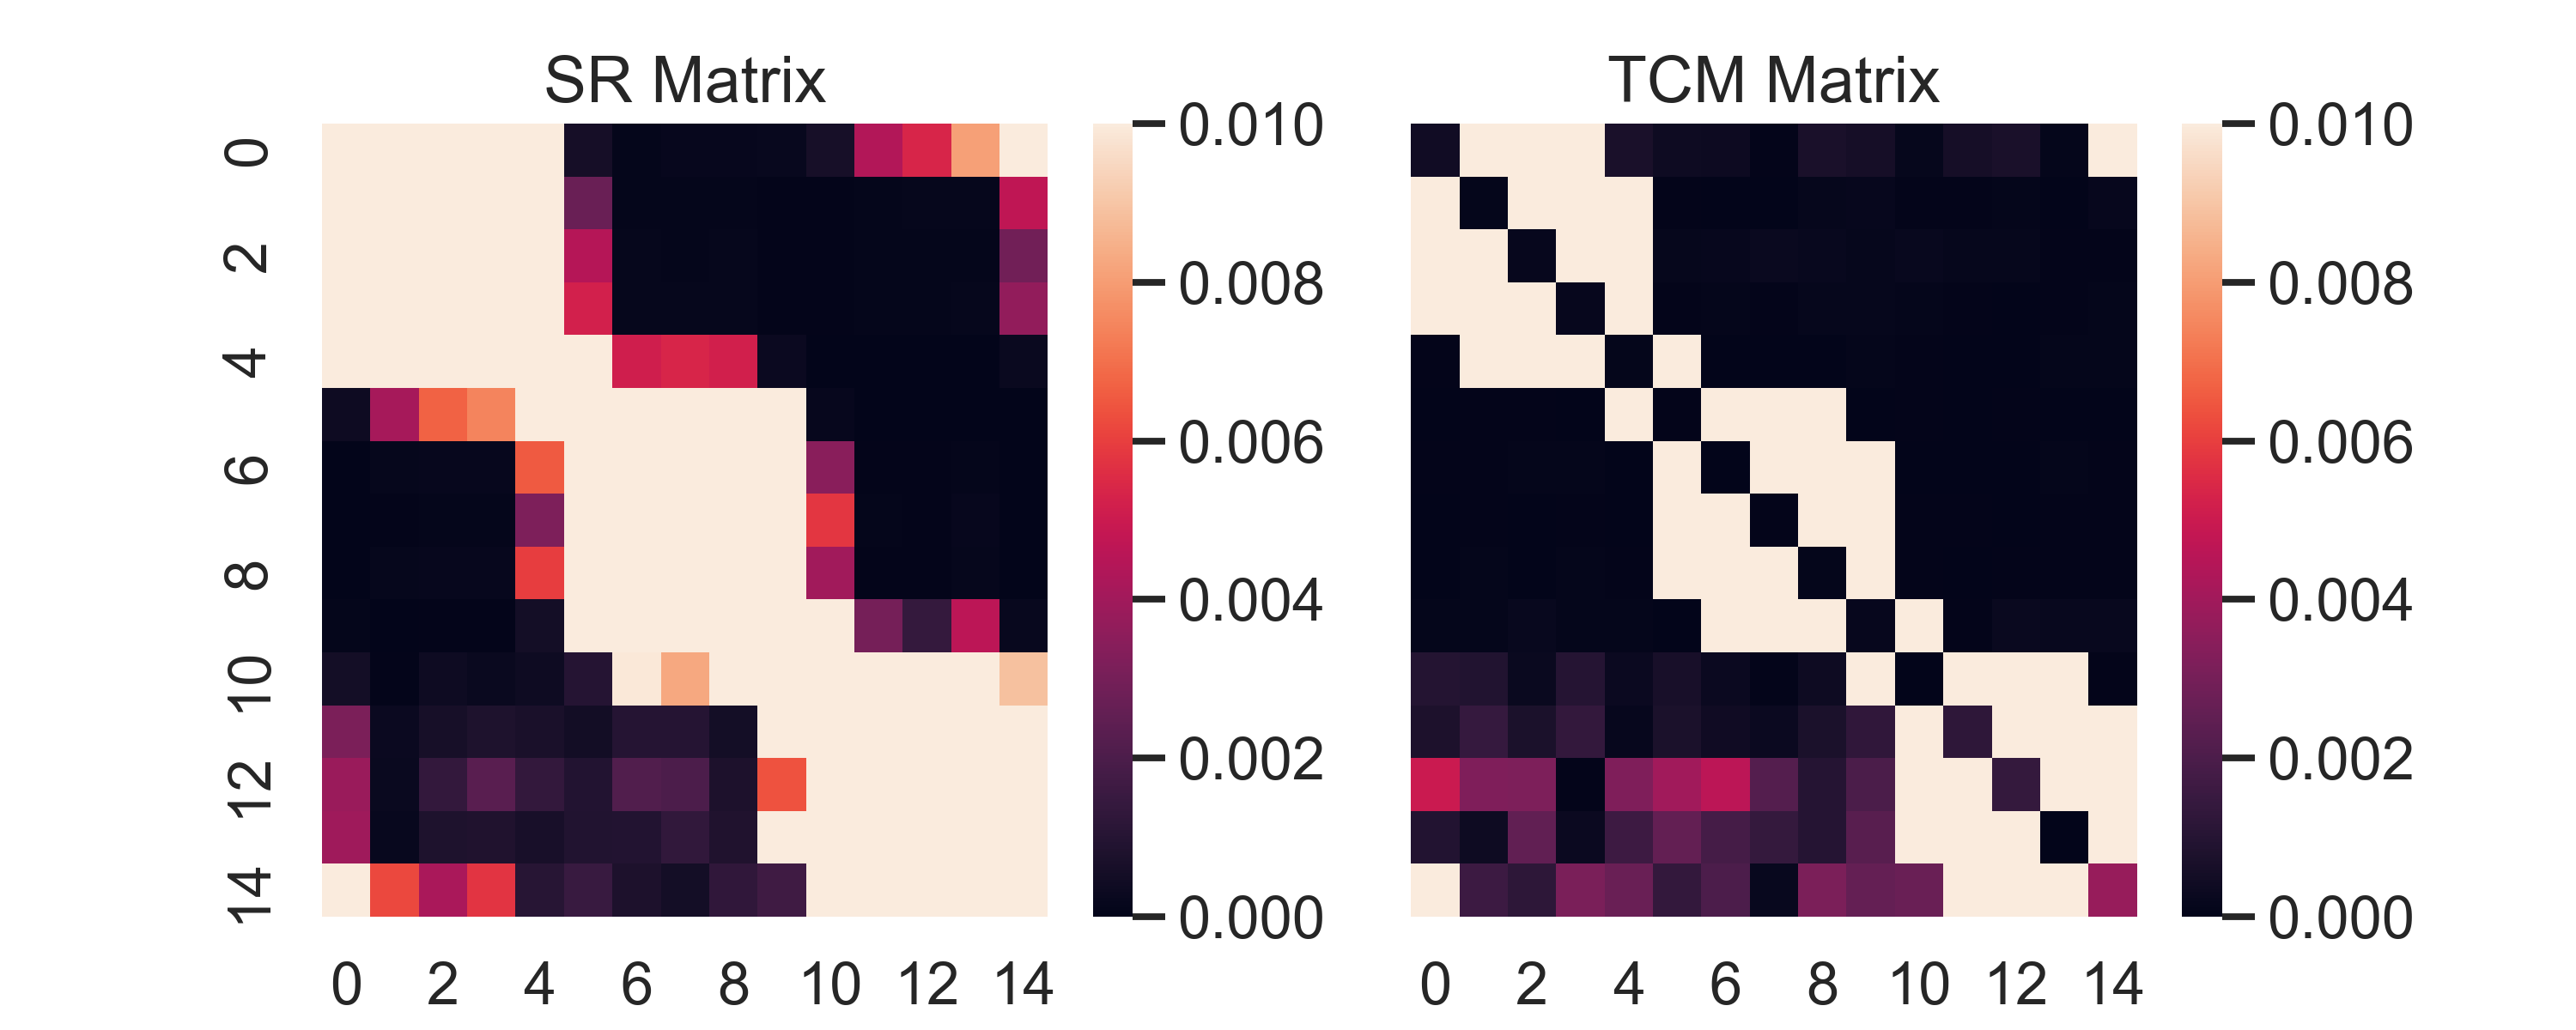
\includegraphics[width = \textwidth]{chapter_notebooks/chapter_2/figures/SR_vs_TCM_Matrices_zoomed.png}
	\caption{Rescaled SR and TCM matrices depict differences between context representations of the two models. Boundaries in SR incorporate more information than those in TCM.}
\end{figure}

The SR-based predictive context representation in particular shows that boundary nodes carry more information than non-boundary nodes whereas the associative context representation does not produce this effect. \footnote{The activity in the lower third of both matrices is due to recency; while these are interesting patterns, and seem to indicate that SR can account for the recency effects in memory which was the primary motivation behind introduction of the TCM \cite{gershman2012successor,howard2005temporal}. Investigating recency effects in this implicit statistical learning context is out of scope for this dissertation.}

Thus, both SR and TCM models would predict slow down in cross-cluster transitions relative to within cluster transitions, and that this slow down will increase with walk length. However predictive context representations through SR is unique in predicting the scaled slow down at boundary nodes with random walk length, \textit{independent} of transitions. While lack of a scaled slow down to boundary nodes does not invalidate the SR model (because some values of the parameters allows SR to not scale the slowed reactions with walk length), the presence of such a slow down provides evidence for predictive representations in such statistical learning tasks. The study presented next, thus tests this prediction. 

%The SR model, while underlies the reinforcement learning principle does not rely on the availability of explicit rewards at the end to build a predictive representation for each step. For this dissertation, I will similarly assume that predictive representations are learned from experience through the environment without the need for an explicit goal state.





\newpage
\chapter{Comparing Implicit Event Boundaries with Explicit Event Boundaries}
\label{chapter-3-implicit-explicit-event-boundaries}
\section{Introduction}
We receive a continuous stream of sensory information in our daily lives. In order to make sense of it, we often parse it into meaningful chunks for storage, retrieval and comprehension. For example, we may recall our drive to work as a series of discrete events; got into the car, got coffee, picked up a collegue, hit traffic on a particular street, parked, and walked over to the office. What aspects of the incoming stream help us organize continuous temporal information in such discrete chunks? 
Temporal chunking in cognitive psychology has been studied under several domains from event boundaries \cite{clewett2019transcending, zacks2007event, rouhani2020reward,rouhani2018dissociable,dubrow2013influence,baldwin2008segmenting}, language learning, \cite{romberg2010statistical,knowlton1992intact}, categorization \cite{unger2022ready,gabay2015incidental}, and motor sequencing \cite{bera2021motor, tremblay2010movement, savalia2016unified,ostlund2009evidence}. Chunking a repeated sequence of experiences is crucial to abstracting patterns in the environment and formation of habits for quick and efficient interactions with the environment \cite{dezfouli2012habits, smith2016habit,dolan2013goals, dezfouli2014habits, gershman2010learning, botvinick2012hierarchical}. 

Models of temporal event segmentation suggest that the points which lead to temporal segmentation seem to be unique in their properties in both segmenting the continuous stream of information and integration of information across the temporal event. These `event boundaries' are, for example, shown to be remembered better \cite{swallow2009event,rouhani2018dissociable,rouhani2018dissociable, zacks2020event, radvansky2017event, heusser2018perceptual}, serve as points of retrieval \cite{michelmann2023evidence} and replay to promote long term memory \cite{hahamy2023human, sols2017event} and easy parsing, help integrate memory across time \cite{clewett2019transcending}, and separates across boundary events while collapsing within boundary events \cite{clewett2019transcending, lositsky2016neural,ezzyat2014similarity, brunec2018boundaries}. 

In most prior studies, event boundaries have been studied using explicit context shifts. For example, when stream of stimuli are surrounded by colored border, event boundaries are operationalized by first showing the stimuli surrounded by a color and abruptly changing that color\cite{heusser2018perceptual}. In another study, event boundaries were operationalized via explicit context changes by changing the associated stimulus\cite{ezzyat2014similarity}. A pair of images were presented on each trial; one image of the pair, the 'scene' image remained constant for a short sequence of trials whereas the other ('object' or 'face') changed on each trial. Participants were asked to make judgments about the object/face image \cite{ezzyat2014similarity}. Previously, context changes had been operationalized as either perceptual or semantic shift in ongoing set of events by having participants watch clips \cite{swallow2009event}. In more recent work, context change has been operationalized as changes in ongoing reward contingencies associated with each stimulus \cite{rouhani2020reward}. 

Consistent findings across most studies in explicitly operationalized event boundaries show that event boundaries are often remembered better \cite{swallow2009event, radvansky2017event, heusser2018perceptual,clewett2019transcending, rouhani2020reward,ezzyat2014similarity,baldassano2017discovering}, and events across boundaries appear to be perceptually farther whereas events within boundaries appear to be perceptually closer \cite{clewett2019transcending,ezzyat2014similarity,brunec2018boundaries,lositsky2016neural}. In recent work, however, it has been shown that event boundaries can also be formed \textit{without} explicit changes in context. After being exposed to a stream of stimuli such that the ordering is controlled by a modular graph shown in figure \ref{fig:modular_graph}, participants seem to recognize across cluster transitions as `natural breaks' more often than within cluster transitions \cite{schapiro2013neural}. In recent work, this finding has been linked to statistical learning of temporal graph structures \cite{karuza2022value,karuza2019human,kahn2018network,kahn2018network,lynn2020abstract,lynn2020human,lynn2020humans} and measured by slowed reaction times across clusters than within clusters. However, past studies where boundaries are operationalized implicitly do not assess the memory representations of these boundaries using the same tests used in explicitly operationalized boundary paradigms. 

In this chapter, I present two tests on implicitly operationalized boundaries to assess whether they elicit the same behavioral properties as the explicitly operationalized boundaries. In particular, I use the paradigm and graph structure previously used in Schapiro et al. \cite{schapiro2013neural} to test whether participants recall boundary items better (or worse) than non-boundary items. I then use a two module graph structure in Figure \ref{fig:two_module_graph} to test whether items across the two clusters appear farther than items within a cluster (similar to findings in explicitly operationalized boundary paradigms). 

\section{Modeling Boundary Memory Benefits}
Event segmentation theory suggests that the segmentation of the continuous sensory experience occurs automatically and through prediction errors\cite{zacks2007event,zacks2007eventp, swallow2009event}. According to the event segmentation theory, we maintain an ongoing `context' which is predictive of upcoming events. Event boundaries are created when this prediction breaks. More recent work has shown that prediction errors are not necessary for creation of event boundaries; a change in uncertainty of the upcoming events can also produce event boundaries \cite{shin2021structuring}. Prediction errors particularly lose their value in learning new information when the explored environment is uncertain\cite{behrens2007learning}. Nevertheless, under environments with high regularities, prediction errors remain the key mechanisms driving boundary formation. 

As reviewed above, prediction errors need not be explicitly operationalized for an event boundary to be learned. Prediction errors which imply shifts in ongoing context, similar to implicitly operationalized event boundaries may be implicit. In chapter \ref{chapter-2-walk-lengths-modulate-statistical-learning} show that context models can be used to estimate representations of implicitly operationalized event boundaries. Particularly, predictive representations such as the SR provide a natural representation of event boundaries which form bottlenecks in transitioning between clusters in modular graphs in figure \ref{fig:modular_graph}. I propose that the same predictive context-representation framework using the Successor Representation model of Reinforcement Learning \cite{dayan1993improving, momennejad2017successor, russek2017predictive, momennejad2020learning,gershman2012successor} can be used to model differences in memory representations. 

To simulate a recognition memory task, I employ a simplified version of the exemplar-based Generalized Context Model \cite{nosofsky2011generalized,nosofsky1986attention, nosofsky2011short}. The GCM follows a class of global matching exemplar models where each studied item is stored as an image or an exemplar in memory. At test, the presented test item is matched with memory representations of stored exemplars by computing the psychological similarity between them. It is assumed that if the similarity, summed over all similarities of the test items with exemplars in memory, crosses a criterion (a free parameter), the participant recognizes that item and the `old' response is chosen in the old/new recognition test. Similarly, a `new' response is chosen when the summed similarity of the test item with all stored exemplars falls below the decision criterion. 

The GCM model for recognition memory can be formalized with the following equations \cite{nosofsky2011short}:

\begin{equation}
    \begin{aligned}
        d_{ij} = [\sum\limits_{k = 1}^K w_k(x_{ik} - x_{jk})^2]^{1/2} \\
        s_{ij} = \exp^{-c_jd_{ij}} \\
        a_{ij} = m_js_{ij}
    \end{aligned}
\end{equation}    

where $d_{ij}$ is the psychological distance between test item $i$ and examplar $j$, $w_k$ is the weight a participant may place on the $k^{th}$ dimensions (and $k \in K$). The distance metric is thus computed as an euclidean distance between exemplars in memory and the test item weighted by where each feature is allowed to have a different weight to reflect differentially important features. $s{ij}$ is the similarity between test item $i$ and exemplar $j$ which decreases exponentially with psychological distance. $c_j$ is a scaling factor determining how much the similarity falls off for a unit of distance for each exemplar. $a_{ij}$ is the activation of exemplar $j$ when compared with test item $i$ and is scaled by the memory strength of the exemplar $m_j$. 

To demonstrate the potential role of temporal structure, a few simplifying assumptions are  made to the recognition memory model. Specifically, in simulations presented below, it is assumed that the each feature dimension of the studied (and test) items is weighted equally. Furthermore, the scaling parameter $c$ is assumed to be 1 for all exemplars. To simulate the differences between boundary and non-boundary nodes in memory, it is assumed that the memory strength of an item associated with each node is proportional to the entropy in its successor representation of that node. While evidence for relating memory strength to context based entropy is scarce, past work has shown that entropy (as a measure of uncertainty) has been a helpful factor in motivated learning and is a contributing factor in hippocampal activation \cite{davis2012striatal}. Furthermore, the slow down associated with increased entropy as demonstrated in previous statistical learning tasks \cite{lynn2020abstract,lynn2020human,lynn2020humans} implies that participants at the least spend more time on such high-entropy boundary nodes, thereby allowing for a better chance of remembering these nodes better. 

Given these assumptions, simulating recognition memory on the final SR representation provides an expected comparison of recognition memory acccuracy for old boundary, old non-boundary and new items. Figure \ref{fig:recog_memory_sims_with_criterion} shows the what this modeling approach expects. On average, implicitly operationalized boundaries are expected to be remembered better than non-boundaries. This benefit is expected to be apparent for participants who are exposed to the temporal structure (right panel) relative to participants who are not (left panel).

\begin{figure}[ht]
    \label{fig:recog_memory_sims_with_criterion}
    \centering
    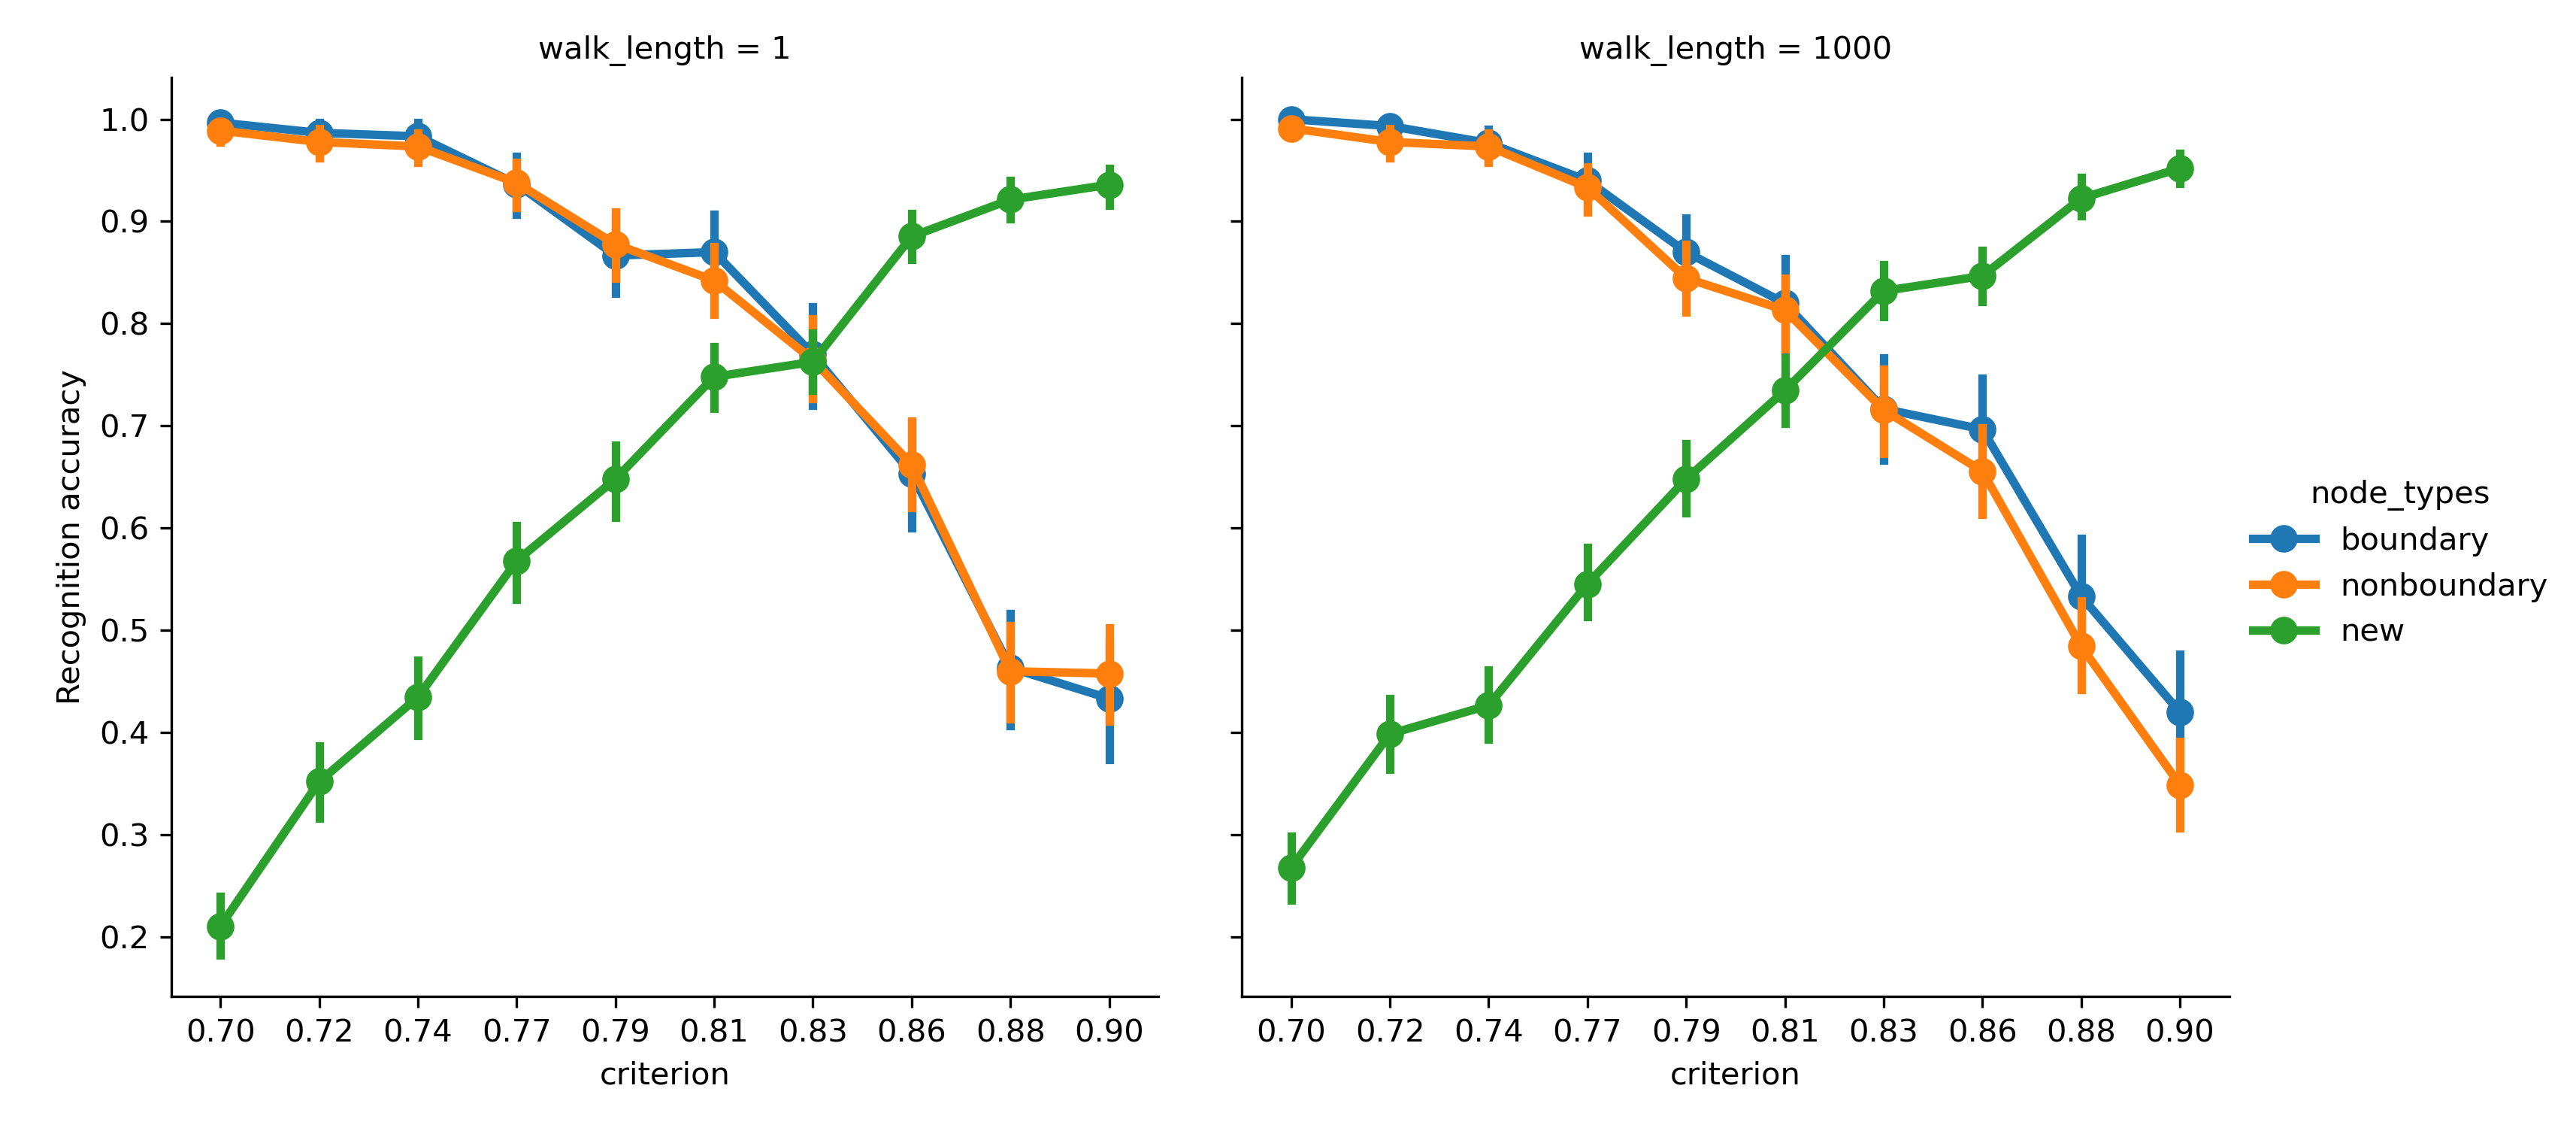
\includegraphics[width = \textwidth]{chapter_notebooks/chapter_3/figures/recog_memory_with_criterion.png}
    \caption{Simulated recognition memory test performances for walk lengths of 1 and walk lengths of 1000 on modular graph in Figure \ref{fig:modular_graph}. On average, recognition memory performance is expected to be better for boundary items than non-boundary items.}
\end{figure}



\section{Methods}
\subsubsection*{Participants}
57 undergraduate students at the University of Massachusetts Amherst participated in this study. Participants were at least 18 years of age and were compensated via course credit. All procedures were approved by the University Institutional Review Board. 

\subsubsection*{Design and Procedures}
Participants were randomly assigned to either a structured exposure or an unstructured exposure group. The overall experimental procedures were the same across both groups. 

Randomly generated polygon shapes were used as stimuli for this experiment. At the beginning of the study, participants were shown 15 polygons which formed the primary stimuli for this study. Participants were asked to carefully study these polygons and to remember their orientation. During 750 exposure trials, separated into 3 blocks of 250, participants were presented these polygons one at a time and asked to judge whether the presented polygon was in its canonical orientation or rotated. Polygons were further surrounded by a (purple, orange, or dark green) colored border.

Each polygon with its border was associated with a node in the three-module graph in figure \ref{fig:modular_graph}. Order of polygons during exposure was determined by a participant's group. The order for 27 participants in the structured exposure group was determined by a random walk through the 3-module graph whereas that for 30 participants in the unstructured group was determined by a random selection among the 15 items (similar to a random walk of length 0). 

\begin{figure}[ht]
    \centering
    \label{fig:exp2-design}
    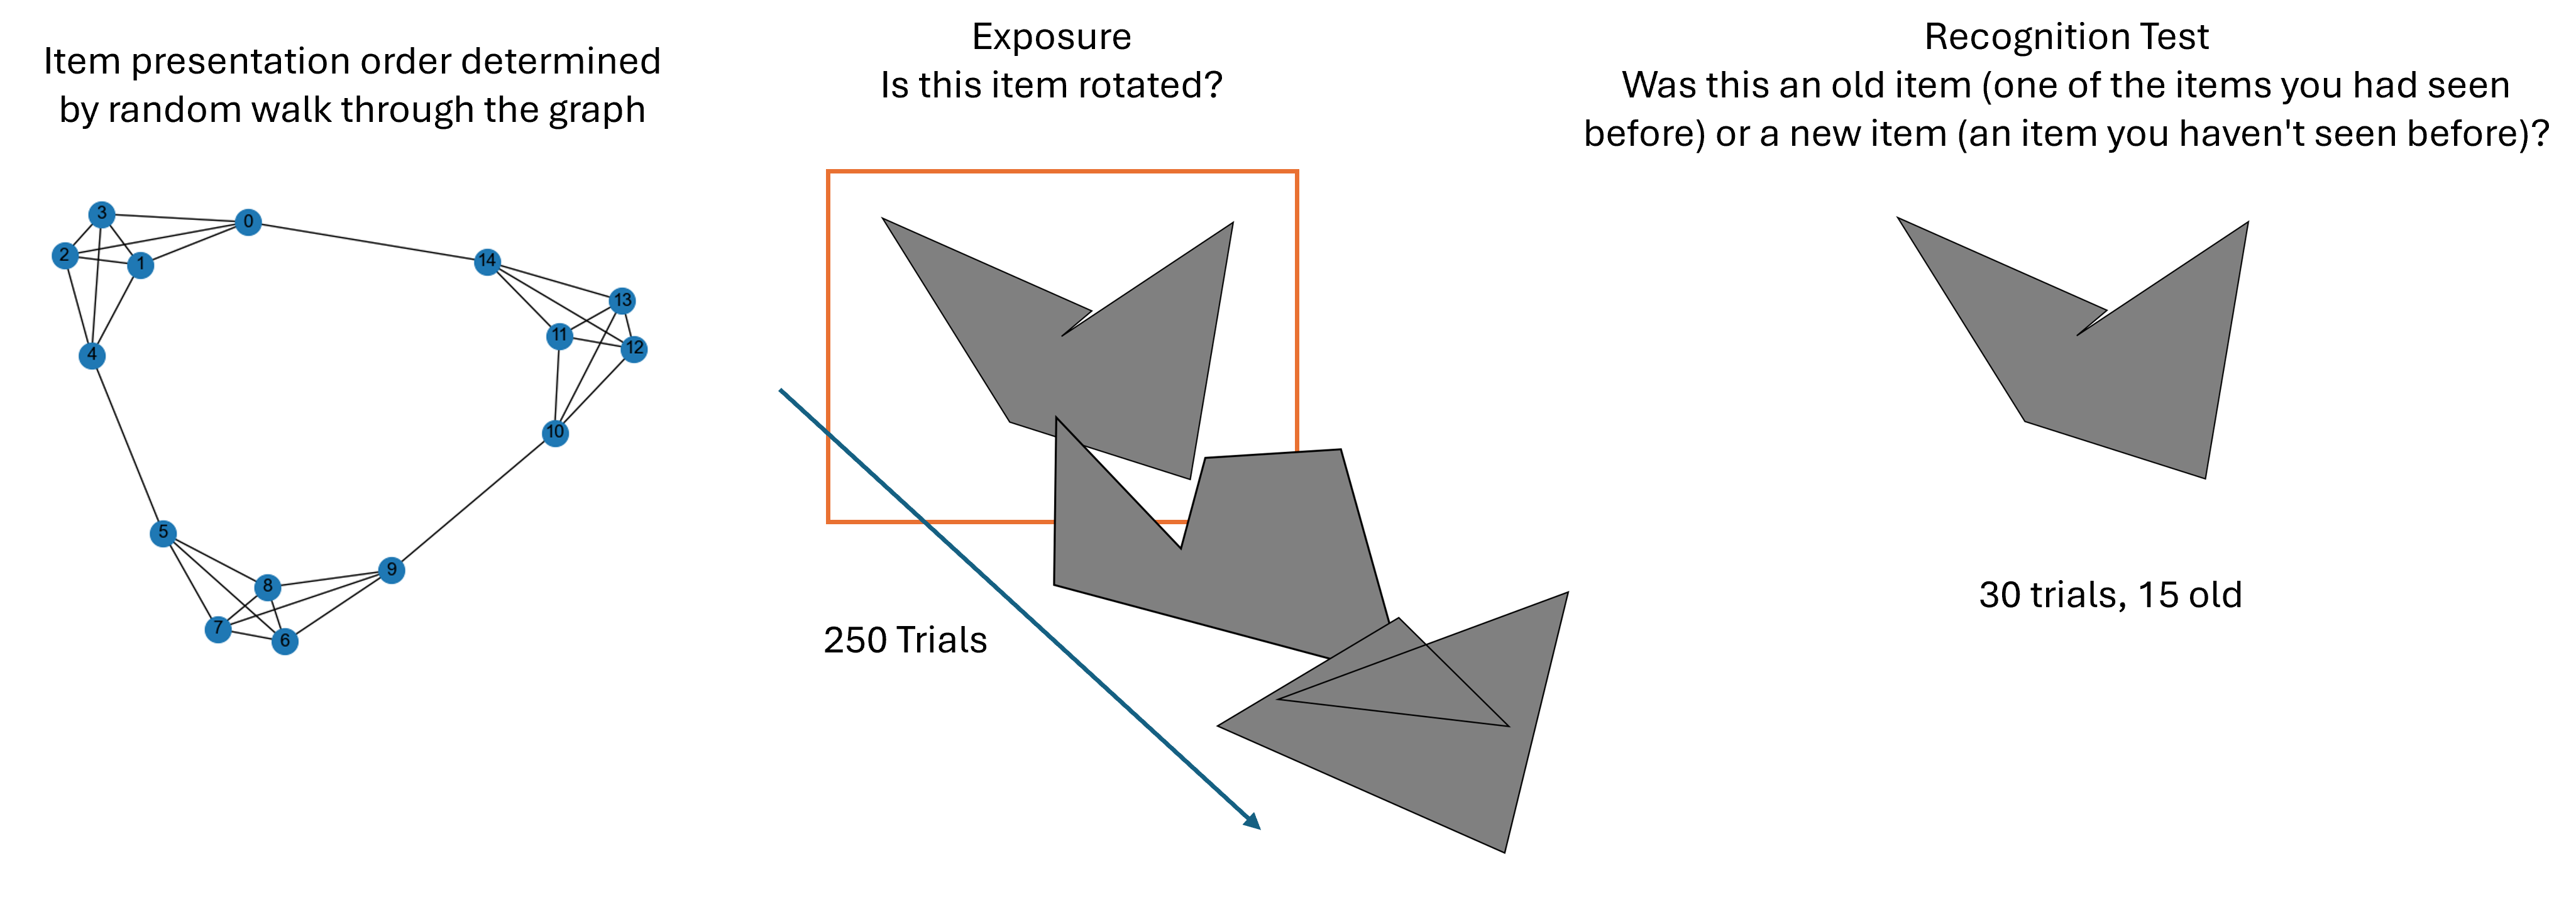
\includegraphics[width = \textwidth]{chapter_notebooks/chapter_3/figures/exp2_design.png}
    \caption{Design schematic for Experiment 2a. Three alternating blocks of exposure and recognition test were presented. A Stroop task was conducted prior to the final recognition test.}
\end{figure}

After each block of the exposure phase, participants went through a recognition memory test (Figure \ref{fig:exp2-design}). They were shown the 15 items they made rotation judgments on (in their canonical orientation) in addition to 15 new random polygon items and were asked to determine whether each of these items was old or new. Order of presentation of old and new items was randomized during the recognition memory test. Of the three recognition tests, the final test was conducted after a short Stroop task to washout any effects of short term memory. 

After the final recognition memory test, participants went through a source memory test. Each of the 15 studied items were shown without the colored borders that surrounded them during exposure. Participants were asked to choose which of the three colored borders, provided as on-screen options, surrounded any particular item. This source memory task was added to provide an additional signal for memory in case of ceiling effects of recognition memory tasks. However, no analyses have been done on this source memory task. 


\section{Results}
Table \ref{tab:exp2-rt-accuracy-stats} provides the means and standard deviations for response times and accuracies across each block for all stimuli types for both conditions. 
\begin{table}
    \centering
    \label{tab:exp2-rt-accuracy-stats}
    \caption{Accuracy and Response time Means and Standard Deviations for exposure and recognition phases in experiment 2}    
    \begin{tabular}{llllrrrr}
        \toprule
         &  &  &  & \multicolumn{2}{r}{accuracy} & \multicolumn{2}{r}{rt} \\
         &  &  &  & mean & std & mean & std \\
        phase & block & stimulus type & condition &  &  &  &  \\
        \midrule
        \multirow[t]{12}{*}{exposure} & \multirow[t]{4}{*}{0} & \multirow[t]{2}{*}{boundary} & structured & 0.683 & 0.465 & 1.644 & 1.911 \\
         &  &  & unstructured & 0.739 & 0.439 & 1.710 & 1.732 \\
        \cline{3-8}
         &  & \multirow[t]{2}{*}{nonboundary} & structured & 0.669 & 0.471 & 1.619 & 1.728 \\
         &  &  & unstructured & 0.728 & 0.445 & 1.713 & 1.689 \\
        \cline{2-8} \cline{3-8}
         & \multirow[t]{4}{*}{1} & \multirow[t]{2}{*}{boundary} & structured & 0.735 & 0.441 & 1.244 & 1.322 \\
         &  &  & unstructured & 0.796 & 0.403 & 1.283 & 1.243 \\
        \cline{3-8}
         &  & \multirow[t]{2}{*}{nonboundary} & structured & 0.739 & 0.439 & 1.250 & 1.343 \\
         &  &  & unstructured & 0.790 & 0.408 & 1.263 & 1.217 \\
        \cline{2-8} \cline{3-8}
         & \multirow[t]{4}{*}{2} & \multirow[t]{2}{*}{boundary} & structured & 0.757 & 0.429 & 1.168 & 1.657 \\
         &  &  & unstructured & 0.843 & 0.363 & 1.111 & 1.334 \\
        \cline{3-8}
         &  & \multirow[t]{2}{*}{nonboundary} & structured & 0.765 & 0.424 & 1.192 & 1.656 \\
         &  &  & unstructured & 0.838 & 0.369 & 1.085 & 1.546 \\
        \cline{1-8} \cline{2-8} \cline{3-8}
        \multirow[t]{18}{*}{memory} & \multirow[t]{6}{*}{0} & \multirow[t]{2}{*}{boundary} & structured & 0.796 & 0.404 & 1.681 & 1.490 \\
         &  &  & unstructured & 0.878 & 0.328 & 1.805 & 1.712 \\
        \cline{3-8}
         &  & \multirow[t]{2}{*}{new} & structured & 0.721 & 0.449 & 1.899 & 1.569 \\
         &  &  & unstructured & 0.782 & 0.413 & 1.770 & 1.666 \\
        \cline{3-8}
         &  & \multirow[t]{2}{*}{nonboundary} & structured & 0.782 & 0.414 & 1.715 & 1.602 \\
         &  &  & unstructured & 0.904 & 0.296 & 1.570 & 1.291 \\
        \cline{2-8} \cline{3-8}
         & \multirow[t]{6}{*}{1} & \multirow[t]{2}{*}{boundary} & structured & 0.833 & 0.374 & 1.564 & 2.573 \\
         &  &  & unstructured & 0.911 & 0.285 & 1.212 & 0.959 \\
        \cline{3-8}
         &  & \multirow[t]{2}{*}{new} & structured & 0.800 & 0.400 & 1.420 & 1.486 \\
         &  &  & unstructured & 0.873 & 0.333 & 1.338 & 1.056 \\
        \cline{3-8}
         &  & \multirow[t]{2}{*}{nonboundary} & structured & 0.860 & 0.348 & 1.618 & 1.812 \\
         &  &  & unstructured & 0.874 & 0.332 & 1.139 & 0.709 \\
        \cline{2-8} \cline{3-8}
         & \multirow[t]{6}{*}{2} & \multirow[t]{2}{*}{boundary} & structured & 0.907 & 0.291 & 1.196 & 1.194 \\
         &  &  & unstructured & 0.900 & 0.301 & 1.075 & 0.694 \\
        \cline{3-8}
         &  & \multirow[t]{2}{*}{new} & structured & 0.751 & 0.433 & 1.454 & 2.322 \\
         &  &  & unstructured & 0.844 & 0.363 & 1.292 & 1.127 \\
        \cline{3-8}
         &  & \multirow[t]{2}{*}{nonboundary} & structured & 0.893 & 0.310 & 1.370 & 1.869 \\
         &  &  & unstructured & 0.926 & 0.262 & 1.045 & 0.729 \\
        \cline{1-8} \cline{2-8} \cline{3-8}
        \bottomrule
        \end{tabular}
    \end{table}
        
As expected, accuracies for old stimuli increase with increased exposure (Figure \ref{fig:exp2-accuracies}) wheras the response times decreased with more experience with the stimuli across blocks (Figure\ref{fig:exp2-rts}). \footnote{Interestingly, overall accuracy of participants in the unstructured exposure condition is higher, than those in the structured exposure condition across all stimulus types. This effect may be due to participant variability.} 

\begin{figure}
    \centering
    \label{fig:exp2-accuracies}
    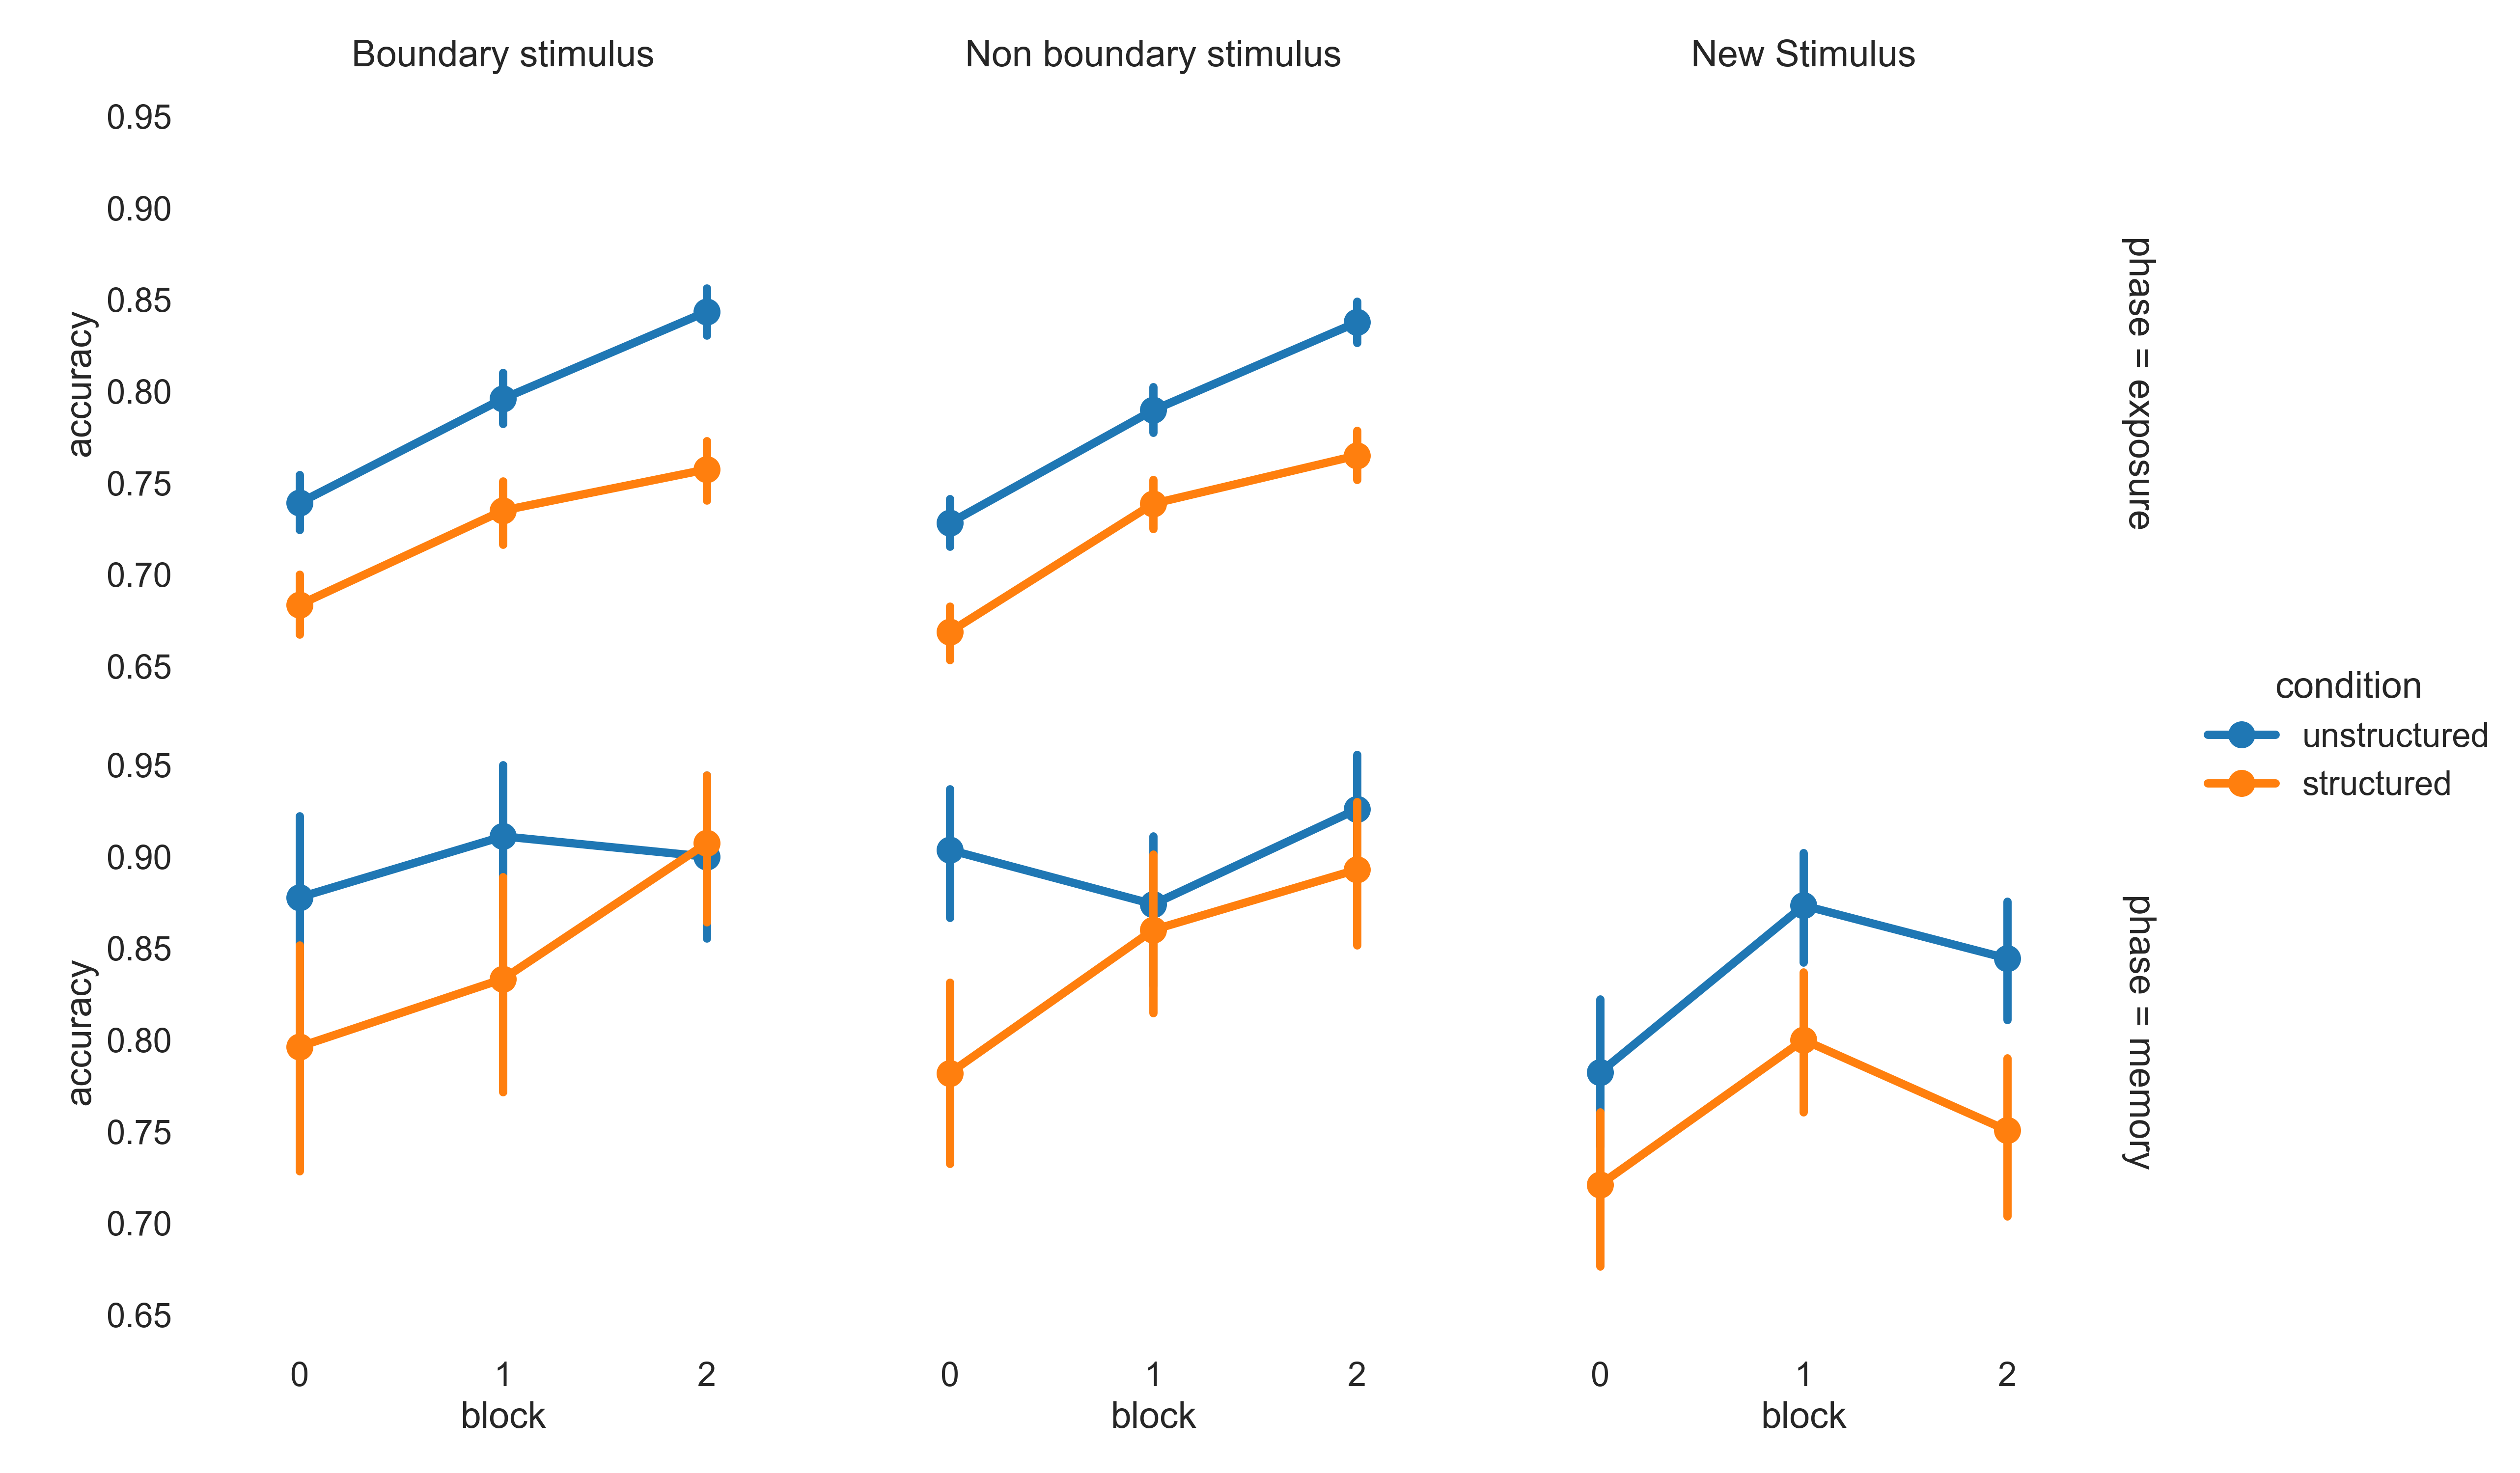
\includegraphics[width = \textwidth]{chapter_notebooks/chapter_3/figures/exposure_recog_accuracy_allphases.png}
    \caption{Mean accuracies for both participant groups (structured and unstructured) across blocks, for different stimulus types and phases of the experiment}
\end{figure}


\begin{figure}
    \centering
    \label{fig:exp2-rts}
    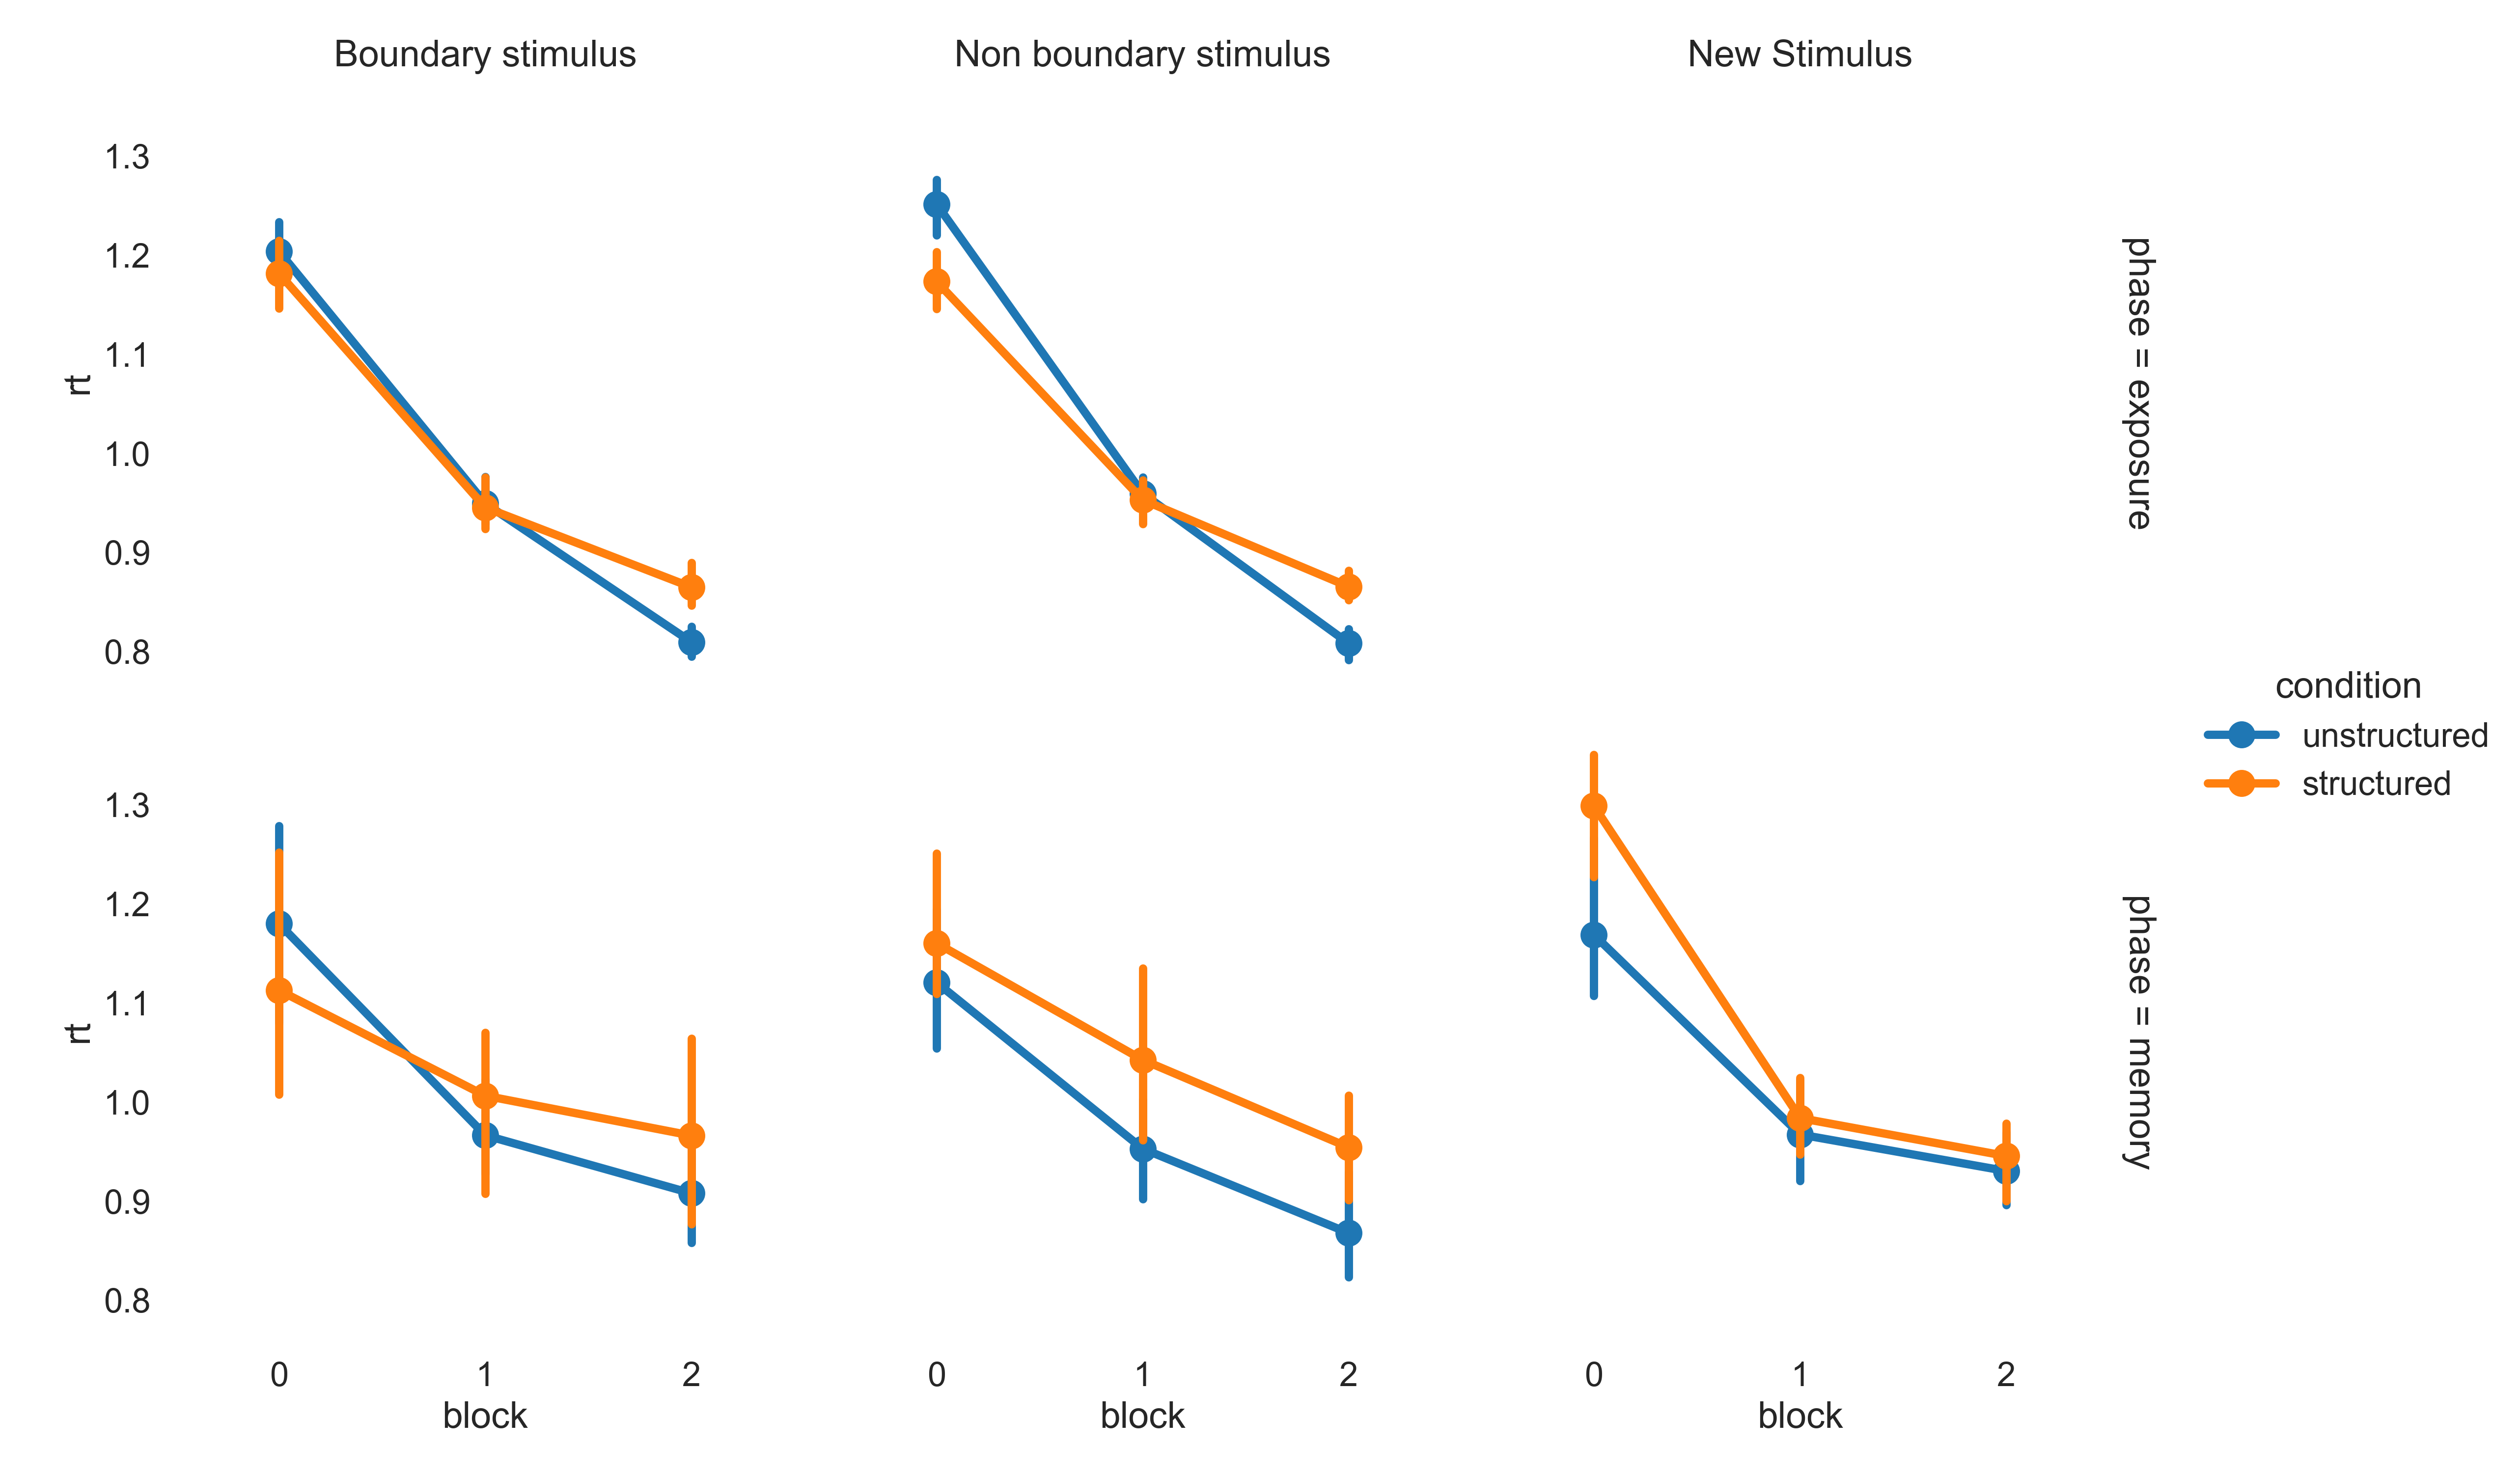
\includegraphics[width = \textwidth]{chapter_notebooks/chapter_3/figures/exposure_recog_rt_allphases.png}
    \caption{Median response times for both participant groups (structured and unstructured) across blocks, for different stimulus types and phases of the experiment}
\end{figure}

To assess differences between stimulus types (boundary vs non boundary) on recognition memory, a signal detection (SDT) model was first fit separately for boundary and non boundary items. The model for boundary items describes the probability of responding `old' to old boundary stimuli relative to new stimuli. Similarly, the model for non boundary items describes the probability of responding `old' to old non-boundary items relative to new stimuli. A participant intercept term allows for each participant to have their own decision criterion. Finally, accuracy at exposure was included as a factor in the SDT model. Exposure accuracy factor for old items was computed by averaging the rotation judgment accuracy for each of the old items in the block immediately before the recognition memory block. For new items, this factor was computed by averaging the rotation judgment accuracy for all exposure items in the exposure block before that recognition phase. The model fits relatively well as shown in figure \ref{fig:exp2-sdt-fits}.

\begin{figure}
    \centering
    \label{fig:exp2-sdt-fits}
    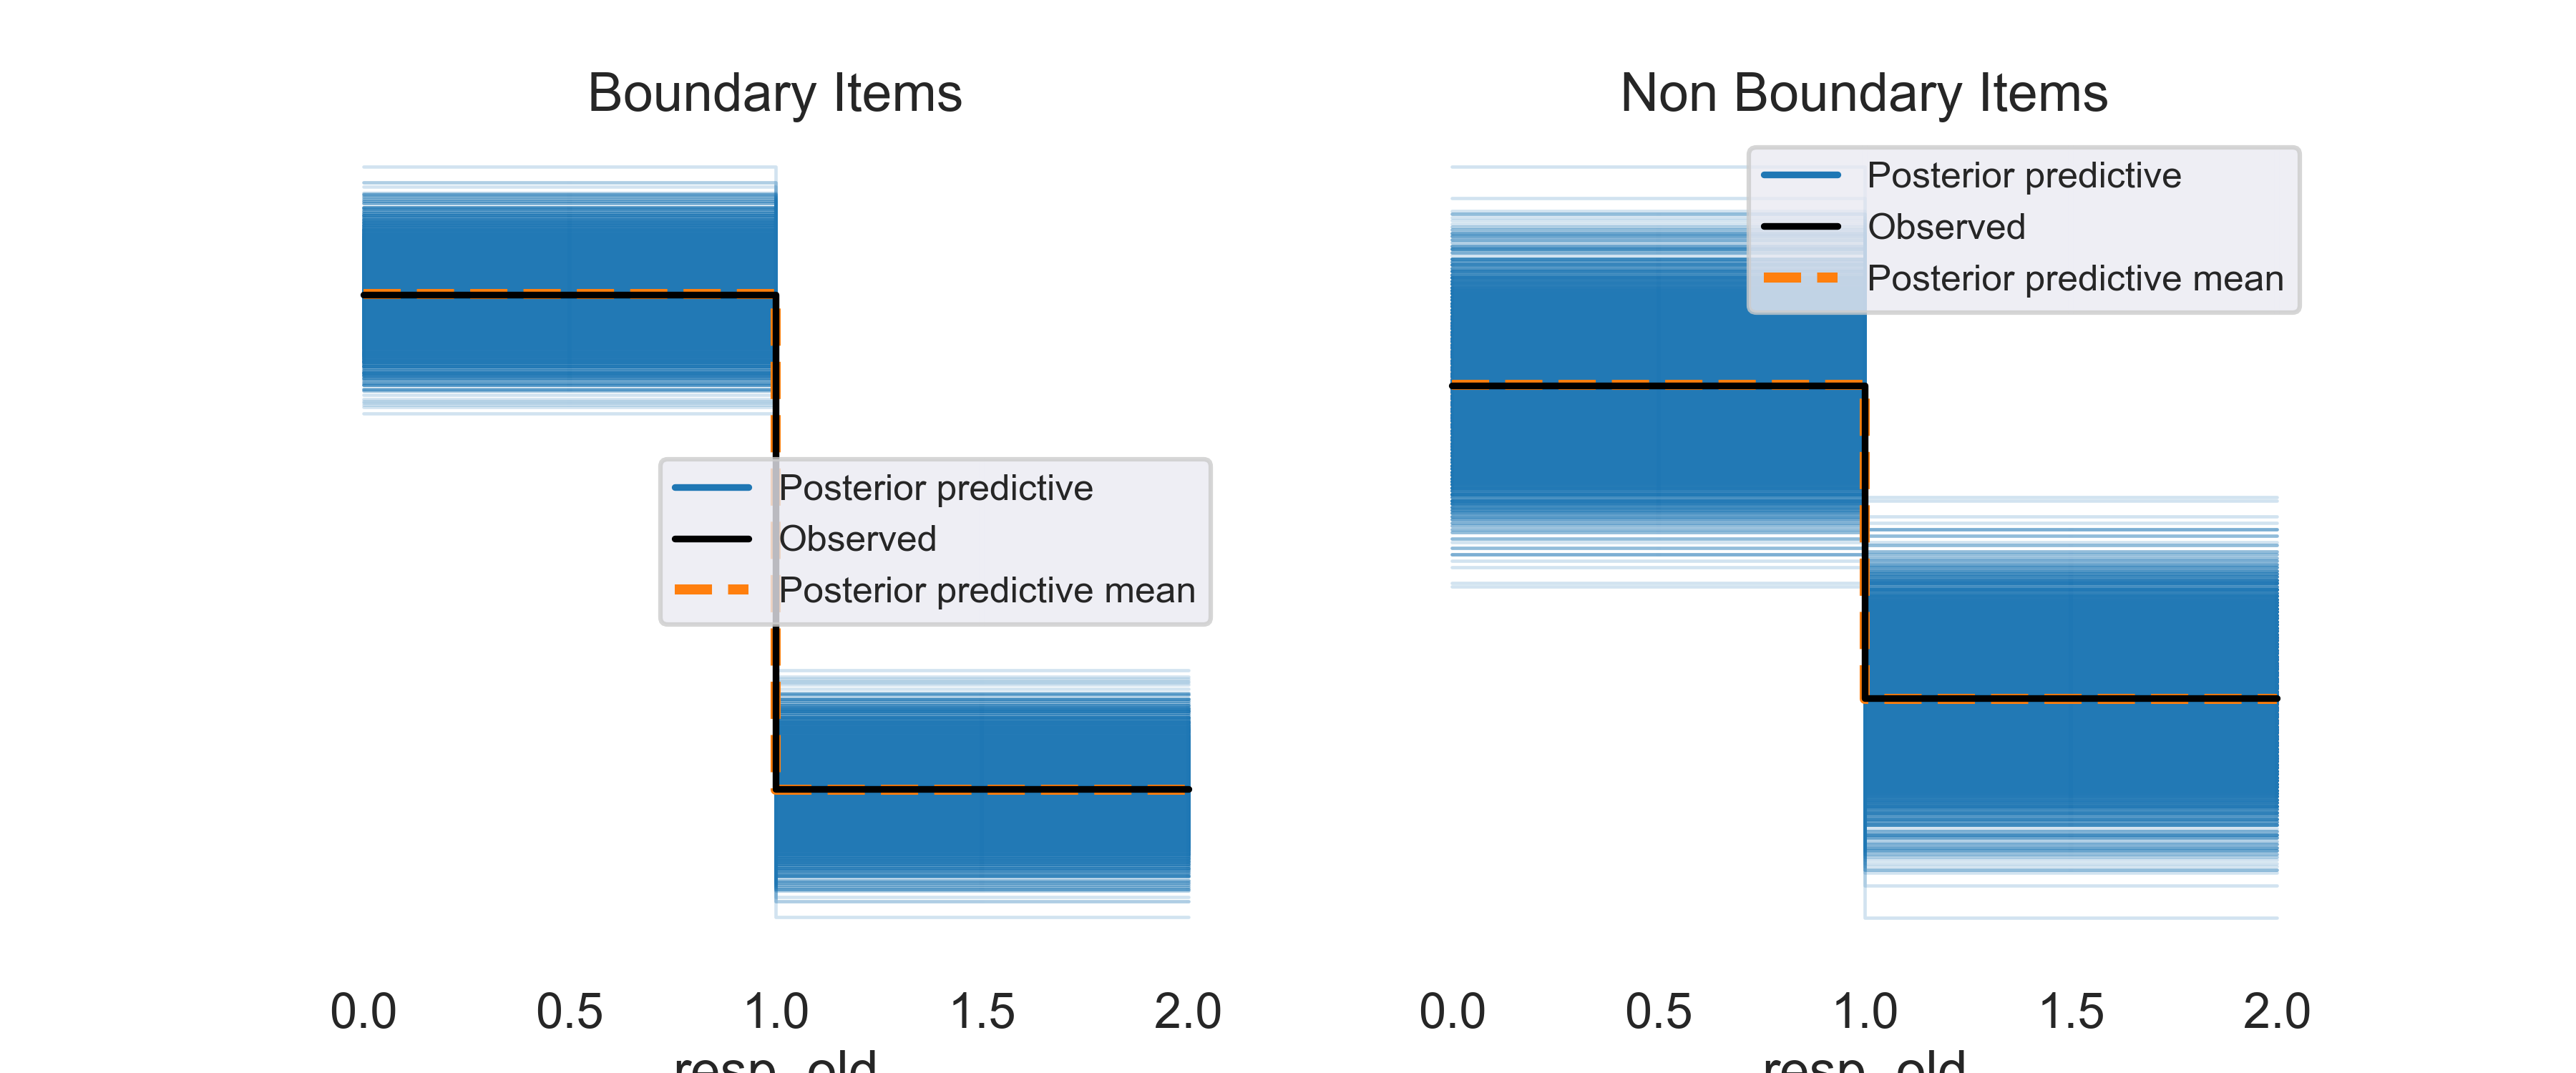
\includegraphics[width = \textwidth]{chapter_notebooks/chapter_3/figures/ppc_sdt_model.png}
    \caption{SDT Model Posterior Predictive Distributions for boundary and non boundary items}
\end{figure}

$d'$ measures the distance between distributions of old and new items. Parameter estimates of $d'$ for structured relative to unstructured for boundary and non boundary nodes for the final recognition block are shown in figure \ref{fig:sdt-params}. Parameter statistics are reported in appendix tables \ref{tab:exp3-bayesmodel-boundary-sdt} and \ref{tab:exp3-bayesmodel-nonboundary-sdt}

\begin{figure}
    \centering
    \label{fig:sdt-params}
    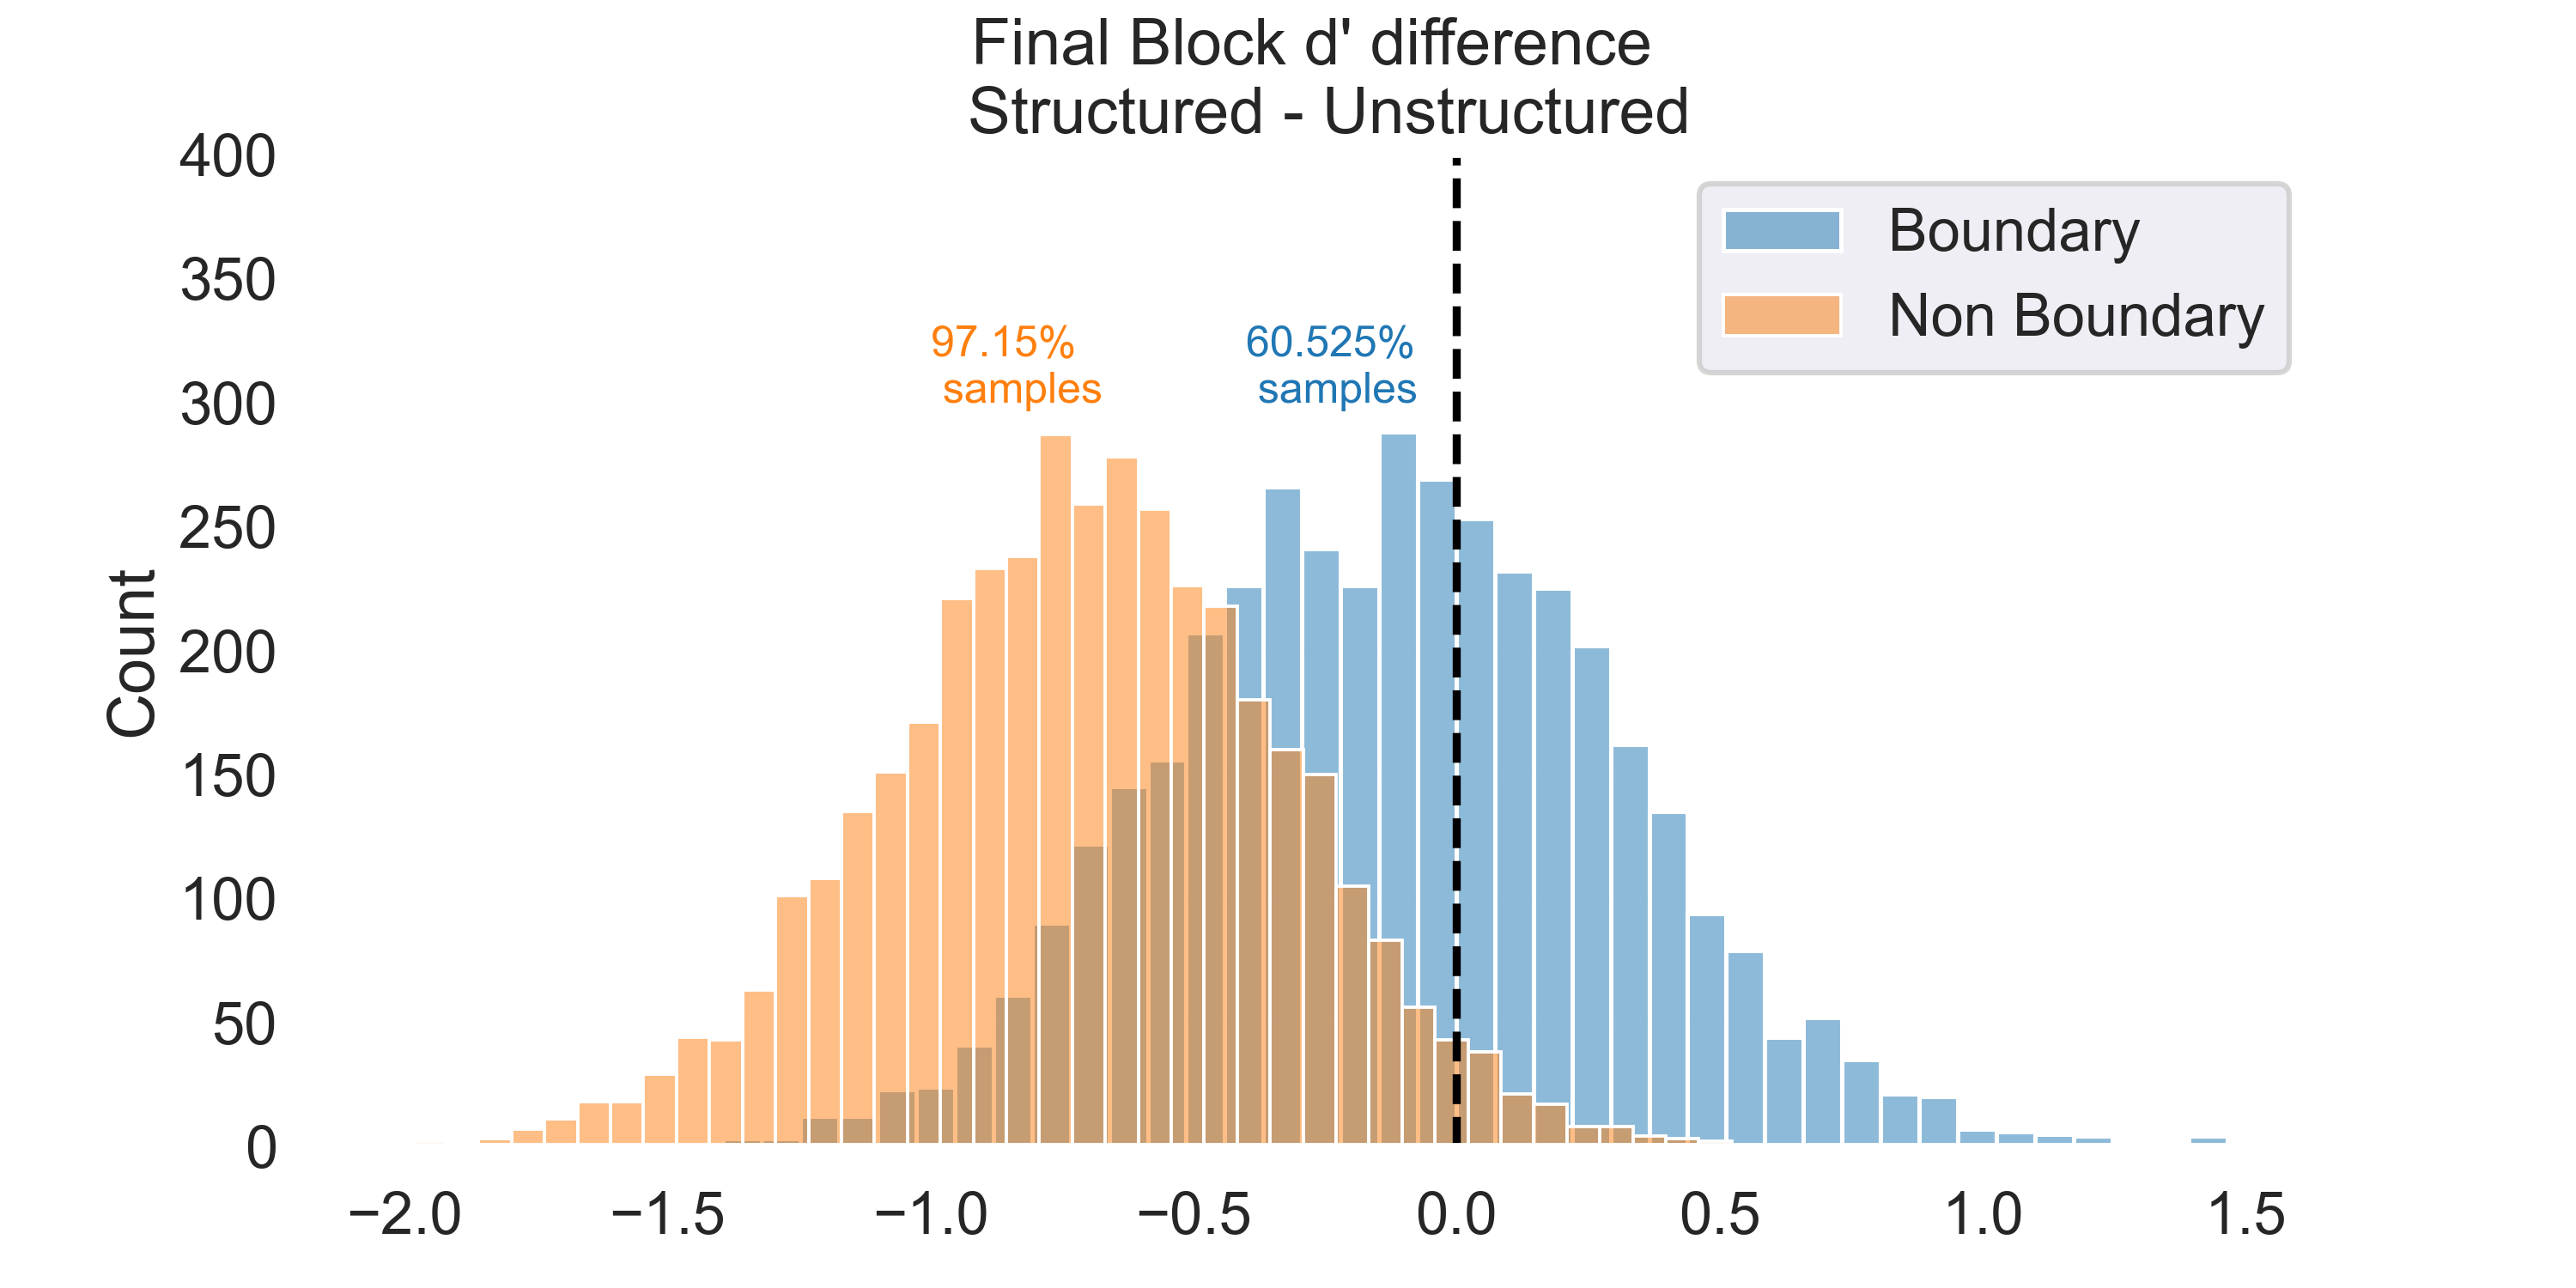
\includegraphics[width = \textwidth]{chapter_notebooks/chapter_3/figures/sdt_d_results.png}
    \caption{Differences in $d'$ for models fit to separately boundary and non boundary nodes for both structured and unstructured exposure conditions}
\end{figure}

The SDT modeling implies that while there are no differences in recognition memory for boundary nodes based on exposure, non boundary nodes become less recognizable under structured exposure condition. However, 

\subsection*{Diffusion Modeling}
However, the model used above fails to account for ceiling effects -- accuracy for old items is near perfect or could have reached an asymptote. Those models also do not account for encoding accuracy during exposure -- participants may fail to recognize old items if they did not study those items well as indicated by the rotation judgement task. Models were also fit separately to derive $d'$ for boundary and non-boundary items, thus losing shared variability within the participant.

To be able to account for both ceiling effects and effects of exposure, we can use additional information available in form of response times during the recognition memory task. For example, for participants equally accurate in recognizing boundary and non-boundary participants, being able to recognize boundary items faster may provide additional evidence for better memorability of these items relative to slower recognized non-boundary items. Figure \ref{fig:recognition-rts} shows median response times across three blocks of recognition test. 

To understand recognition memory differences between boundary and non-boundary items in context of response accuracy and response time distributions, we use the Drift Diffusion Model \(DDM\). The DDM, which falls under a class of sequential sampling models, has been a widely successful model in modeling two-choice tasks in recognition memory \cite{ratcliff2004diffusion, ratcliff2022discriminating, starns2014using, starns2014validating, ratcliff2009modeling}. The function of the DDM is depicted in Figure \ref{fig:ddm-model}. 

\begin{figure}[ht]
    \label{fig:ddm-model}
    \centering
    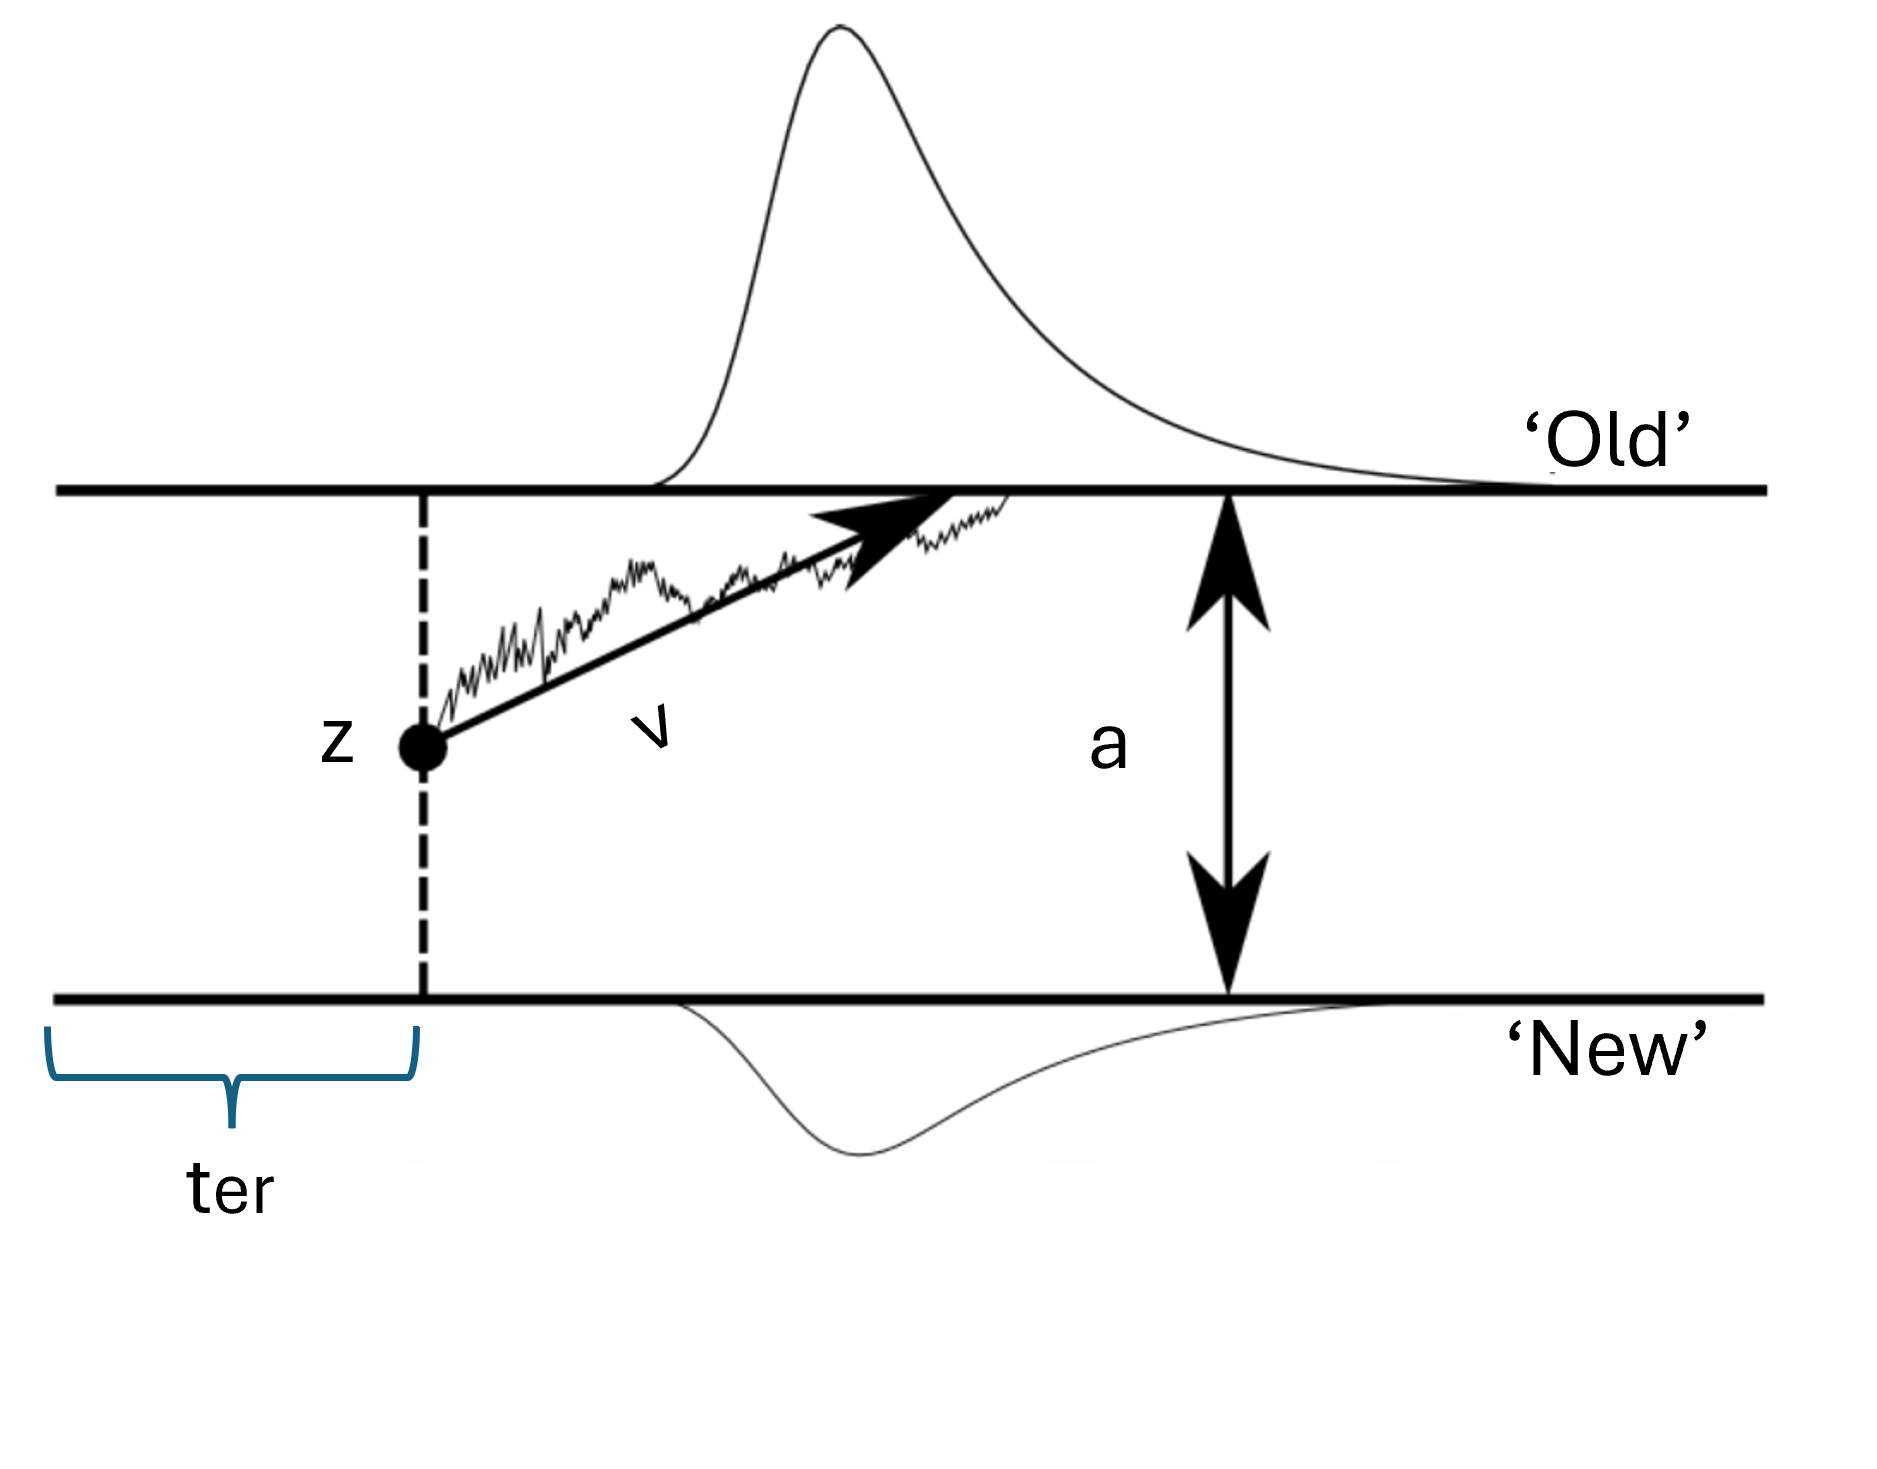
\includegraphics[width = 0.75\textwidth]{chapter_notebooks/chapter_3/figures/ddm.png}
    \caption{The Drift Diffusion Model of Choice Response Times for Old/New recognition memory tasks.}
\end{figure}

Briefly, the DDM assumes that at choice time, evidence from two presented options accumulates sequentially over time towards one of the two boundaries. For a previously studied item presented at test, the evidence from the item accumulates slowly towards the `old' boundary whereas for a non-studied item, the evidence accumulates towards the `new' boundary. The rate of evidence accumulation is controlled by the drift rate parameter, `$v$'. Participants may be biased towards making an old or a new response at test; this bias is measured by the starting point parameter, `$z$'. THe boundary separation between the two responses is modeled by a parameter `$a$'. Finally, the observed response consists of cognitive processes not affiliated with decision making (such as time it takes to visually process the test item, time for the motor systems to click the relevant key) which are modeled by a non-decision time parameter `$t_{er}$'. \footnote{Note that this version of the DDM is a simplified model. More complex DDMs account for trial-to-trial variability in each parameters as well.} 

Prior work has shown that memory strength of previously studied items impacts the drift rate towards old/new responses. The drift rate parameter implies that a stronger match to memory leads to a quicker accumulation of evidence towards the `old' response boundary. Similarly, a stronger mis-match to memory allows for a quicker accumulation of evidence towards the `new' response boundary\cite{ratcliff2004diffusion,ratcliff2022discriminating}. 

The DDM thus allows us circumvent ceiling effects by modeling response time distributions and estimate whether if boundary items are indeed a remembered better than non-boundary items in the structured exposure or whether the effect is driven by worse-remembered non-boundary items. 

For the recognition task in the current study, the DDM was parameterized as follows: 
\begin{equation}
    \begin{aligned}
        v \sim 0 + node type:condition:block + accuracy exposure \\
        z \sim 0 + block \\
        a \sim 0 + condition:block \\
        t = 0.25
    \end{aligned}
\end{equation}

The fixed value of the non decision time parameter $t$ was derived by first fitting the DDM over a range of possible $t$ values (i.e. a grid search) and picking value with the best fitting model in that range. DDM models were fit using the HSSM package \cite{fengler2022beyond}. \footnote{Unfortunately the non decision time parameter is too difficult to fit -- this is a known problem with the HSSM package} 

\subsubsection*{DDM Results}
The modeling framework above allows incorporating response times during recognition memory tasks. In particular, if an item has quickly and accurately recognized as old or new, in addition to good accuracy, such recognition would result into faster reaction times. This effect is captured by the drift rate parameter of the DDM. 

\begin{figure}
    \centering
    \label{fig:ddm-drift-rates}
    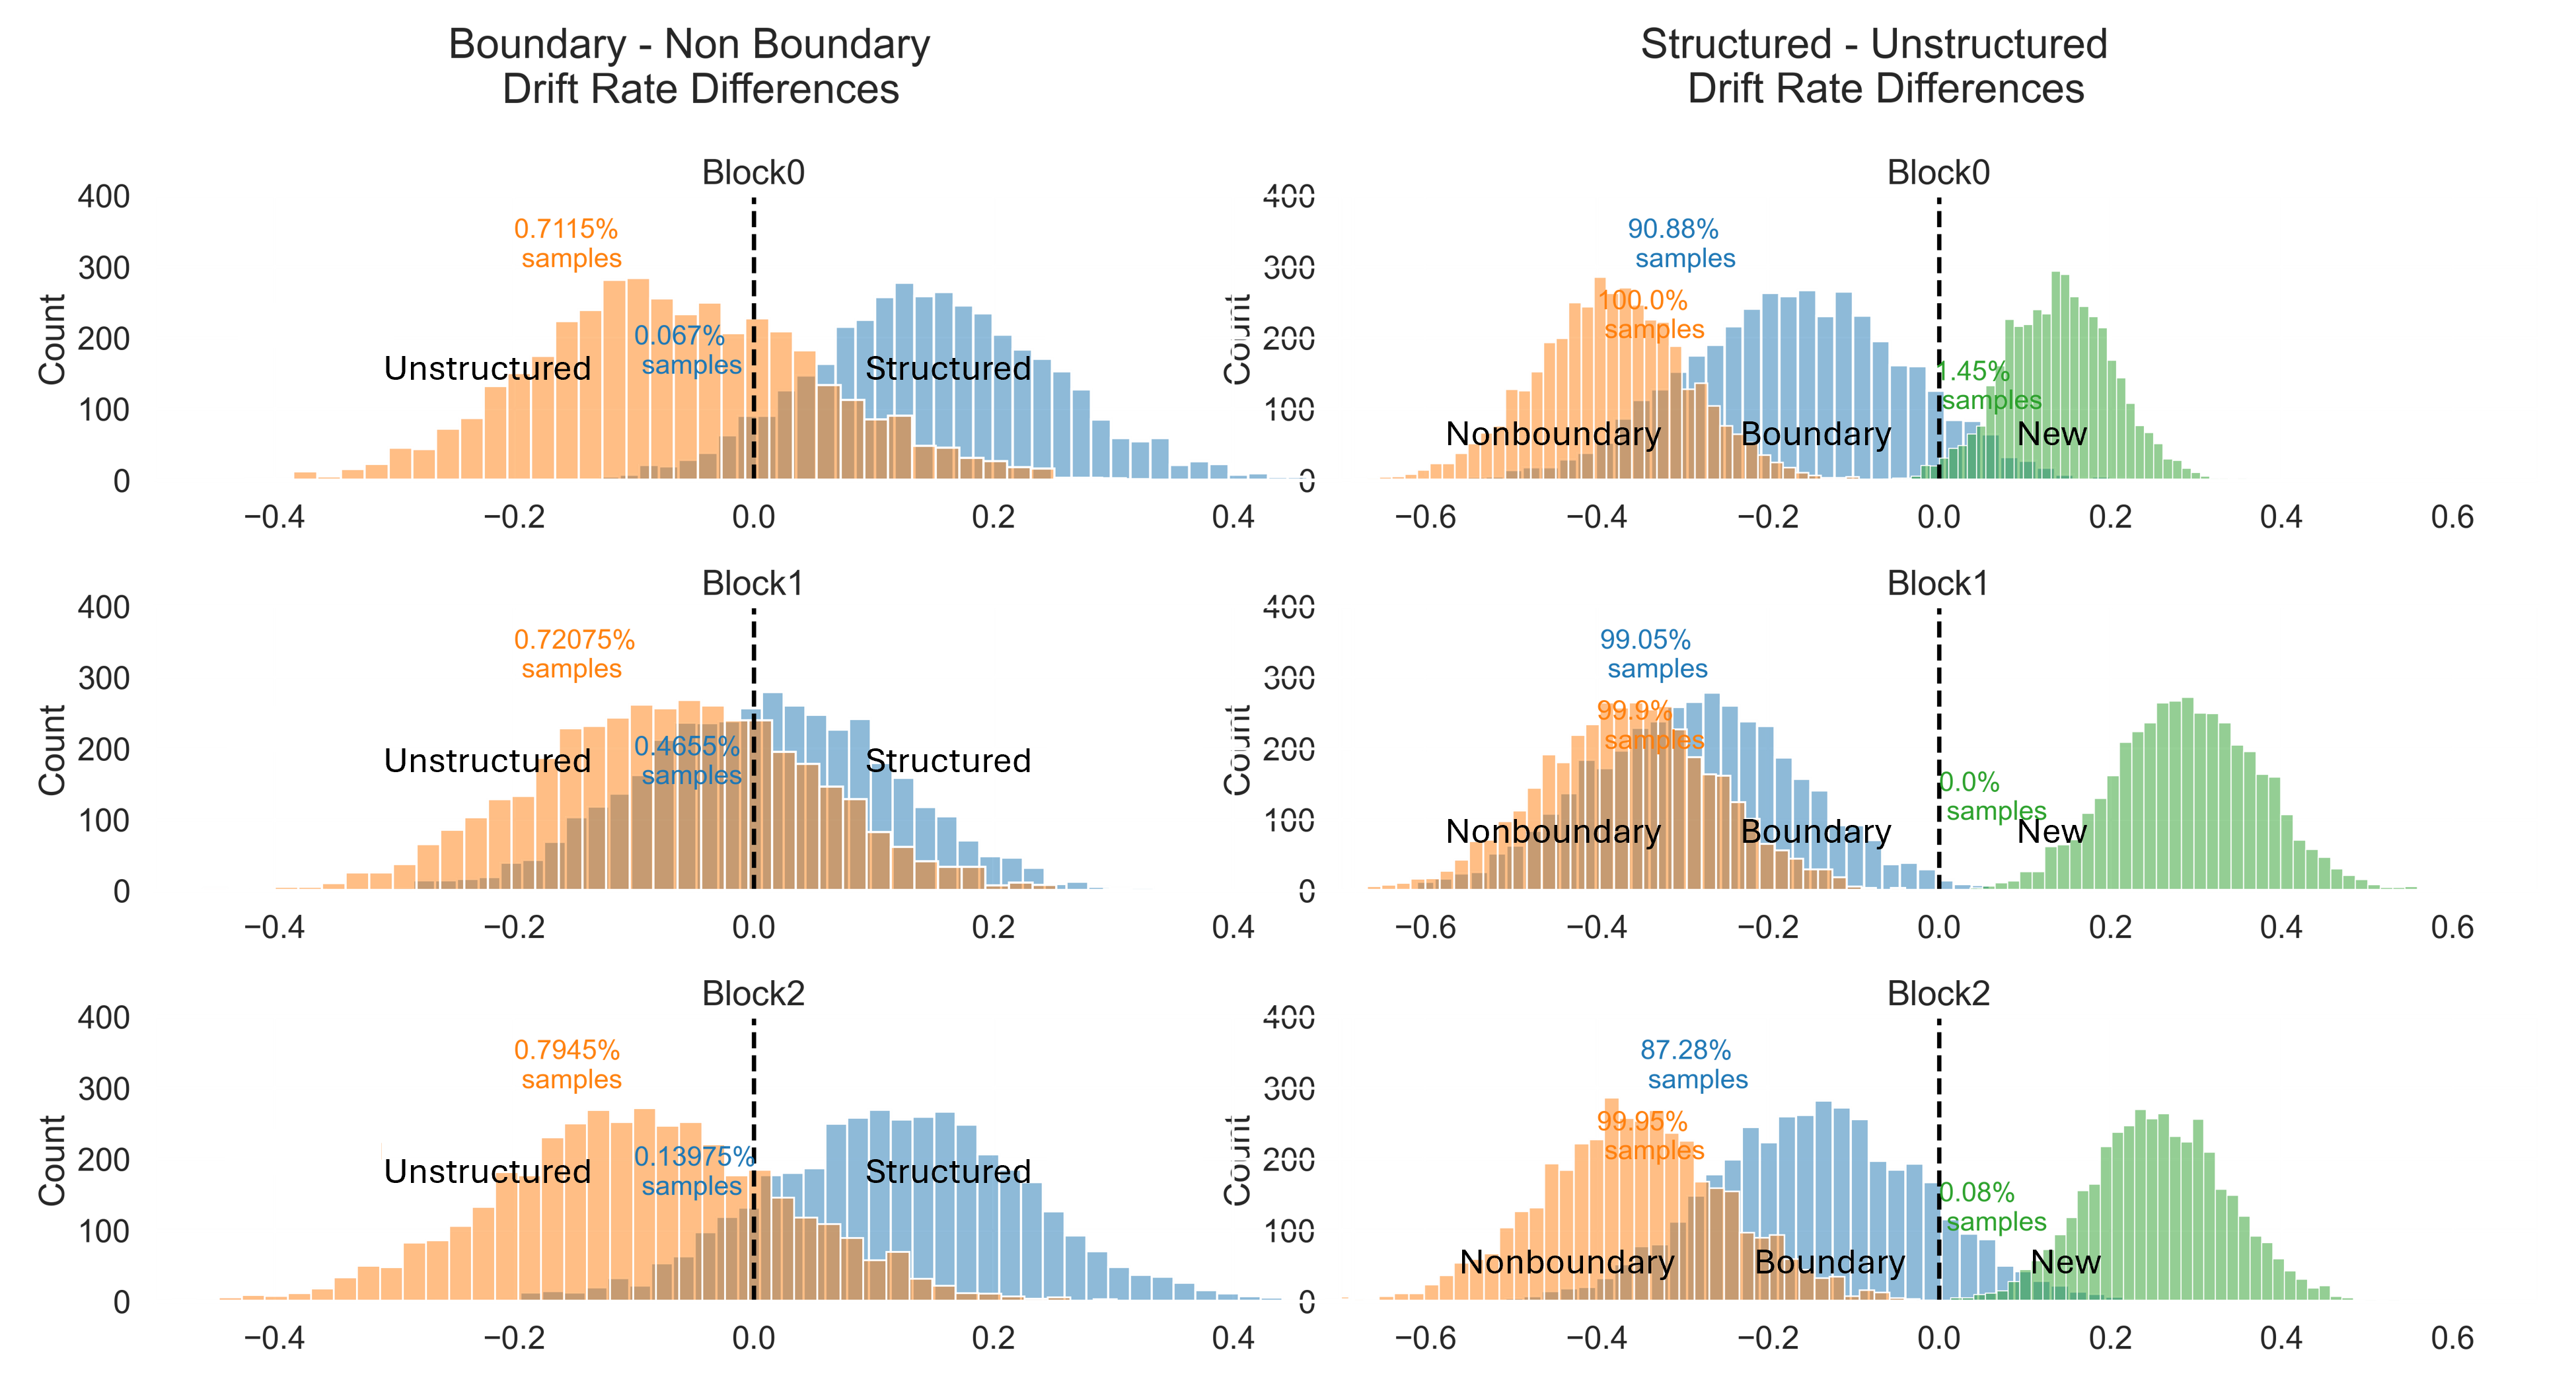
\includegraphics[width = \textwidth]{chapter_notebooks/chapter_3/figures/ddm_vdiff_comb.png}
    \caption{Drift rate differences. \textit{Left Panel.} Differences between boundary and non boundary nodes for structured and unstructured exposure conditions. \textit{Right Panel} Differences between drift rates between structured and unstructured conditions for each type of recognition memory stimulus. Figure text over each difference distribution depicts the proportion of posterior samples below 0.}
\end{figure}

Figure \ref{fig:ddm-drift-rates} shows the differences between drift rate parameters. The left panel shows that boundary nodes have a higher drift rate than non boundary nodes in the structured conditions relative to the unstructured conditions. The right panel shows the same effect within conditions. New items appear to have better drift rates than old items in the structured condition than the unstructured conditions. Finally, all drift rate differences are the lowest in the middle block indicating improved memory after 500 trials of exposure to the same stimuli relative to 250 trials after the first block. Increased differences in after the final block are likely owed to the Stroop distracter task prior to the final recognition test. 



\section{Modeling Boundary Distance Effects}
Another replicated finding in explicitly operationalized event boundary literature is an apparent increased separation of events across boundaries \cite{horner2016role,brunec2018boundaries,dubrow2013influence, ezzyat2011constitutes, heusser2018perceptual}. This separation of events across boundaries helps shape narratives in long term memory \cite{clewett2019transcending}.

It is unknown, however, whether the increased temporal separation across event boundaries generalizes to boundaries operationalized implicitly as well. Context models such as SR provide a mechanism to directly estimate perceived distance between events. Specifically, each cell in the SR matrix $M(s, s')$ indicates the future expected visit probabilities from state $s$ to state $s'$. Under the assumption that states closer to the current state are visited more often in a random walk than state farther, the probability $M(s, s')$ provides a direct estimate of perceived distance from node $s$ to $s'$. 

\begin{figure}[ht]
    \centering
    \label{fig:two_module_graph}
    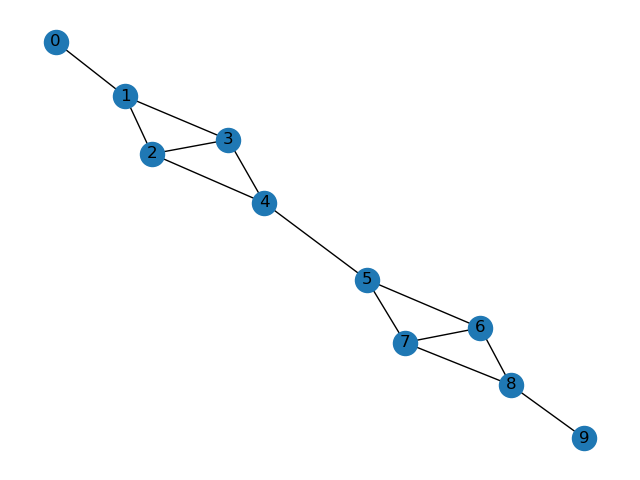
\includegraphics[width = \textwidth]{chapter_notebooks/chapter_3/figures/two_module_graph.png}
    \caption{Two module graph used for distance judgments.}
\end{figure}

To test whether cross boundary events are perceived to be farther from each other relative to within-boundary events graph in figure \ref{fig:two_module_graph} is used. The key transitions of interest that are compared in this graph are transitions at equal distances. Below I specify example transitions at 3 different distances however, for simulations and the experiment, all symmetrical transitions at those distances were tested. 
\begin{itemize}
    \item $0 \leftrightarrow 4$ vs $1 \leftrightarrow 5$ at shortest distance 3. 
    \item $1 \leftrightarrow 4$ vs $2 \leftrightarrow 5$ at shortest distance 2. 
    \item $2 \leftrightarrow 4$ vs $4 \leftrightarrow 4$ at shortest distance 1. 
\end{itemize}

\begin{figure}
    \centering
    \label{fig:SR-distance-estimate}
    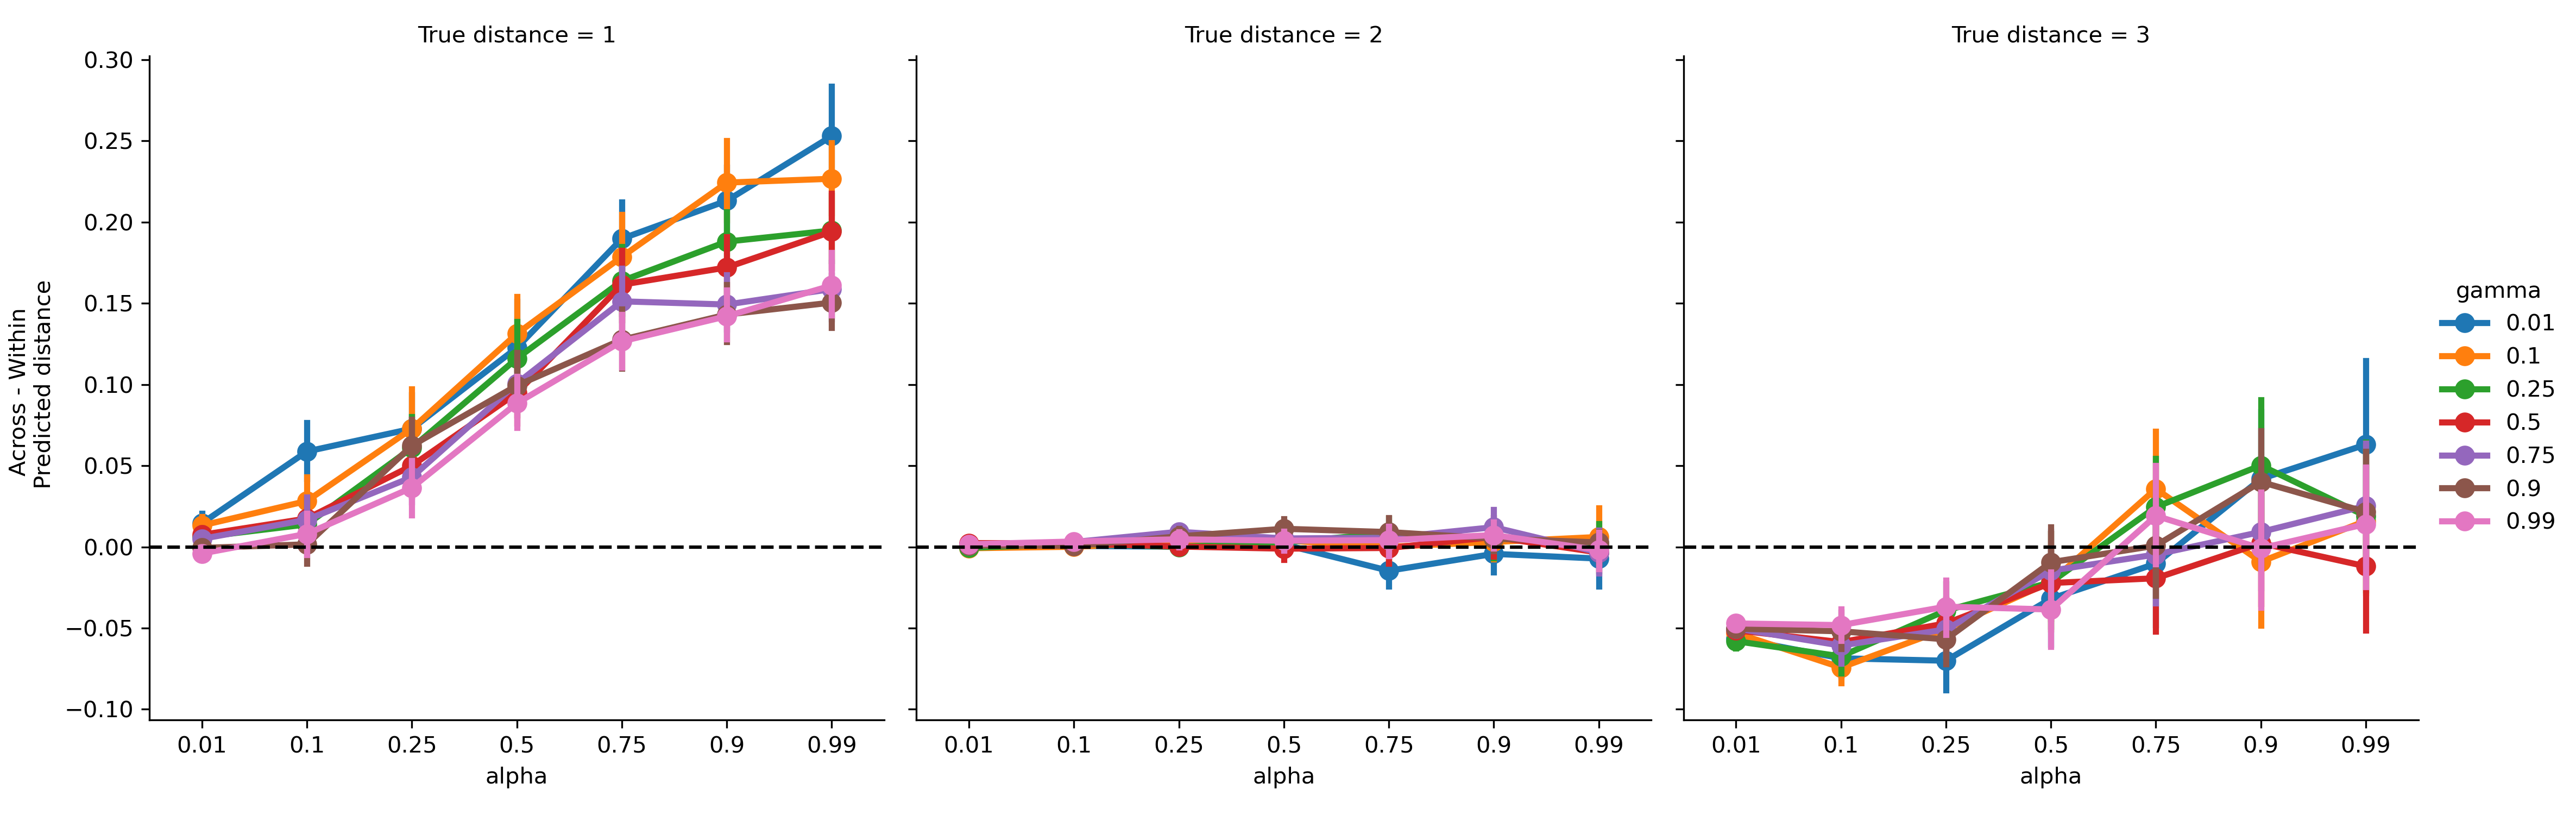
\includegraphics[width = \textwidth]{chapter_notebooks/chapter_3/figures/distance_predictions.png}
    \caption{SR predictions of distances across boundaries relative to distances within boundaries for nodes at true distance of 1, 2, and 3 and different parameter combinations.}
\end{figure}

SR estimate of distances is shown in figure \ref{fig:SR-distance-estimate}. Simulations predict that while boundary nodes themselves get perceptually farther with increased discount rate, neither of node-pairs at distance 2 or 3 that involve boundary nodes reliably show an increased cross-cluster distance.

\begin{figure}
    \centering
    \label{fig:SR-distance-estimate-entropy-boost}
    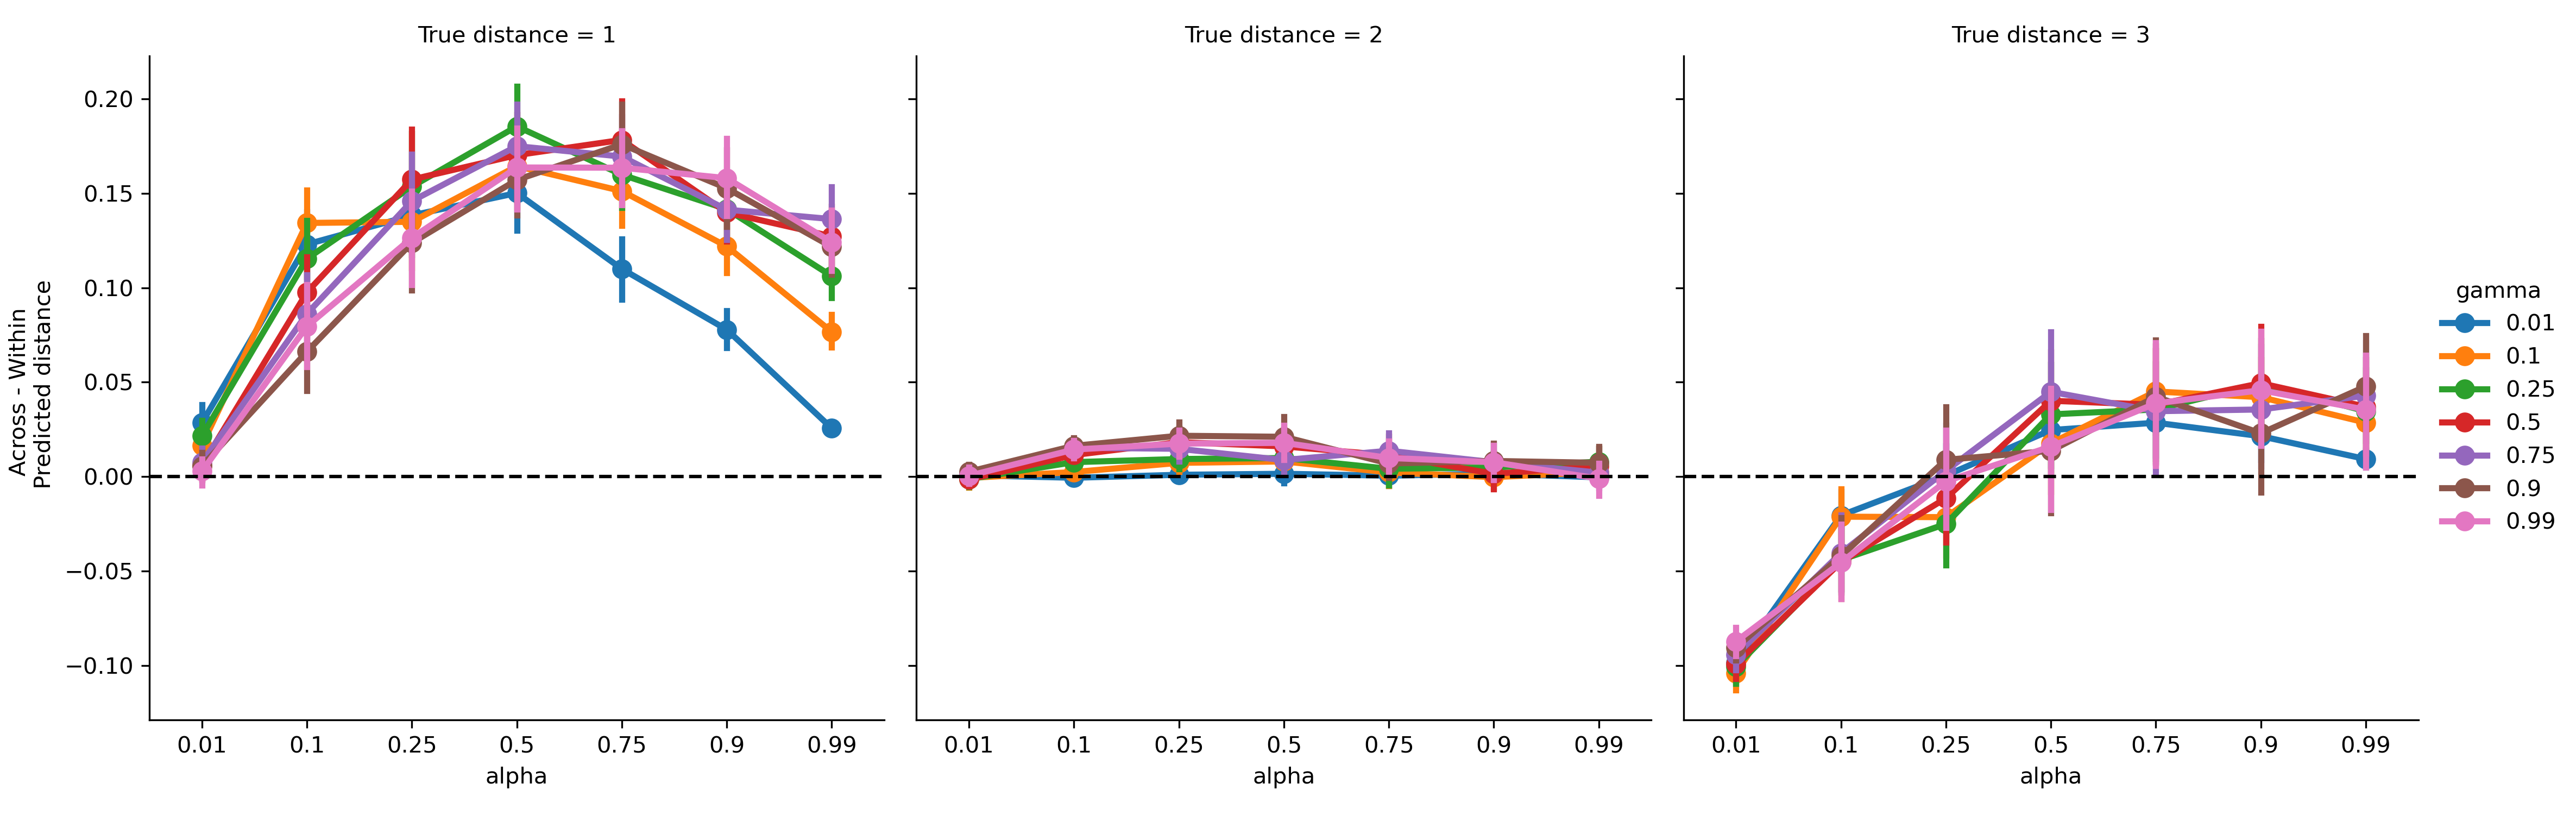
\includegraphics[width = \textwidth]{chapter_notebooks/chapter_3/figures/distance_predictions_entropyboost.png}
    \caption{SR predictions of distances across boundaries when boosted by node entropies relative to distances within boundaries for nodes at true distance of 1, 2, and 3 and different parameter combinations.}
\end{figure}

However, in a typical experience of the random walk, participants are shown to be slow at responding to boundary nodes; both due to higher entropy at boundary nodes (from chapter \ref{chapter-2-walk-lengths-modulate-statistical-learning}) and previously shown increased response times during transitions across temporal clusters \cite{lynn2020abstract,kahn2018network}. On average, a participant would typically spend more time at boundary nodes than non-boundary nodes thereby leading; thereby leading to increased perceived \textit{time} while crossing boundary nodes relative to staying within the cluster. Following the findings in chapter \ref{chapter-2-walk-lengths-modulate-statistical-learning}, this increased perceived time can be modeled through entropy difference between boundary and non-boundary nodes based on learned SR representations. This slowdown is simulated by multiplying average SR entropy of boundary nodes where they transitions cross boundaries and by multiplying the average SR entropy of non-boundary nodes where transitions stay within a cluster. predictions of differences in perceived distance are shown in figure \ref{fig:SR-distance-estimate-entropy-boost}.


Regardless of whether the distance measure is boosted by increased entropy at boundary nodes, it appears that boundary nodes themselves appear farther from each other relative to nodes within a cluster from that cluster's boundary node. Model predictions at other distances are mixed and dependent on parameters of the SR model. The next experiment tests whether the typical finding of increased perceived separation between cross cluster nodes (relative to within cluster nodes) is replicated in implicitly operationalized event boundary paradigms. A rigorous test of this formulation of the SR model is out of the scope of this dissertation. Furthermore, a lack of increased cross-cluster distance will provide no evidence for or against the current formulation of the SR model's role in representing distances between nodes. However, if such an increased cross-cluster distance is found, such an effect will serve as evidence \textit{against} the current formulation of the SR model's role in estimating temporal distances. 

\subsection{Methods}
\subsubsection*{Participants}
45 undergraduate students at the University of Massachusetts Amherst participated in this study. Participants were at least 18 years of age and were compensated via course credit. All study procedures were approved by the University Institutional Review Board. 

\subsubsection*{Design and Procedures}
Participants were randomly assigned to either a structured exposure or an unstructured exposure group. The overall experimental procedures were the same across both groups. 

Participants were first introduced to 10 randomly generated polygons and informed that these polygons are in their canonical orientation. Participants were asked to study these carefully and informed that they will make judgments about the orientation of these polygons in the coming phase. During the exposure phase, participants were shown one polygon at a time from the set of 10 they were introduced to. On each trial, the polygon was either rotated by 90 degrees or shown in its canonical orientation. Participants were asked to judge whether the polygon is rotated or not. 

The order of trials in exposure phase was determined based on a participant's group. 27 participants in the structured exposure condition were exposed to a stimulus stream generated by a random walk through the graph in figure \ref{fig:two_module_graph}. 18 participants in the unstructured exposure condition were shown a stimulus stream generated by randomly choosing any of the 10 polygons to be shown on any trial. The exposure phase lasted for 300 trials or 30 minutes, whichever came first. Participants were provided with an opportunity to take a self-paced break after 150 trials. 

During the test phase, participants were shown a triplet of polygons (see figure \ref{fig:exp3-design}). For each top polygon, participants were asked which of the bottom polygons was likely to appear first after seeing the polygon at the top in the stream they had experienced during exposure. The distance judgment phase lasted for 20 trials where 10 trials were consisted of the critical pairs (examples listed in the previous section) and 10 filler trials were based on randomly generated (non repeated) triplets. Responses to these filler trials were not analyzed.

\subsection{Results}

Figure \ref{fig:exp3-choice-results} provides an overview of the proportion of choices participants made to indicate a within cluster item is closer to the top item than a between cluster item. Descriptive statistics in table \ref{tab:exp3-choice-stats}

\begin{figure}
    \centering
    \label{fig:exp3-choice-results}
    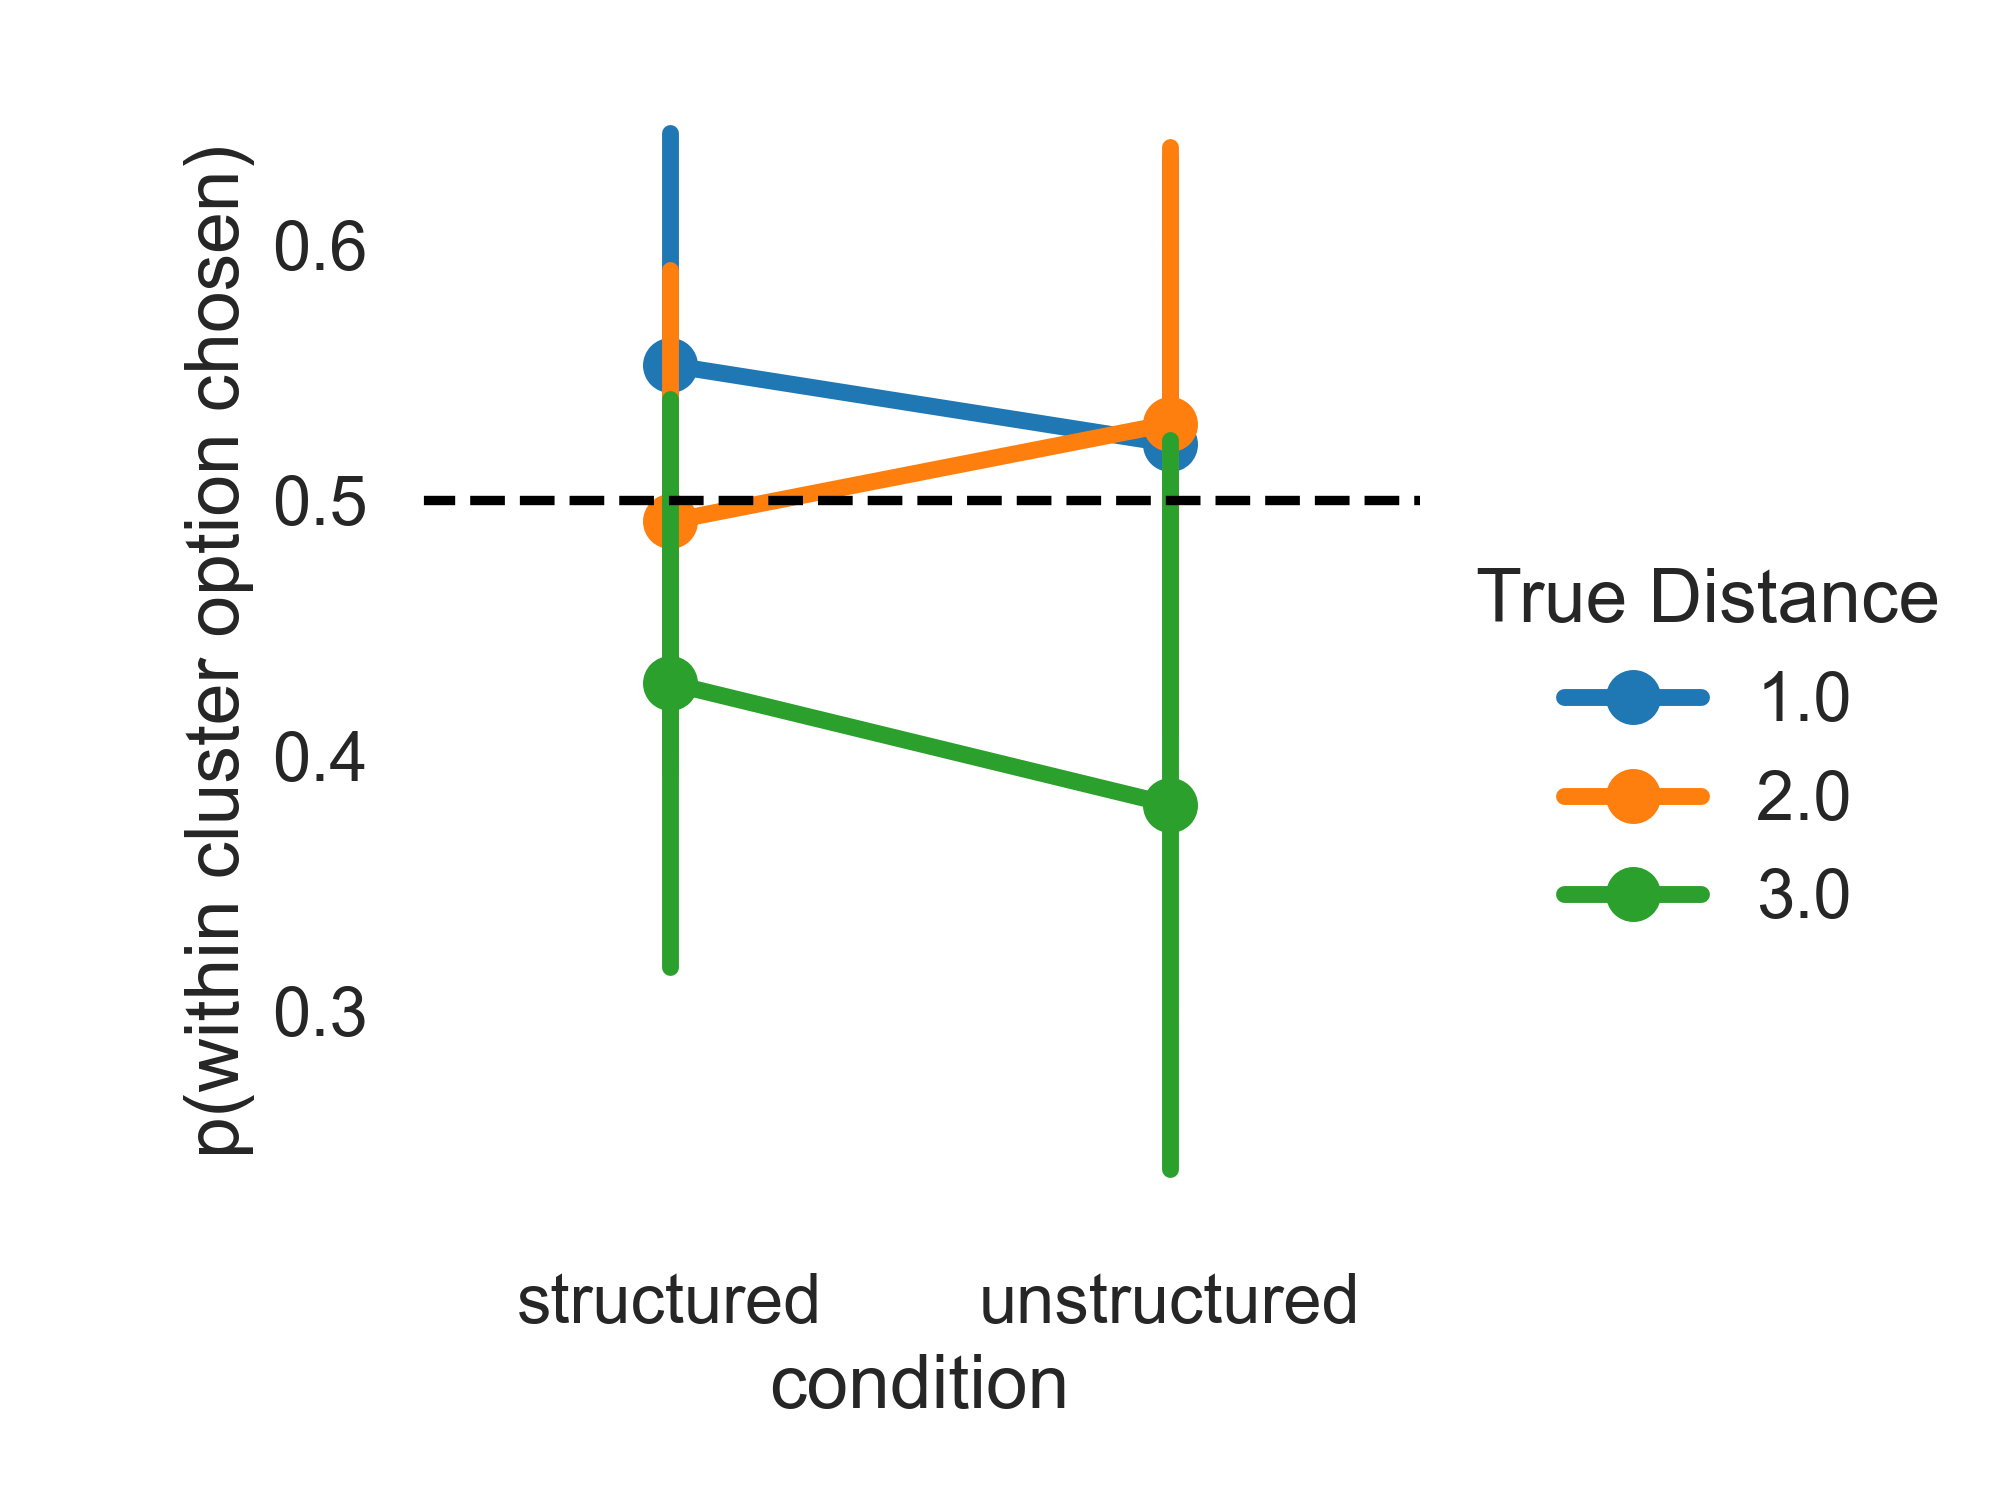
\includegraphics[width = \textwidth]{chapter_notebooks/chapter_3/figures/exp3_choice_results.png}
    \caption{Proportion of trials where the within cluster option was chosen when the distance between and within clusters were equal (ranging from a distance of 1, 2, and 3 connections).}
\end{figure}

\begin{table}
    \centering
    \label{tab:exp3-choice-stats}
    \begin{tabular}{llrr}
        \toprule
         &  & \multicolumn{2}{r}{within chosen} \\
         &  & mean & std \\
        condition & true distance &  &  \\
        \midrule
        \multirow[t]{3}{*}{structured} & 1.0 & 0.565 & 0.497 \\
         & 2.0 & 0.505 & 0.501 \\
         & 3.0 & 0.450 & 0.500 \\
        \cline{1-4}
        \multirow[t]{3}{*}{unstructured} & 1.0 & 0.528 & 0.501 \\
         & 2.0 & 0.533 & 0.501 \\
         & 3.0 & 0.521 & 0.503 \\
        \cline{1-4}
        \bottomrule
    \end{tabular}
     \caption{Proportions of trials where within cluster option at the same distance as the between cluster option was chosen.}   
\end{table}


\subsection{Discussion}

The primary goal of this chapter was to test whether findings in classical explicitly operationalized event boundary literature replicate when boundaries are operationalized implicitly, through temporal statistics. Shared properties between these two boundaries imply shared representations in memory thereby providing a framework for future research to study shared algorithmic processes that lead to formation of event boundaries. 

Under the representation of the SR to acquire boundaries in implicit learning tasks, two predictions were made: (1) Given the three-module graph structure (Figure \ref{fig:modular_graph}), items associated with boundary nodes will be remembered better than items associated with non-boundary nodes. And (2) Given the two-module graph structure (Figure \ref{fig:two_module_graph}), items within the same cluster should be picked at being closer than items across cluster only in a subset of circumstances. Specifically, the model predicts that items at within cluster items distance 1 are the most likely to be being closer and \textit{not} being farther. Furthermore, within cluster items at distance 2 should not be systematically be picked as being closer. Finally, 

The SR-based modeling approach provides a two advantages. First, qualitative pattern in data that matches model predictions provides support for the model and second, qualitative pattern in data that the model does \textit{predict} allows for disproving the model. Thus evidence in favor of the model should incorporate both support for better boundary item member in experiment 3a, and no unexpected distance judgment patterns (for a true distances of 2 and 3) in experiment 3b.

Results of experiments 3a and 3b thus provide support for an SR representation of implicit event boundaries. Furthermore, better memory for boundary items provides evidence in favor of similar representations of implicit boundary events compared to explicit boundary events. On the other hand, however, distance judgment results in this implicit event boundary task do not directly compare with findings from explicit boundary literature. It is possible that lack of an ongoing verbalizable narrative in randomly generated polygons impacts how well neighboring items are bound with each other thereby not allowing us to detect an effect.

DDM is one (highly successful) model of memory that incorporates response time. Other models incorporating response in choice reaction tasks. Several other sequential sampling models can be used in this formulation to provide evidence of better memory strength for boundary items. Most notably, a direct extension of the GCM model for recognition memory is the Exemplar Based Random Walk (EBRW) model \cite{nosofsky2011short}. 

\chapter{Category Learning Through Temporal Abstraction}
\label{chapter-4-category-learning-through-temporal-abstraction}
\section{Introduction}

We naturally categorize items we encounter daily for ease of storage, processing, and decision-making. For example we know instinctively that regardless of shape and form, all lamps form a 'lamp' category based on its function. Several factors determine how we categorize items. Depending on the complexity of rules that determine categories, some categorizations are easier than others \cite{shepard1961learning, nosofsky1994comparing}. Category variability can modulate how often exemplars are classified into that categories \cite{cohen2001category}.

The order of presentation items in category learning tasks has been shown to be an important factor in how category diagnostic features are learned. In particular, when items are presented in a blocked categorical design, participants seem to learn the similarities between the same category items. On the other hand, when items are presented as an interleaved design, participants seem to focus more on learning the features that differentiate the underlying categories \cite{carvalho2017sequence}. As a result of order-dependent differing focus on category diagnostic features, interleaved presentations seem to benefit general category learning. In most prior category-learning tasks assessing order of presentation effects, participants are explicitly asked to learn the underlying categories. There appear to be clear differences when participants focus on learning categories based on how exemplars of these categories are presented \cite{kornell2008learning, kornell2010spacing, whitehead2021transfer, vlach2008spacing, carvalho2014putting, carvalho2017sequence}. In this article, we investigate the effects of order of presentation when category learning is implicit. 

One primary focus on category learning through order of presentation is comparing blocked or interleaved exemplar presentations. For example, \cite{kornell2008learning} showed participants paintings made by two different painters. The order of presentation during exposure was modulated to either be blocked (paintings of one artist shown together followed by the second artist) or interleaved (paintings made by both artists were mixed). When presented with new paintings, and asked which of the two studied artists made them, participants who were exposed to the interleaved format were found to be more accurate at guessing the creator. Category learning also improved for interleaved presentation compared to blocked presentation when tested on items where relevant category features were visually occluded \cite{whitehead2021transfer}. When three-year-old children are tested on the generalization of category-specific features, they appear to benefit from the spaced study of exemplars as compared to a blocked \cite{vlach2008spacing}. By modulating the similarity of presented items, interleaved presentation was found to be better than blocked presentation design on generalization performance particularly when learned exemplars were more visual \cite{kornell2008learning, carvalho2014putting}. 

Interleaved presentation has been theorized to improve in category induction because of context-based variability during encoding \cite{glenberg1979component}. Particularly, for each presented item, an observer will store both the item-specific features along with the context in which the item is encoded. During interleaved presentation, a category diagnostic feature gets encoded under different contexts. Thus, that diagnostic feature will be recalled when tested on novel category items within that context. 

Two theories have been proposed to explain this discriminability-based advantage of interleaving. According to the attention attenuation account, when categories are blocked, participants may think that they have learned the relevant category features after viewing a few items and stop paying attention to additional exemplars of the \cite{kornell2010spacing}. On the other hand, according to the discrimination account, the interleaved presentation allows participants to directly compare the differences between exemplars of different categories that are presented close to each other thereby highlighting these differences \cite{kornell2008learning}. In a direct test \cite{wahlheim2011spacing} found that when participants were shown pairs of exemplars, each belonging to a different category, the interleaving benefit was magnified compared to when they were presented as single items. The authors posit that showing pairs of exemplars would enable participants to carefully study and infer distinctions between category features and hence improve categorization performance .Furthermore, the authors find evidence against the attention attenuation theory by observing that classification performance did not differ as a function of the position in which the exemplar was presented in a stream.

This benefit of interleaved presentation is shown to be modulated by the `level' at which categorization occurs. For example, when \cite{mack2015dynamics} modulated exposure time to individual exemplars along with order of exposure, they found that interleaved presentation was no longer beneficial under short exposure conditions particularly when participants were asked to make a more abstract, `super-ordinate level categorization. On the other hand, when exemplars were presented in a blocked format, a lower, `basic' level categorization was hindered. Thus, category knowledge through order of presentation can be modulated by the level of categorization participants are asked to produce.

It is clear that order of presentation of categories matters during explicit category learning. However, the effect of such order of presentation has not been investigated when category learning is implicit. Indeed recent work shows that participants do acquire category knowledge that when presented implicitly instead of being explicitly asked to learn categories. \cite{unger2022ready} found that assessed on category knowledge, participants appeared to learn category structures without being explicitly instructed to do so. This category knowledge was modulated by the strength of association of the category diagnostic features. \cite{unger2023without} later found that when presented with implicit feature-based categories during a cover task, participants were sensitive towards category diagnostic knowledge. 

More evidence for incidental category learning comes from auditory cognition. \cite{gabay2015incidental} found that participants were sensitive to audio categories learned implicitly as measured by increased reaction times when audio-category-to-response mapping was altered. Incidental category knowledge is further modulated by the sampling category distributions from which exemplars are drawn. \cite{roark2018task} show that probabilistic sampling of exemplars leads to weaker category learning compared to deterministic sampling. Incidental category learning can be further enhanced by task-relevant and disrupted by task-irrelevant feature-to-category mappings \cite{roark2022representational}. Incidental learning may also be disadvantaged compared to supervised intentional learning when categories are non-linearly separable \cite{love2002comparing}.

More incidental category learning has been studied under the `unsupervised' category learning. Participants could infer rules based on correlating features without being explicitly asked to categorize during exposure \cite{billman1996unsupervised}. Category-related items were recognized better when presented close to each other then when category-unrelated items were \cite{medin1994presentation} with people being able to sort stimuli by a single dimension\cite{medin1987family}. Models of categorization have attempted to explore mechanisms of such unsupervised category learning.  SUSTAIN \cite{love2004sustain} seems to explain several of these unsupervised category learning phenomena using a distributed representation whereas ALCOVE \cite{kruschke2020alcove} further provides for error based diagnostic feature attention learning in GCM \cite{nosofsky2011generalized, nosofsky1986attention}.

While implicit category learning appears to be consistent and dependent on several aspects of the underlying categories, unlike explicit category learning, it is unclear whether implicit category learning enjoys the same advantage when category exemplars are presented in an interleaved vs. a blocked design. Most implicit categorization tasks involve manipulation of features as opposed to manipulation of the temporal order of exposure. 

\subsection{Simulating temporal advantage}

Prior work in implicit event boundaries has shown that stimuli shown closer to each other in time develop similar representations in memory and in particular the hippocampus and the medial temporal lobe \cite{schapiro2013neural, turk2019hippocampus, bonner2021object}. Context representations through, for example, SR, can provide algorithmic accounts for such increased similarity between co-occurring events. For example, consider events occurring as the graph in figure \ref{fig:category-graph-structures}

\begin{figure}[ht]
    \centering
    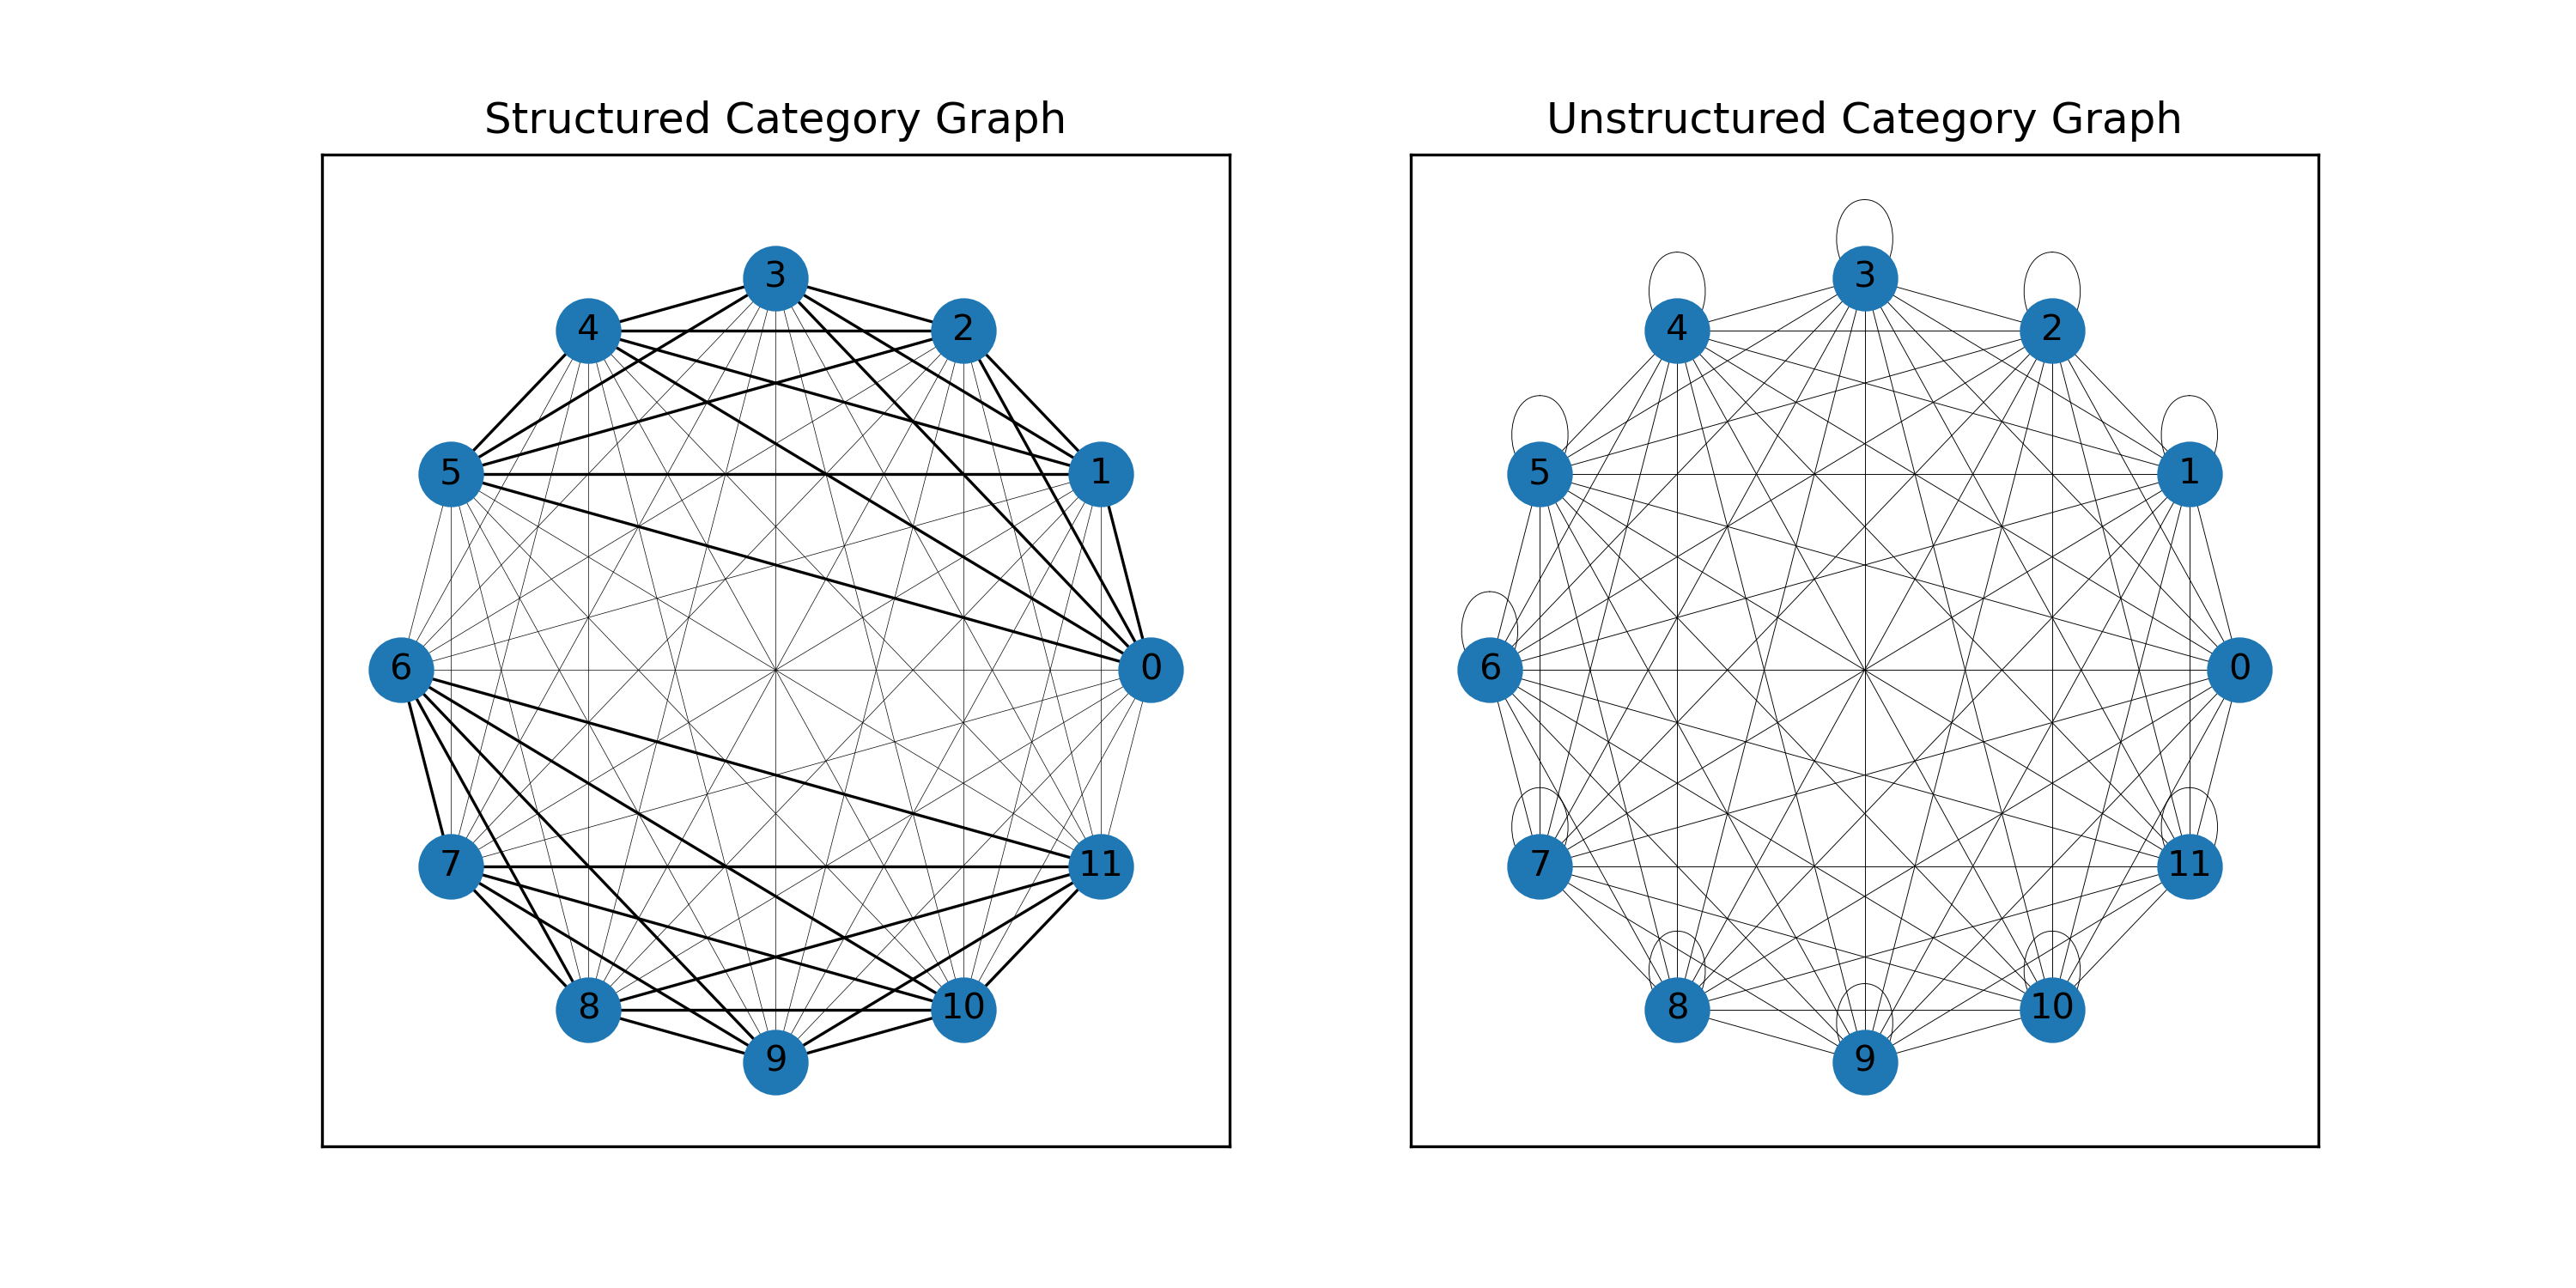
\includegraphics[width = \textwidth]{chapter_notebooks/chapter_4/figures/cat_graphs.png}
    \caption{Graph structures used in categorization experiments. Edge thickness indicates transition probabilities between nodes.}
    \label{fig:category-graph-structures}
\end{figure}

All nodes in both graphs are connected to all other nodes. However, connectivity in the graph on the left is determined by weighted edges -- darker edges are 4 times as likely to be traversed as lighter edges. On the other hand, all edges (including within-node edges) are equivalent in the graph on the right. Since SR represents expected transition probabilities between each pairs of nodes, a (weighted) random walk through such a graph structure produces distinctive representations of context (Figure \ref{fig:category-sr-sims}).

\begin{figure}
    \centering
    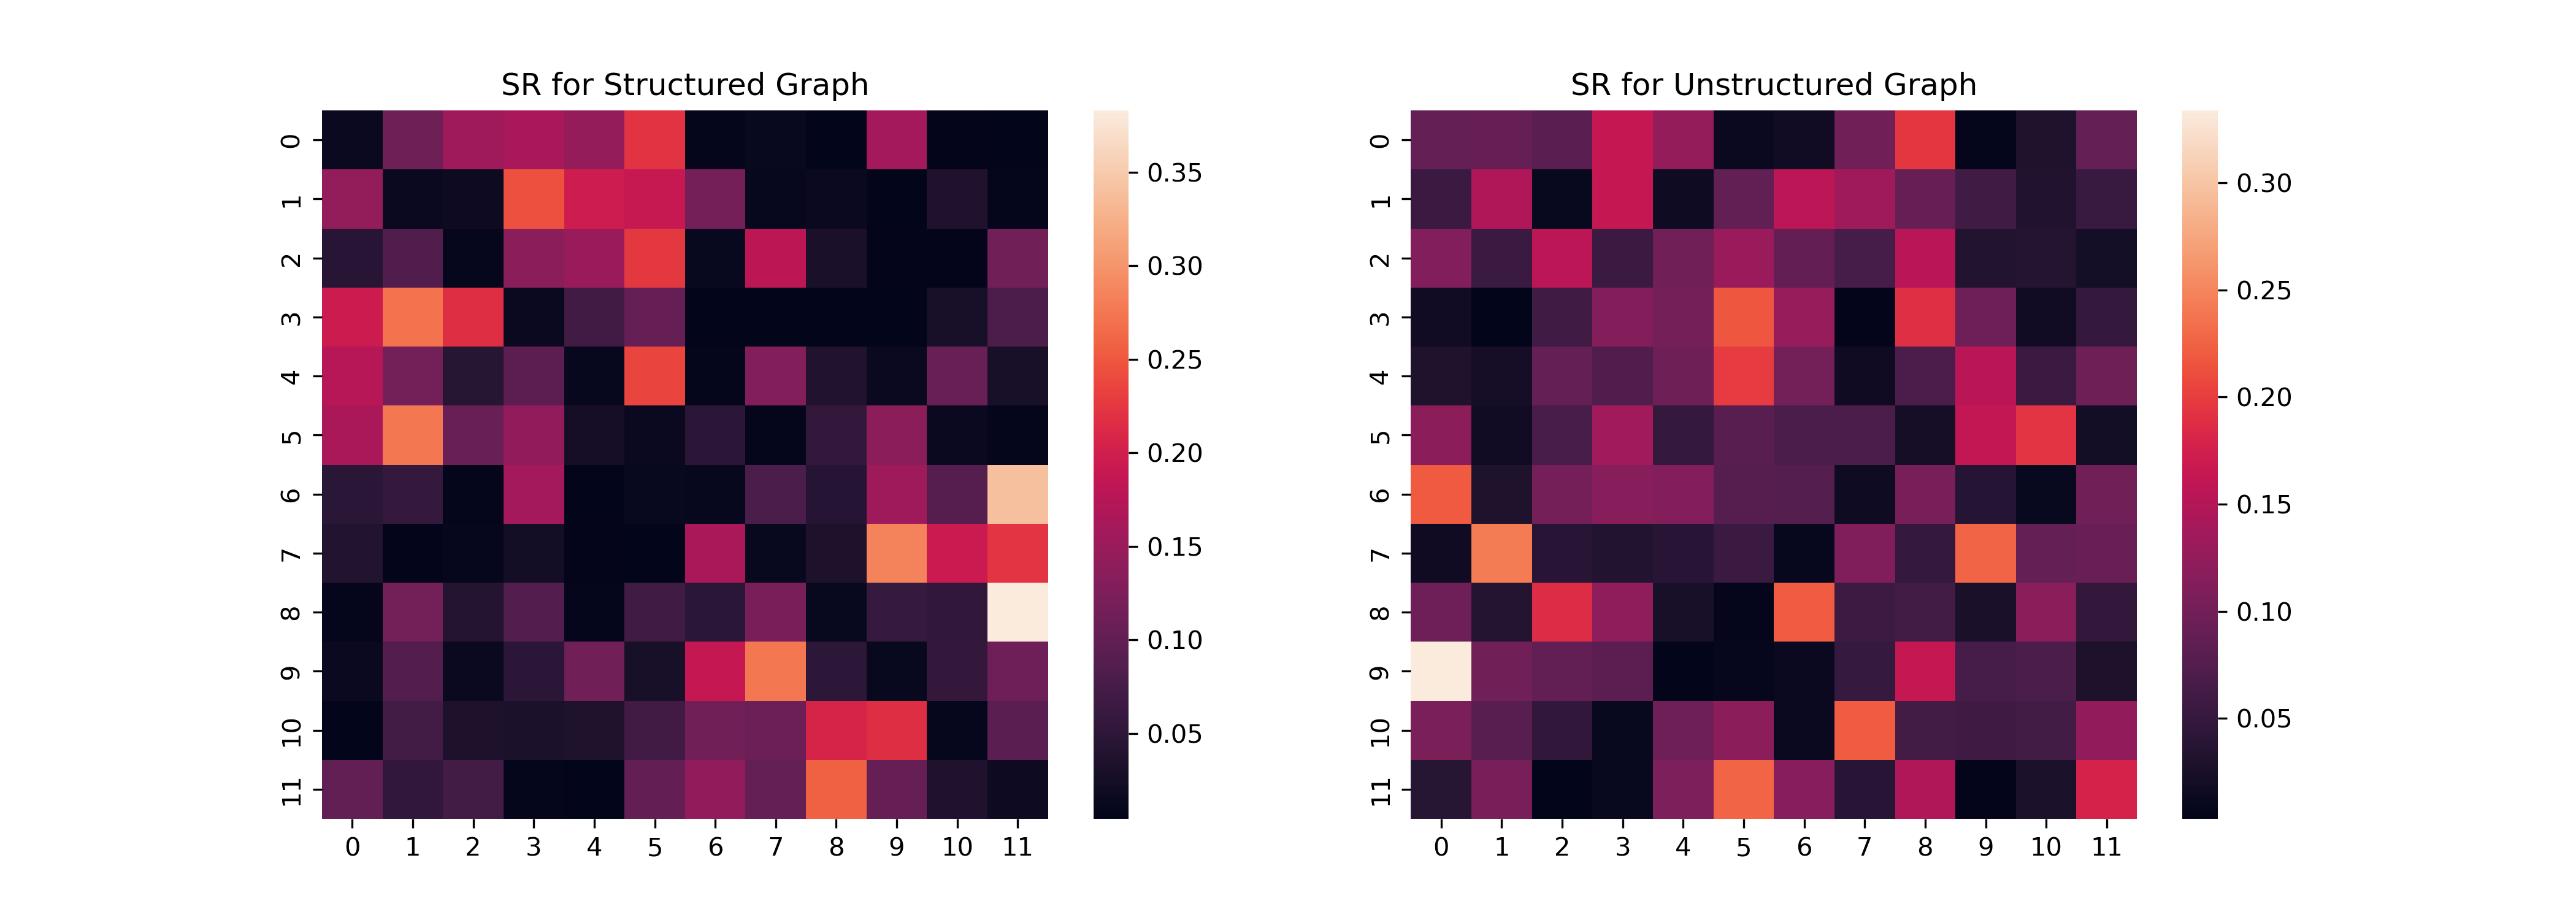
\includegraphics[width = \textwidth]{chapter_notebooks/chapter_4/figures/category-sr-sims.png}
    \caption{SR representations of graph structures used for categorization.}
    \label{fig:category-sr-sims}
\end{figure}

The SR representations thus provides a natural way of representing two temporally defined categories. The key question I ask in this chapter is whether temporal proximity can lead to an increased realization of an inherent visual category structure. That is, in tasks where participants are are unaware of categorization tests or of category diagnosticity of some visual features, does temporal proximity of same-category items lead to a realization of category-diagnosticity of features?

To simulate temporal advantage, I follow the exemplar matching principles from GCM \cite{nosofsky1994comparing,rouder2004comparing,nosofsky2011generalized,nosofsky1986attention}. However, unlike the standard GCM which is used to model categorization learned through explicit feedback of category membership, the tasks presented later in this chapter will not provide any information or an explicit learning signal regarding the true category membership. Additionally, the categorization tests in experiments of this chapter will \textit{not} compare new exemplars with stored category exemplars in memory (especially since no stored exemplars will have an explicit category label). Instead, participants will be asked to compared \textit{studied} exemplars with two new exemplars which maintain most features of the studied exemplars while varying either on a subset of category diagnostic features or category non-diagnostic features. The goal is to thus investigate whether temporal co-occurences cause participants to notice features that are category diagnostic. Finally, unlike traditional GCM, tasks in these experiments use binary valued features to allow for better control of the number of possible feature values and feature dimensions. Few modifications to the formulation of the GCM were therefore necessary. This modified GCM can be formally described as follows:

\begin{equation}
    \begin{aligned}
        d_{ij} = \sum_{m} w_m x_{im} \oplus x_{jm} \\
        s_{ij} = exp(-d_{ij}) \\ 
        p(i|c) = \frac{s_{ic}}{s_{ic} + s_{jc}} 
    \end{aligned}
\end{equation}

where $d_{ij}$ is the bitwise XOR distance between two binary feature vectors representing items $i$ and $j$. $w_m$ is the weighte associated with each of the features. $s_{ij}$ is the similarity between items $i$ and $j$. $p(i|c)$ represents the probability of selecting option $i$ between options $i$ and $j$ given similarities of item $c$ with items $i$ and $j$. Notably, in this formulation of the GCM, the weights of dimensions are only relevant upon mismatch between those features (an assumption in line with other recognition memory and categorization theories such as the Diagnostic Feature Detection Theory \cite{wixted2014signal}).

To incorporate the role of SR-driven context representation, I further assume that the attention weights $w_m$ towards each feature are modulated by SR activations. Specifically, when a stimulus transition is experienced, features that stay constant are facilitated with an increased importance. The magnitude of this increase is assumed to be proportional to the SR representation of the two items. Formally, 

\begin{equation}
    \begin{aligned}
        w_m = \sum_{i, j}^{i_m = j_m} M(i, j)
    \end{aligned}
\end{equation}

Where $M(i, j)$ is the SR activation of item $j$ in item $i$. Feature attentions weights, thus develop over time as items co-occur and the SR matrix $M$ consolidates to represent two clusters seen in figure \ref{fig:category-sr-sims}. This formulation allows to simulate an upper bound of category membership (for a given number of trials and set of parameters). Figure \ref{fig:sr-cat-selection-sims} shows this upper bound for the structured graph where transitions are differentially weighted to create temporal clusters relative to the unstructured graph where all transitions are equally likely. 

\begin{figure}[ht]
    \centering
    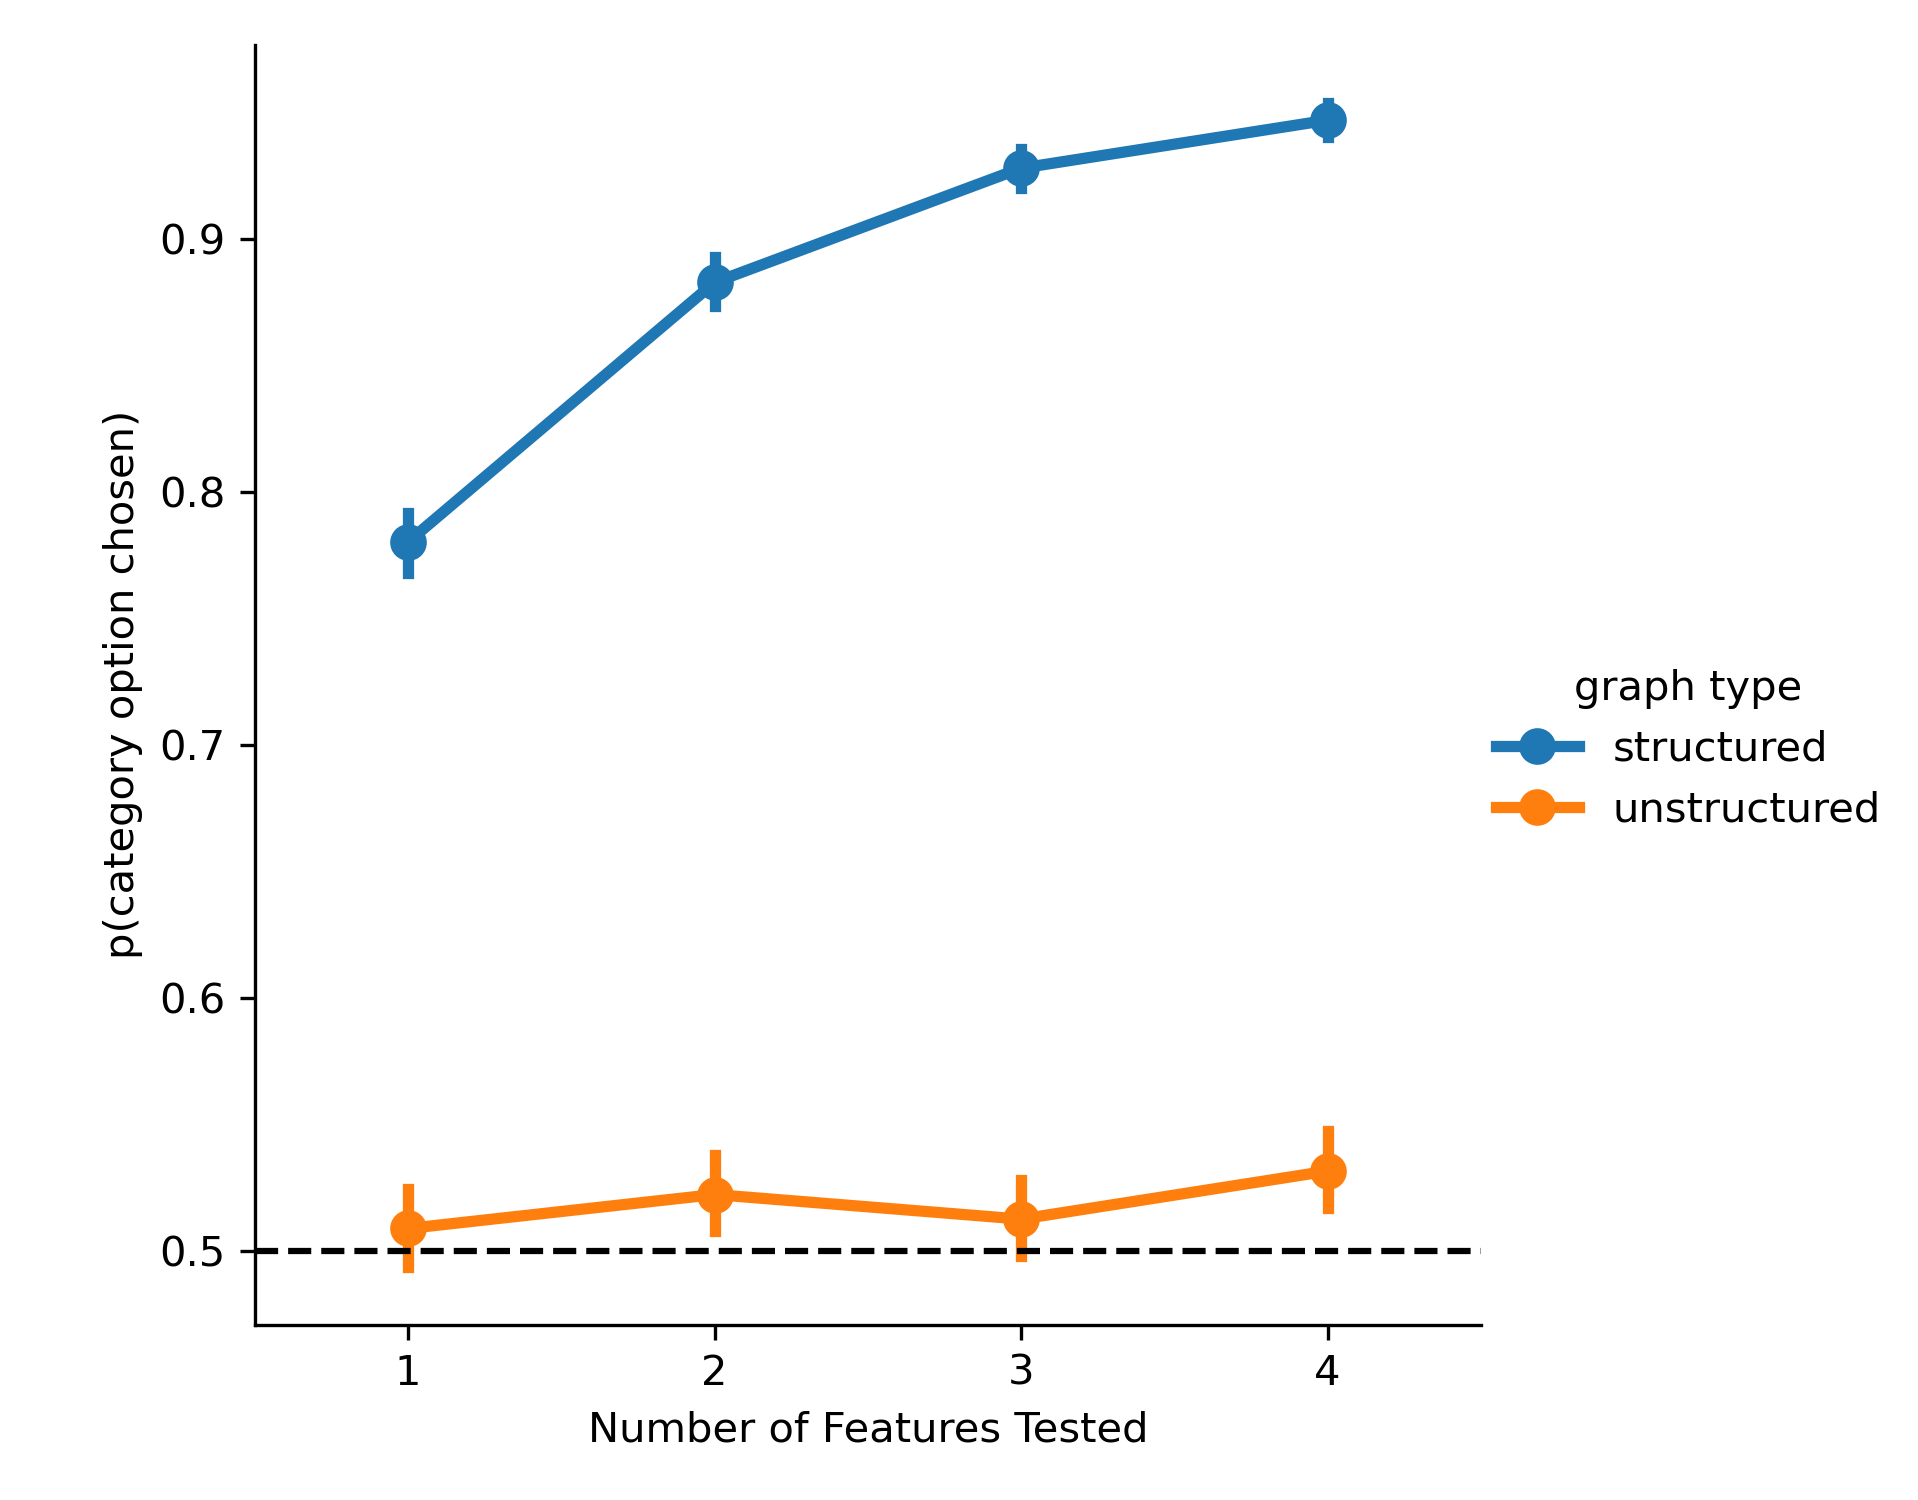
\includegraphics[width = \textwidth]{chapter_notebooks/chapter_4/figures/cat_simulations.png}
    \caption{Simulated proportions of test trials where the option selected will be consistent on its category diagnostic features assuming feature weights modulated by SR.}
    \label{fig:sr-cat-selection-sims}
\end{figure}

In the experiment presented next, I aim to test this model prediction. In particular, participants who are explored to structured graph in binary featured stimuli will consolidate their experience and categorize items based on their (temporally defined) category diagnostic features. Here category diagnostic features are defined by consistency in the values of a feature among aliens that are presented closer to each other. That is, if the probability of going from an alien associated with node 0 to an alien associated to node 1 is high, common features between these aliens are labeled as category diagnostic whereas the features that stay consistent during low probability transitions are labeled as category non-diagnostic features. 

\section{Experiment 3a}

\subsection{Methods}

\subsubsection*{Participants}
58 participants were recruited online via prolific to participate in the study designed in Psychopy \cite{peirce2007psychopy}. Participants were paid \$5 for their time. All study procedures were approved by the University of Massachusetts Institutional Review Board. 

\subsubsection*{Stimuli creation and assignment}
Alien stimuli for used in this study were created using python's Matplotlib library \cite{hunter2007matplotlib}. Each alien consisted of 8 binary valued features, evenly distributed across 4 dimensions (shape, size, color, and orientation). The 8 binary valued features comprised of head color (brown or orange) and torso color (green or purple) for the color dimension; eyes (large or small circles) and arms (large or small lengths) for the size dimension; nose (square or circle) and bellybutton (square or circle) for the shape dimension, and antenna (pointing inwards or outwards) and feet (pointing inwards or outwords) for the orientation dimension. 

One randomly chosen feature from each dimension was chosen as a `category diagnostic' feature whereas the other was deemed as non-diagnostic. Category diagnosticity of a feature was determined based on cluster assignment in figure \ref{fig:category-graph-structures}. Specifically, all category diagnostic features in the same cluster were assigned the same value (for example, all green torsos). In order to equate the number of features of the non-category diagnostic feature, three stimuli in a cluster were assigned the same value of a non-category diagnostic features whereas the other three were assigned a different value (e.g. three orange heads and three brown heads). The table below shows example feature values for the categorization experiment. 

\begin{table}
\centering
\label{tab:category-features-example}
\caption{An example set of stimuli with Antenna Orientation, Eye size, Head Color and Nose shape are category diagnostic based on proximity of occurrence.}
\begin{tabular}{lrrrrrrrr}
    \toprule
    Feature Elements & Antenna & Arms & Bellybutton & Eyes & Feet & Head & Nose & Torso \\
    Stimulus &  &  &  &  &  &  &  &  \\
    \midrule
    1 & 0 & 1 & 0 & 0 & 1 & 0 & 0 & 0 \\
    2 & 0 & 0 & 1 & 0 & 0 & 0 & 0 & 1 \\
    3 & 0 & 0 & 0 & 0 & 1 & 0 & 0 & 1 \\
    4 & 0 & 1 & 1 & 0 & 0 & 0 & 0 & 0 \\
    5 & 0 & 1 & 0 & 0 & 0 & 0 & 0 & 1 \\
    6 & 0 & 0 & 1 & 0 & 1 & 0 & 0 & 0 \\
    7 & 1 & 1 & 0 & 1 & 1 & 1 & 1 & 0 \\
    8 & 1 & 0 & 1 & 1 & 0 & 1 & 1 & 1 \\
    9 & 1 & 0 & 0 & 1 & 1 & 1 & 1 & 1 \\
    10 & 1 & 1 & 1 & 1 & 0 & 1 & 1 & 0 \\
    11 & 1 & 1 & 0 & 1 & 0 & 1 & 1 & 1 \\
    12 & 1 & 0 & 1 & 1 & 1 & 1 & 1 & 0 \\
    \bottomrule
\end{tabular}

\end{table}

This formulation allows to thus test whether temporal proximity of consistent features leads to an increased weights on features that co-occur or whether temporal proximity of the \textit{change} in features (i.e. the non-diagnostic features) leads to increased weights in those features. 

        
\subsubsection*{Design and Procedure}

The experiment consisted of two phases; an exposure phase and a categorization phase. During the exposure phase, participants were shown one of 12 aliens at a time. After a brief period the alien flipped (randomly) left or right. Participants were asked to hit a key to indicate which direction the alien flipped. 

The order of stimulus presentation was controlled by a weighted random walk through the graph structure in figure \ref{fig:category-graph-structures}. 29 participants were presented a stimulus stream following the weighted structured graph (left panel) whereas the other 28 were presented a stimulus stream following the unstructured graph (right panel). For participants experiencing structured weighted random walk, category diagnostic features remained consistent across transitions with 80\% probability and changed with a 20\% probability whereas the category non-diagnostic features changed with an 80\% probability and remained constant with 20\% probability. On the other hand, the participants in unstructured exposure condition experienced an equal probability of change across all features. 

\begin{figure}
    \centering
    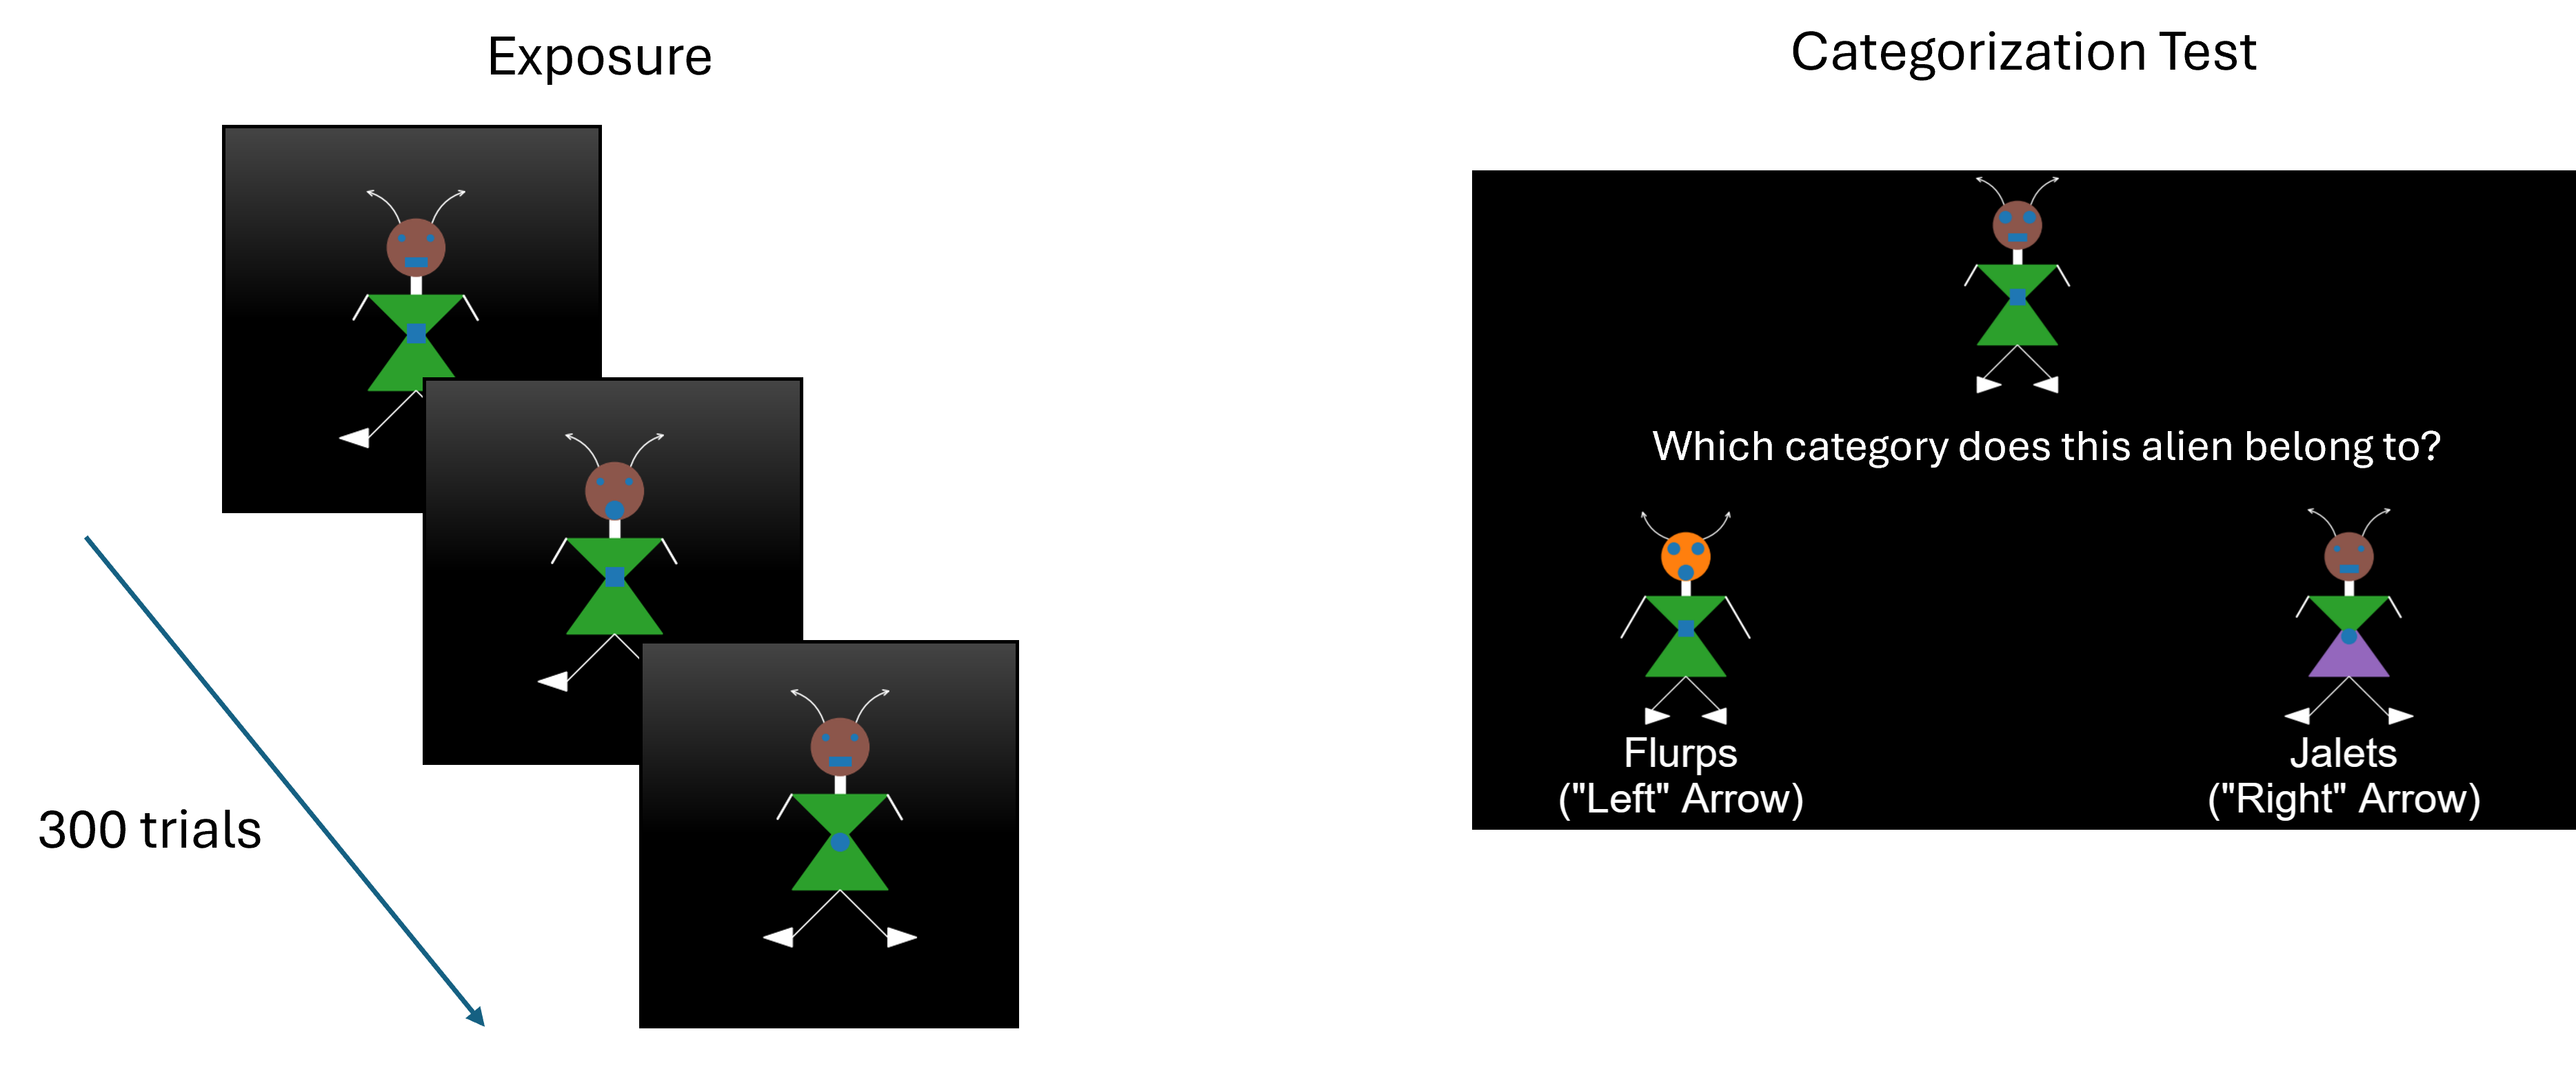
\includegraphics[width = \textwidth]{chapter_notebooks/chapter_4/figures/exp45_design.png}
    \caption{Experiment design schematic for experiments 4a and 4b.}
    \label{fig:exp45-deisgn}
\end{figure}

The general experiment design is shown in figure \ref{fig:exp45-deisgn}. After 300 trials of exposure, participants were asked to categorize the aliens they had seen at exposure. Specifically, for each of the 12 aliens, two options were provided. The category option matched on all category diagnostic features and all but $n$ category non-diagnostic features (where $n in [1,4]$) and the non-category option matched on all category non diagnostic features and all but $n$ category diagnostic features. Participants were asked to select which of the two option does the studied exemplar more relate to in their visual properties. Thus, if a participant selected the category option more often in the structured case, temporal proximity of consistent features increases the weight of shared feature values. On the other hand, if a participant selected the non-category option more often in the structured case, temporal proximity of non-consistent features increases weights of the non-shared feature values.

\subsection{Results}

\begin{figure}[h]
    \centering
    \caption{Proportion of categorization trials where a category diagnostic feature (one which remained more consistent over time) was used to categorize items.}
    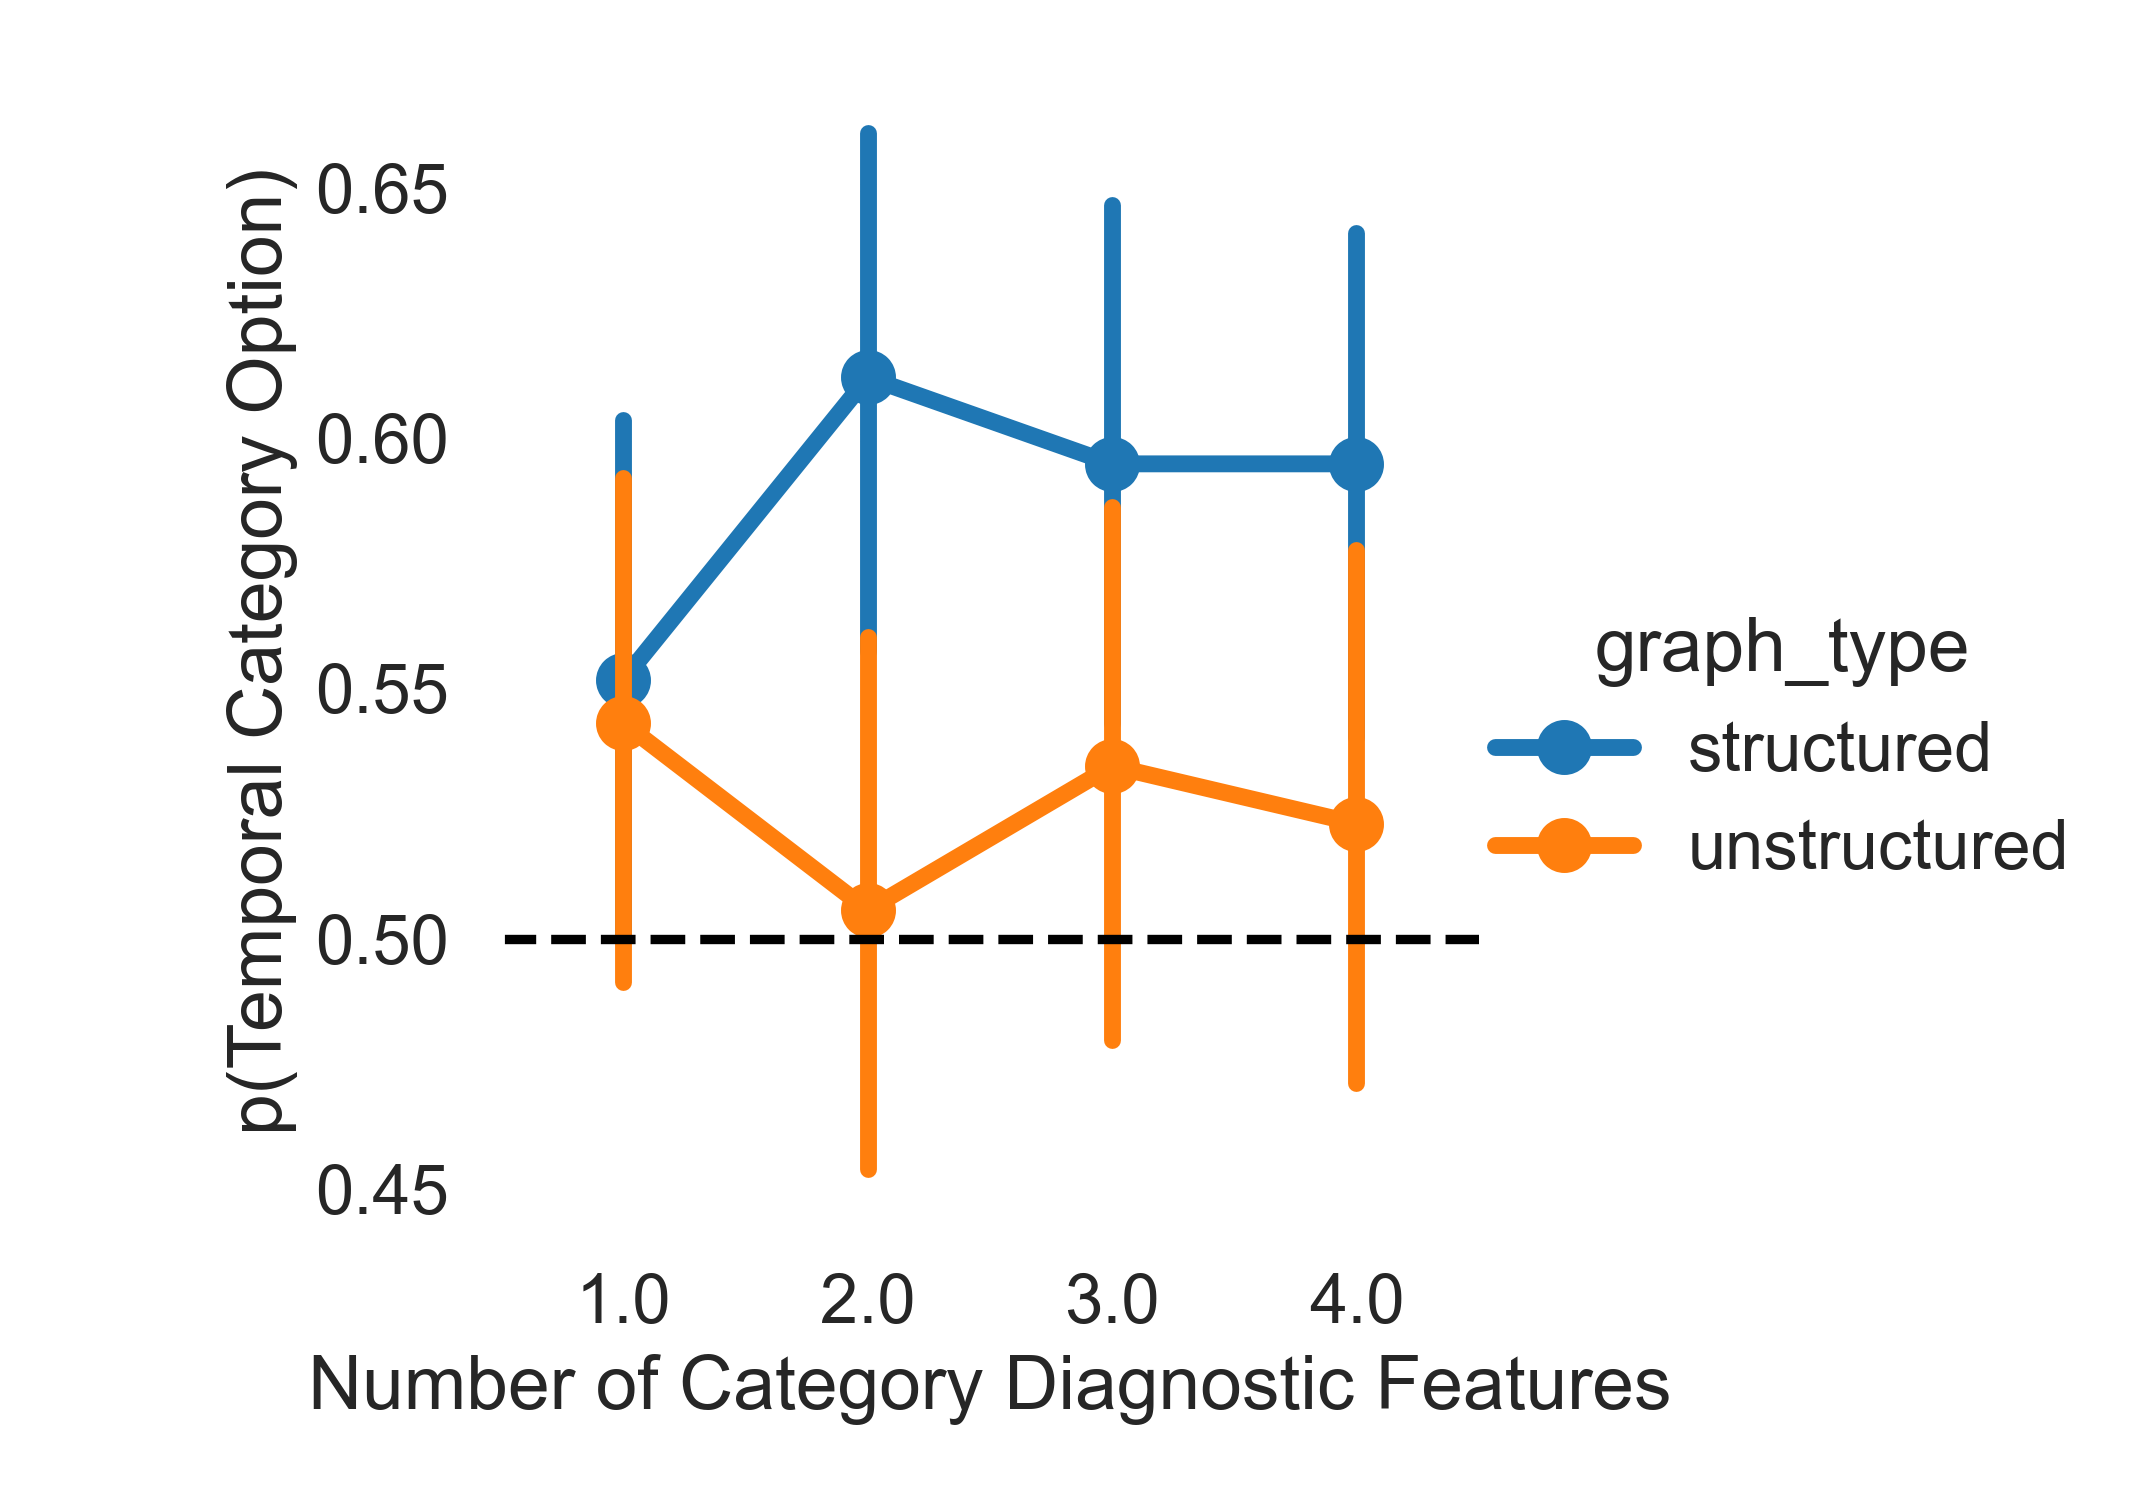
\includegraphics[width = \textwidth]{chapter_notebooks/chapter_4/figures/exp4_proportion_results.png}
    \label{fig:exp4a-choice-accuracy}
\end{figure}
The following bayesian model was used to estimate the effect sizes for categorization based on category diagnostic features for structured weighted walk relative to unstructured walk. 

\begin{equation}
    \begin{aligned}
        1|participant \sim \mathcal{N}(0, Half\mathcal{N}(3.65))
        C(num\_feats):graph\_type \sim \mathcal{N}(0, 7.5)
        \mu = 0  + C(num\_feats):graph\_type + (1|participant)
        p(category\ diagnostic\ option) \sim Bernoulli(\mu) 
    \end{aligned}
\end{equation}

Posterior parameter distributions of chosing the option with common category diagnostic feature in the structured walk relative to unstructured walk are shown in figure \ref{fig:exp4a-bayesmodel-choice-accuracy}
\begin{figure}[h]
    \centering
    \caption{Bayesian estimates of proportions of temporally consistent features used as category diagnostic when exposed to structure relative to when not exposed to structure.}
    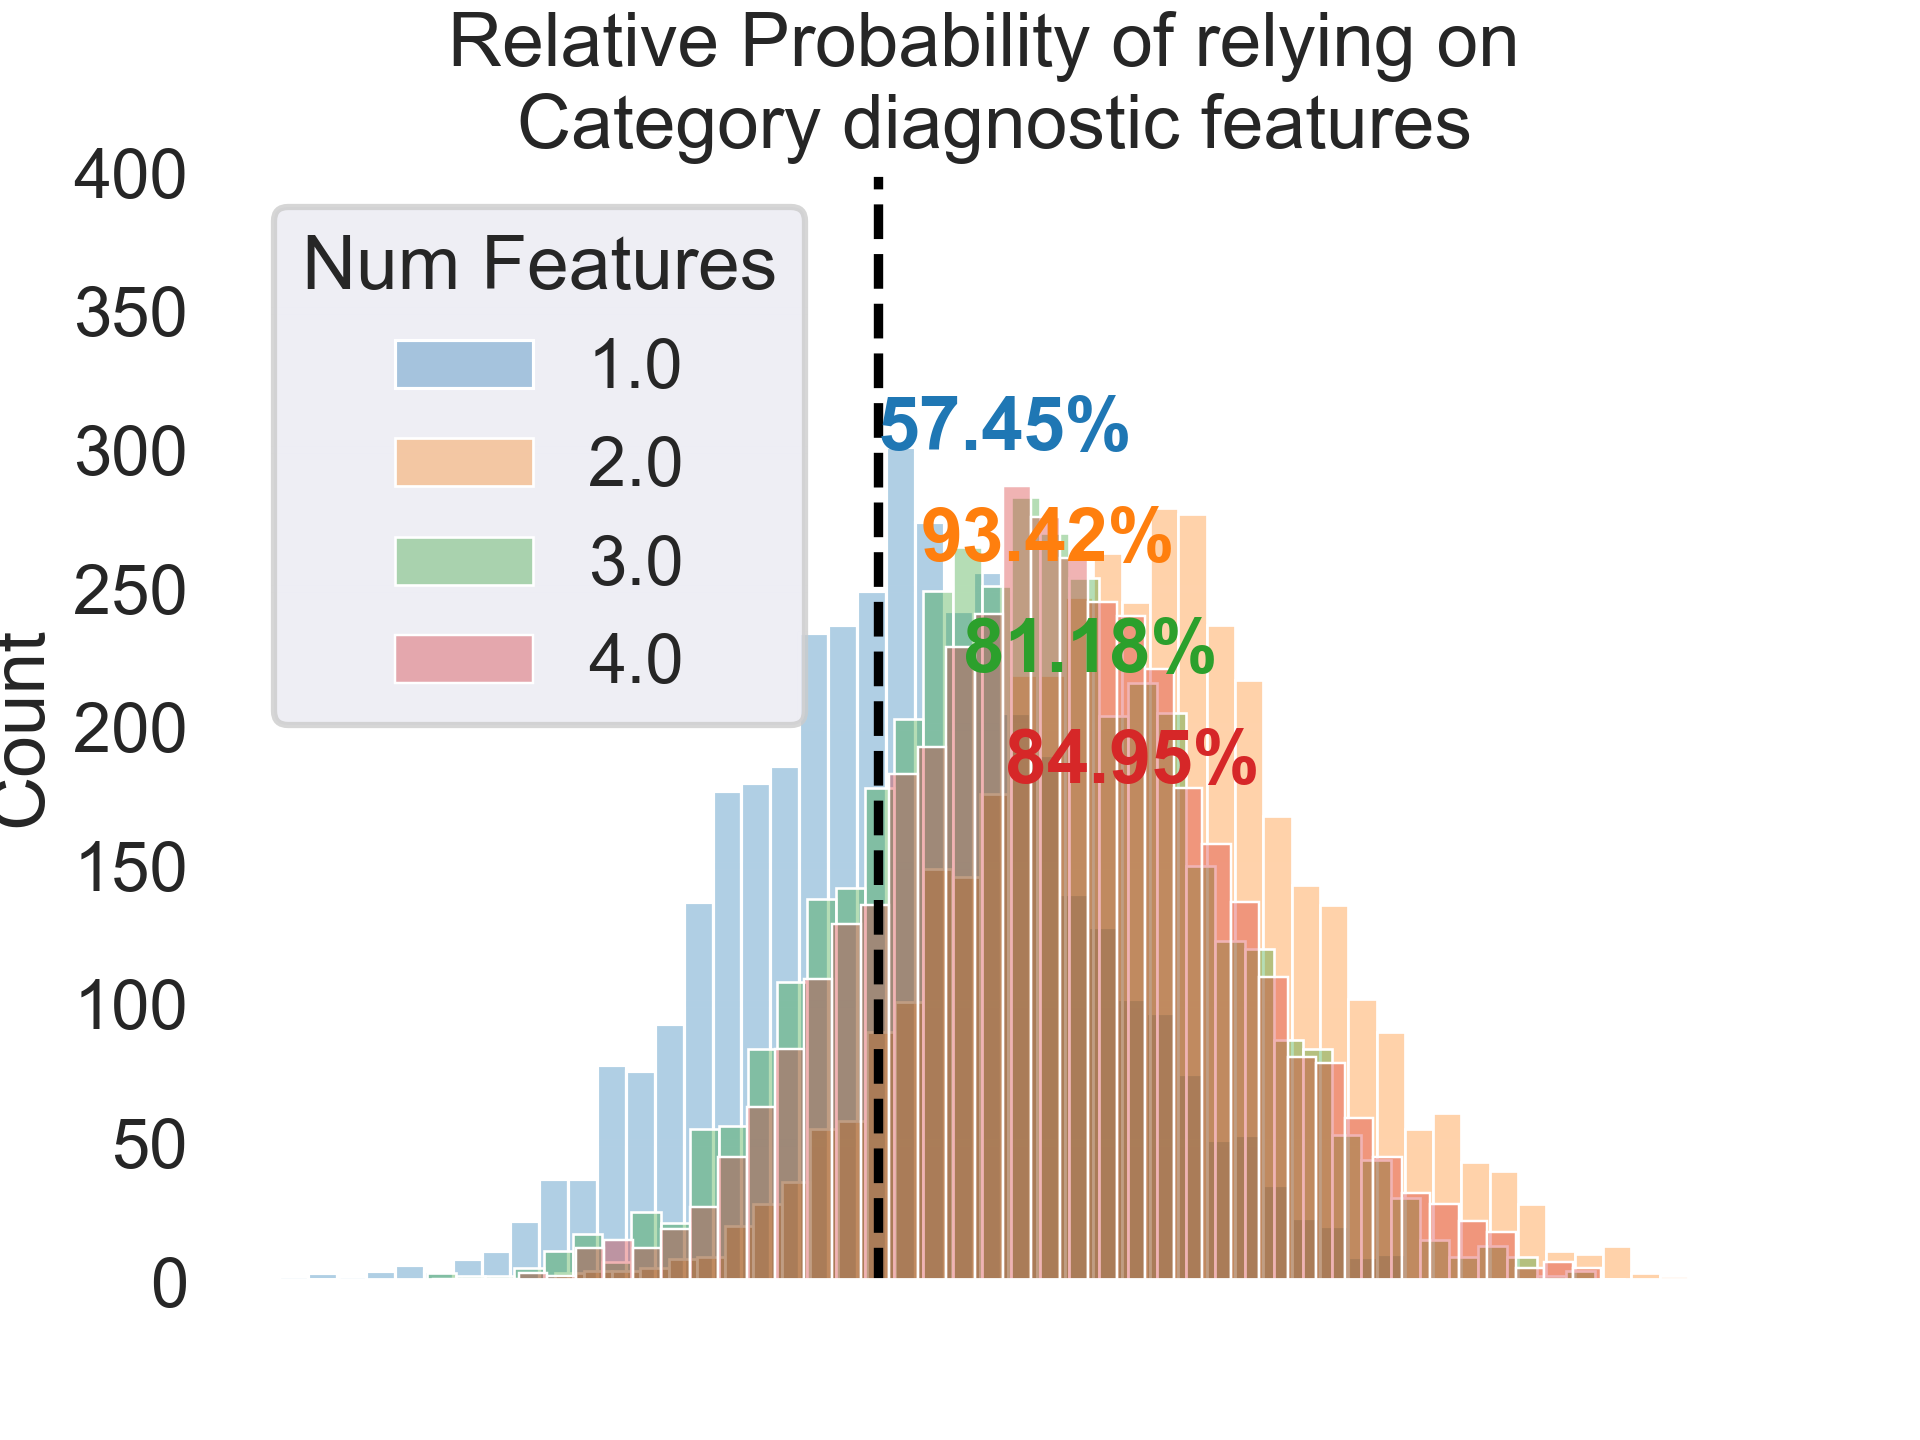
\includegraphics[width = \textwidth]{chapter_notebooks/chapter_4/figures/exp4_bayesmodel_res.png}
    \label{fig:exp4a-bayesmodel-choice-accuracy}
\end{figure}

Results from this experiment thus indicate that participants indeed pick up on features that are consistent between items that are temporally proximal. In the next experiment I aim to extend this finding to assess whether such temporal arrangements can be used as an \textit{intervention} to have participants learn arbitrary features as category diagnostic. Specifically, by using a limited set of features to define a category (as opposed to a pseudo-random selection in experiment 4a). Experiment 4b thus provides (1) An opportunity to replicate findings in experiment 4a, and (2) An assessment whether temporal proximity can be used as an experimental intervention to have participants learn category diagnostic features. 

\section{Experiment 3b}
\subsection{Methods}
\subsubsection*{Participants}
40 participants were recruited over Prolific to complete this 30-minute study. Participants were paid \$5 for their time. All study procedures were approved by the University of Massachusetts Institutional Review Board. 

\subsubsection*{Design and Procedure}
Two groups of participants experienced two different sets of features as category diagnostic. Both groups of participants experienced a weighted random walk during their exposure phase (similar to the structured condition in experiment 4a). For group A, one feature (out of two) for each of the four dimension was chosen to be category diagnostic. For group B, the other feature was category diagnostic. Specifically, head color, eye size, feet orientation, and nose shape were used as category diagnostic features for participants in group A. Torso color, arm length, antenna orientation, and bellybutton shape were used as category diagnostic features for participants in group B. All other experimental procedures were the same as in experiment 4a (see figure \ref{fig:exp45-deisgn}). 

\subsection{Results}
Figure \ref{fig:exp5-category-proportions} shows the proportion of categorization trials where a category diagnostic feature was used to classify the test item. 
\begin{figure}[h]
    \centering
    \caption{Proportion of categorization trials for which category diagnostic features were chosen to determine category membership}
    \label{fig:exp5-category-proportions}
    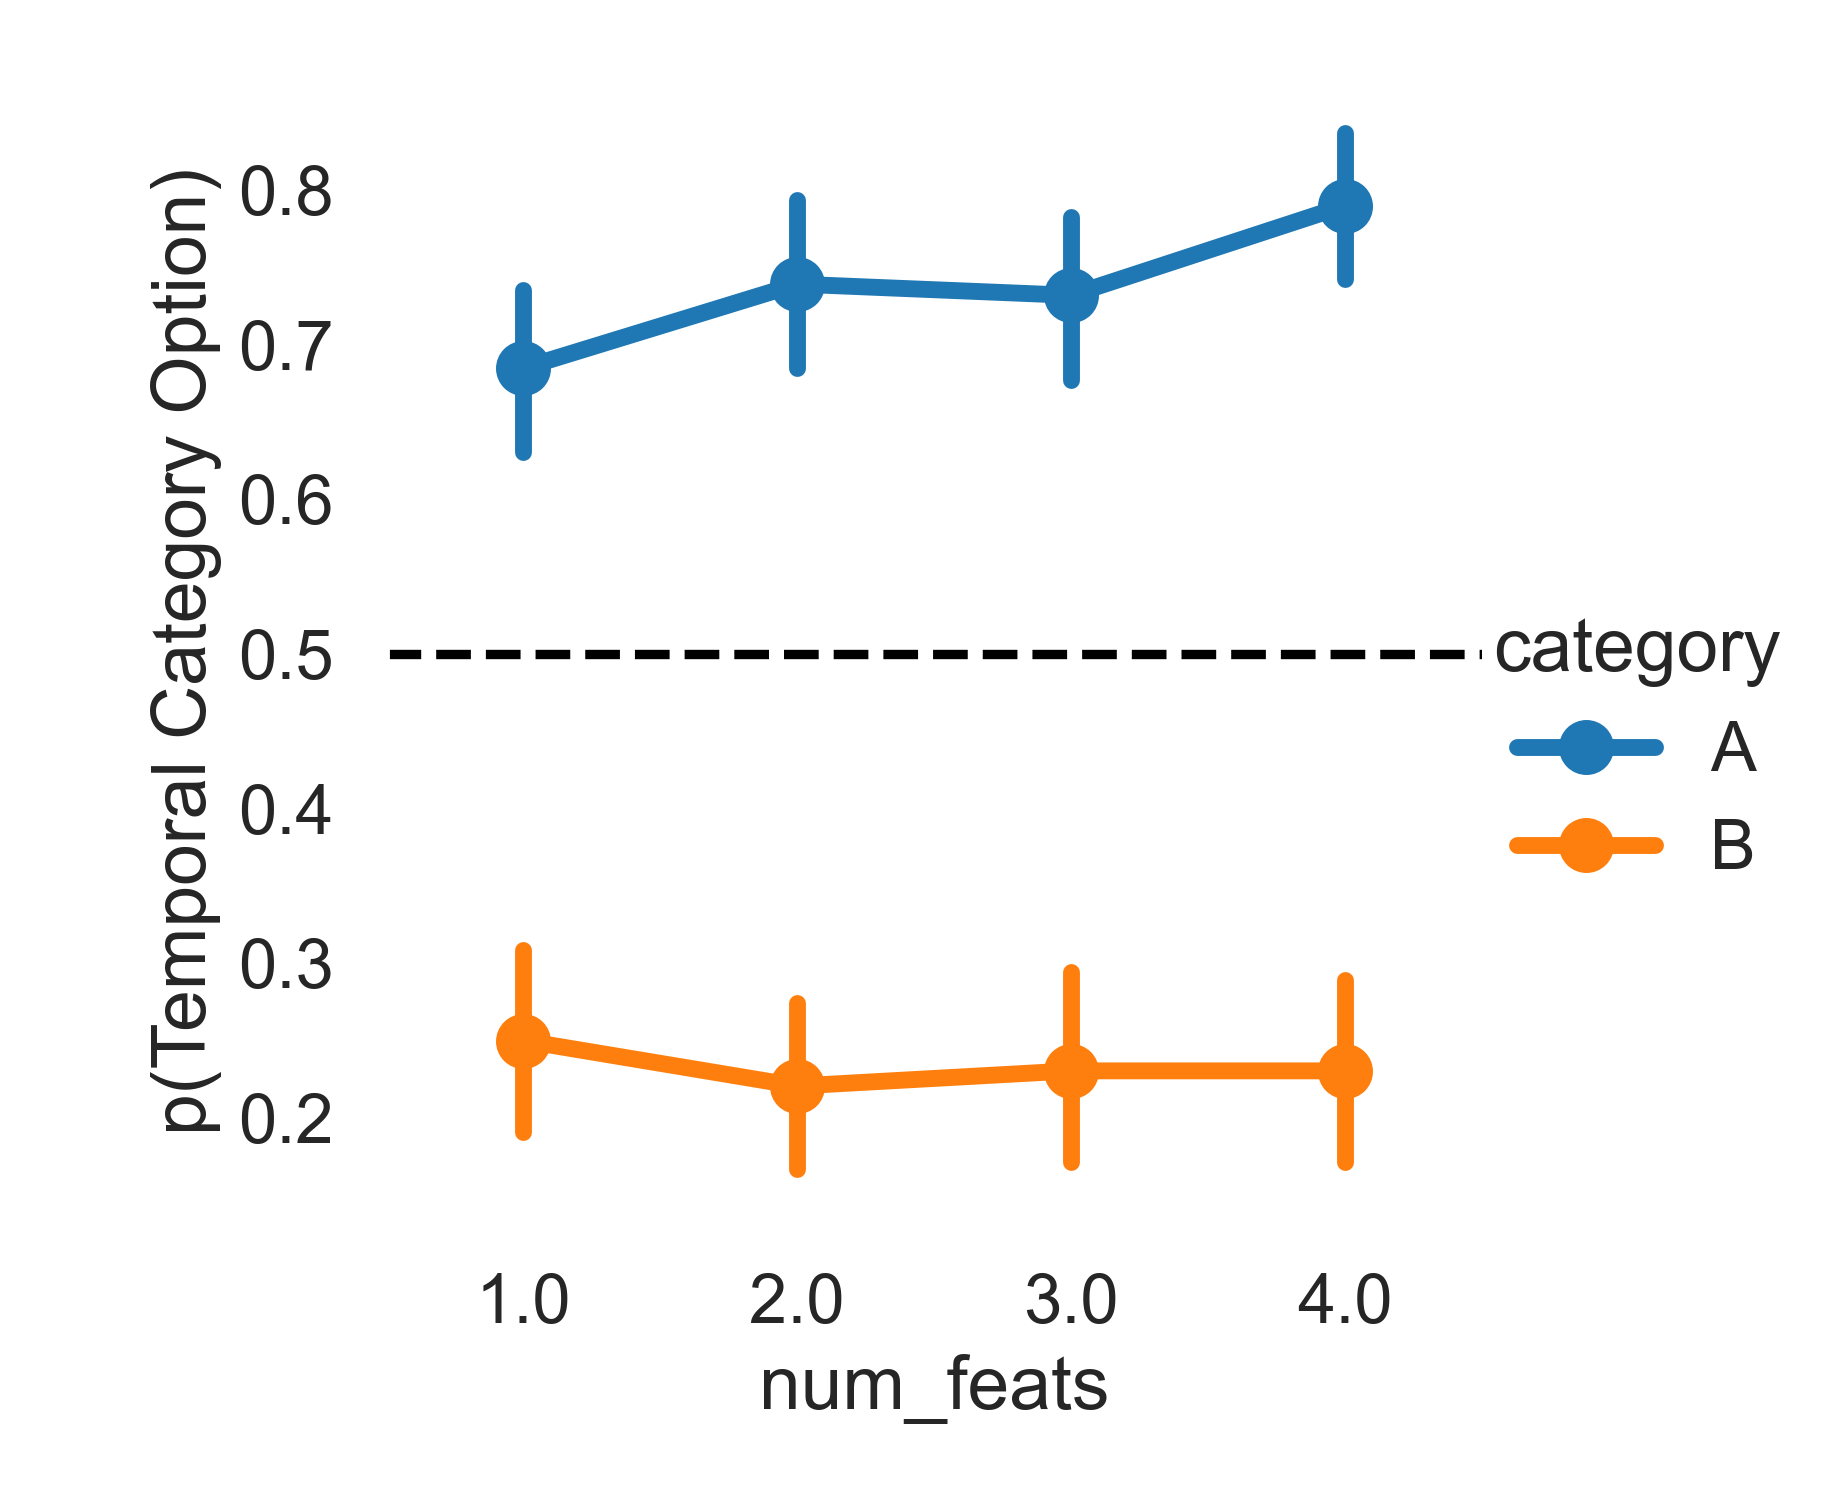
\includegraphics[width = \textwidth]{chapter_notebooks/chapter_4/figures/exp5_proportion_results.png}
\end{figure}
The same model as in experiment 4a was used to estimate effect sizes for both conditions. Figure \ref{fig:exp5-bayesian-estimates-proportions} shows the posterior estimates of these effect sizes. Interestingly, features that were category diagnostic for participants exposed to category A were used to categorize test items. On the other hand, features that were category diagnostic for participants exposed to category B were \textit{not} used; instead category non-diagnostic features (i.e. features that remained consistent during low probability transitions) were instead used to group the test item. 

\begin{figure}[h]
    \centering
    \caption{Bayesian posterior parameter estimates modeling the proportions of temporally consistent features used as category diagnostic for participants exposed to category A (\textit{left panel}) features as category diagnostic and when participants were exposed to category B features as category diagnostic. (\textit{Right panel})}
    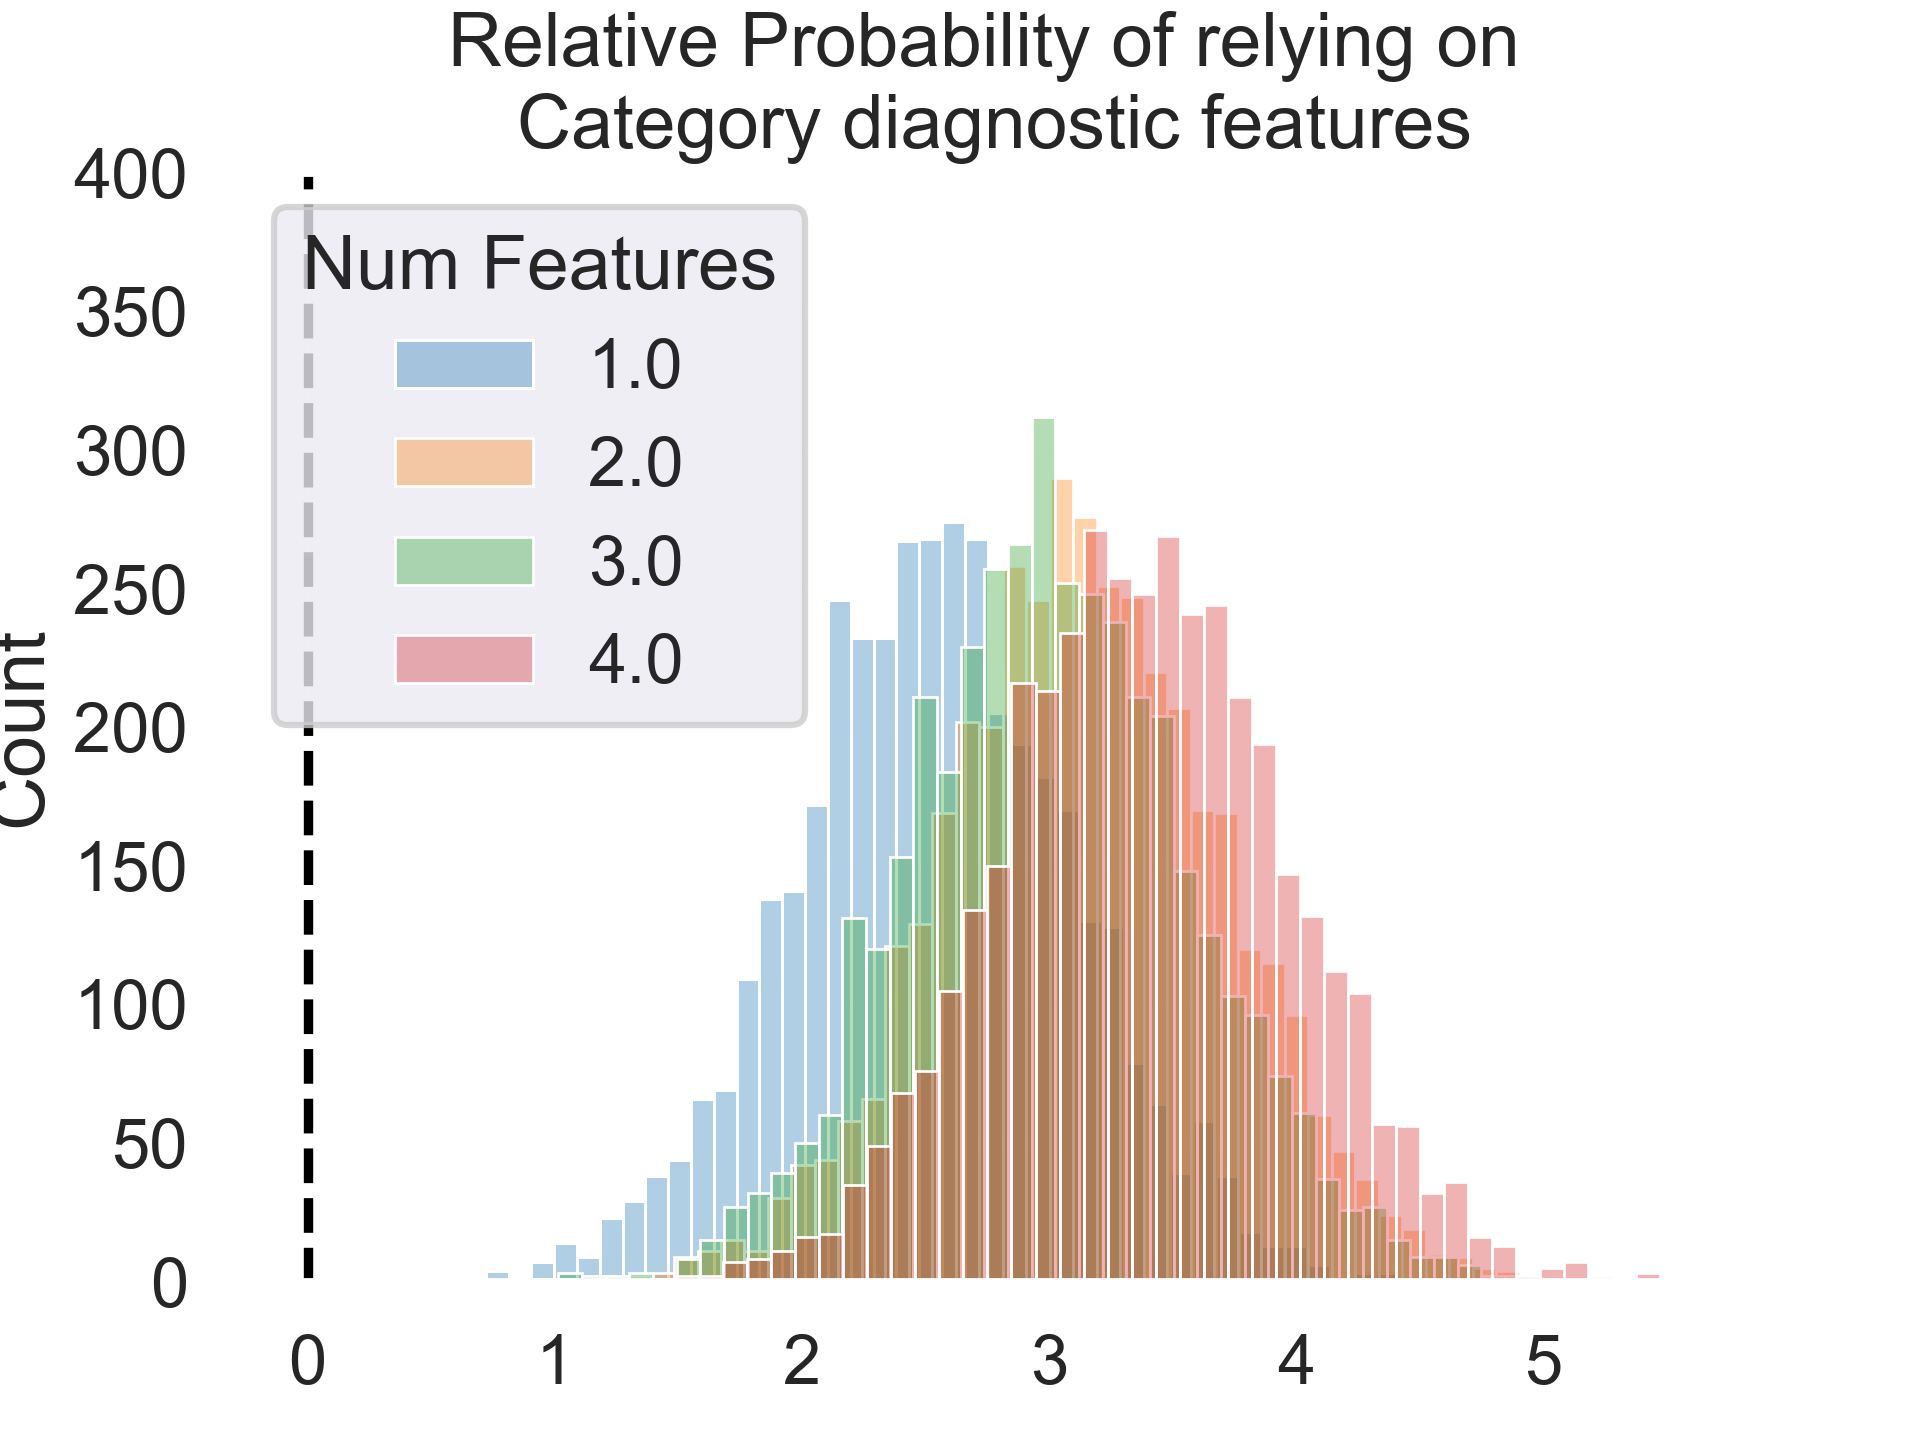
\includegraphics[width = \textwidth]{chapter_notebooks/chapter_4/figures/exp5_bayesmodel_res.png}
    \label{fig:exp5-bayesian-estimates-proportions}
\end{figure}



% In this article, we explore the effects of temporal co-occurrences to manipulate category membership. In particular, we follow the framework of the generalized context model (GCM) \cite{nosofsky1986attention,nosofsky1994comparing, rouder2004comparing}


\section{Discussion} 
The aim of this chapter was to assess if consistency of temporally proximal features leads to category formation. Experiments in this chapter follow a qualitatively similar design relative to past experiments assessing whether category formation is better with blocked design (where items from one category are presented serially after items from another category) compared to interleaved design (where items from all categories are presented together). Unlike past work, the present experiments investigate whether similar (or opposite) benefit exists for tasks where category formation is implicit -- until test, participants were not informed of any categorical structure in the stimuli. 

Past findings in explicit categorization have suggested that category formation is improved with interleaved presentation compared to blocked presentation. However, temporal proximity has been shown to increase representational similarity in the hippocampus \cite{schapiro2013neural}; blocked design may thus lead to realization of consistent patterns based on temporal proximity. Assuming SR as representation for temporal proximity, model simulations show that temporal proximity can indeed lead to categorization. 

Experiment 4a provides support for temporal proximity leading to categorization. However, experiment 4b leads to an interesting update to the model of category learning. When temporal proximity was used as an intervention to category learning, participants picked up on consistency of some features (category A) but on the \textit{differences} of the other features (category B) showing an interleave benefit. 

\subsection*{Model Update}
In the modeling approach shown earlier, two assumptions were made (1) All features were assumed to be equally weighted prior to exposure and (2) Feature weights were modified by consistency temporal proximity -- for each pair of stimuli, if they shared a feature, the weight of the shared feature was proportional to SR representation of the stimuli pairs.  

To incorporate results from experiment 4b, equation 4.2, can thus be modified as follows:

\begin{equation}
    \begin{aligned}
        w_m = w_b * \sum_{i, j}^{i_m == j_m} M(i, j)
    \end{aligned}
\end{equation}
where $w_b$ is the baseline weight for that feature. Updated model simulations are in figure \ref{fig:category-sr-sims-updated}

\begin{figure}
    \centering
    \label{fig:category-sr-sims-updated}
    \caption{Updated model simulations. Base feature weights determine whether more weight is placed on proximally similar \textit{(right panel)} or proximally distinct features \textit{(left panel)}.}
    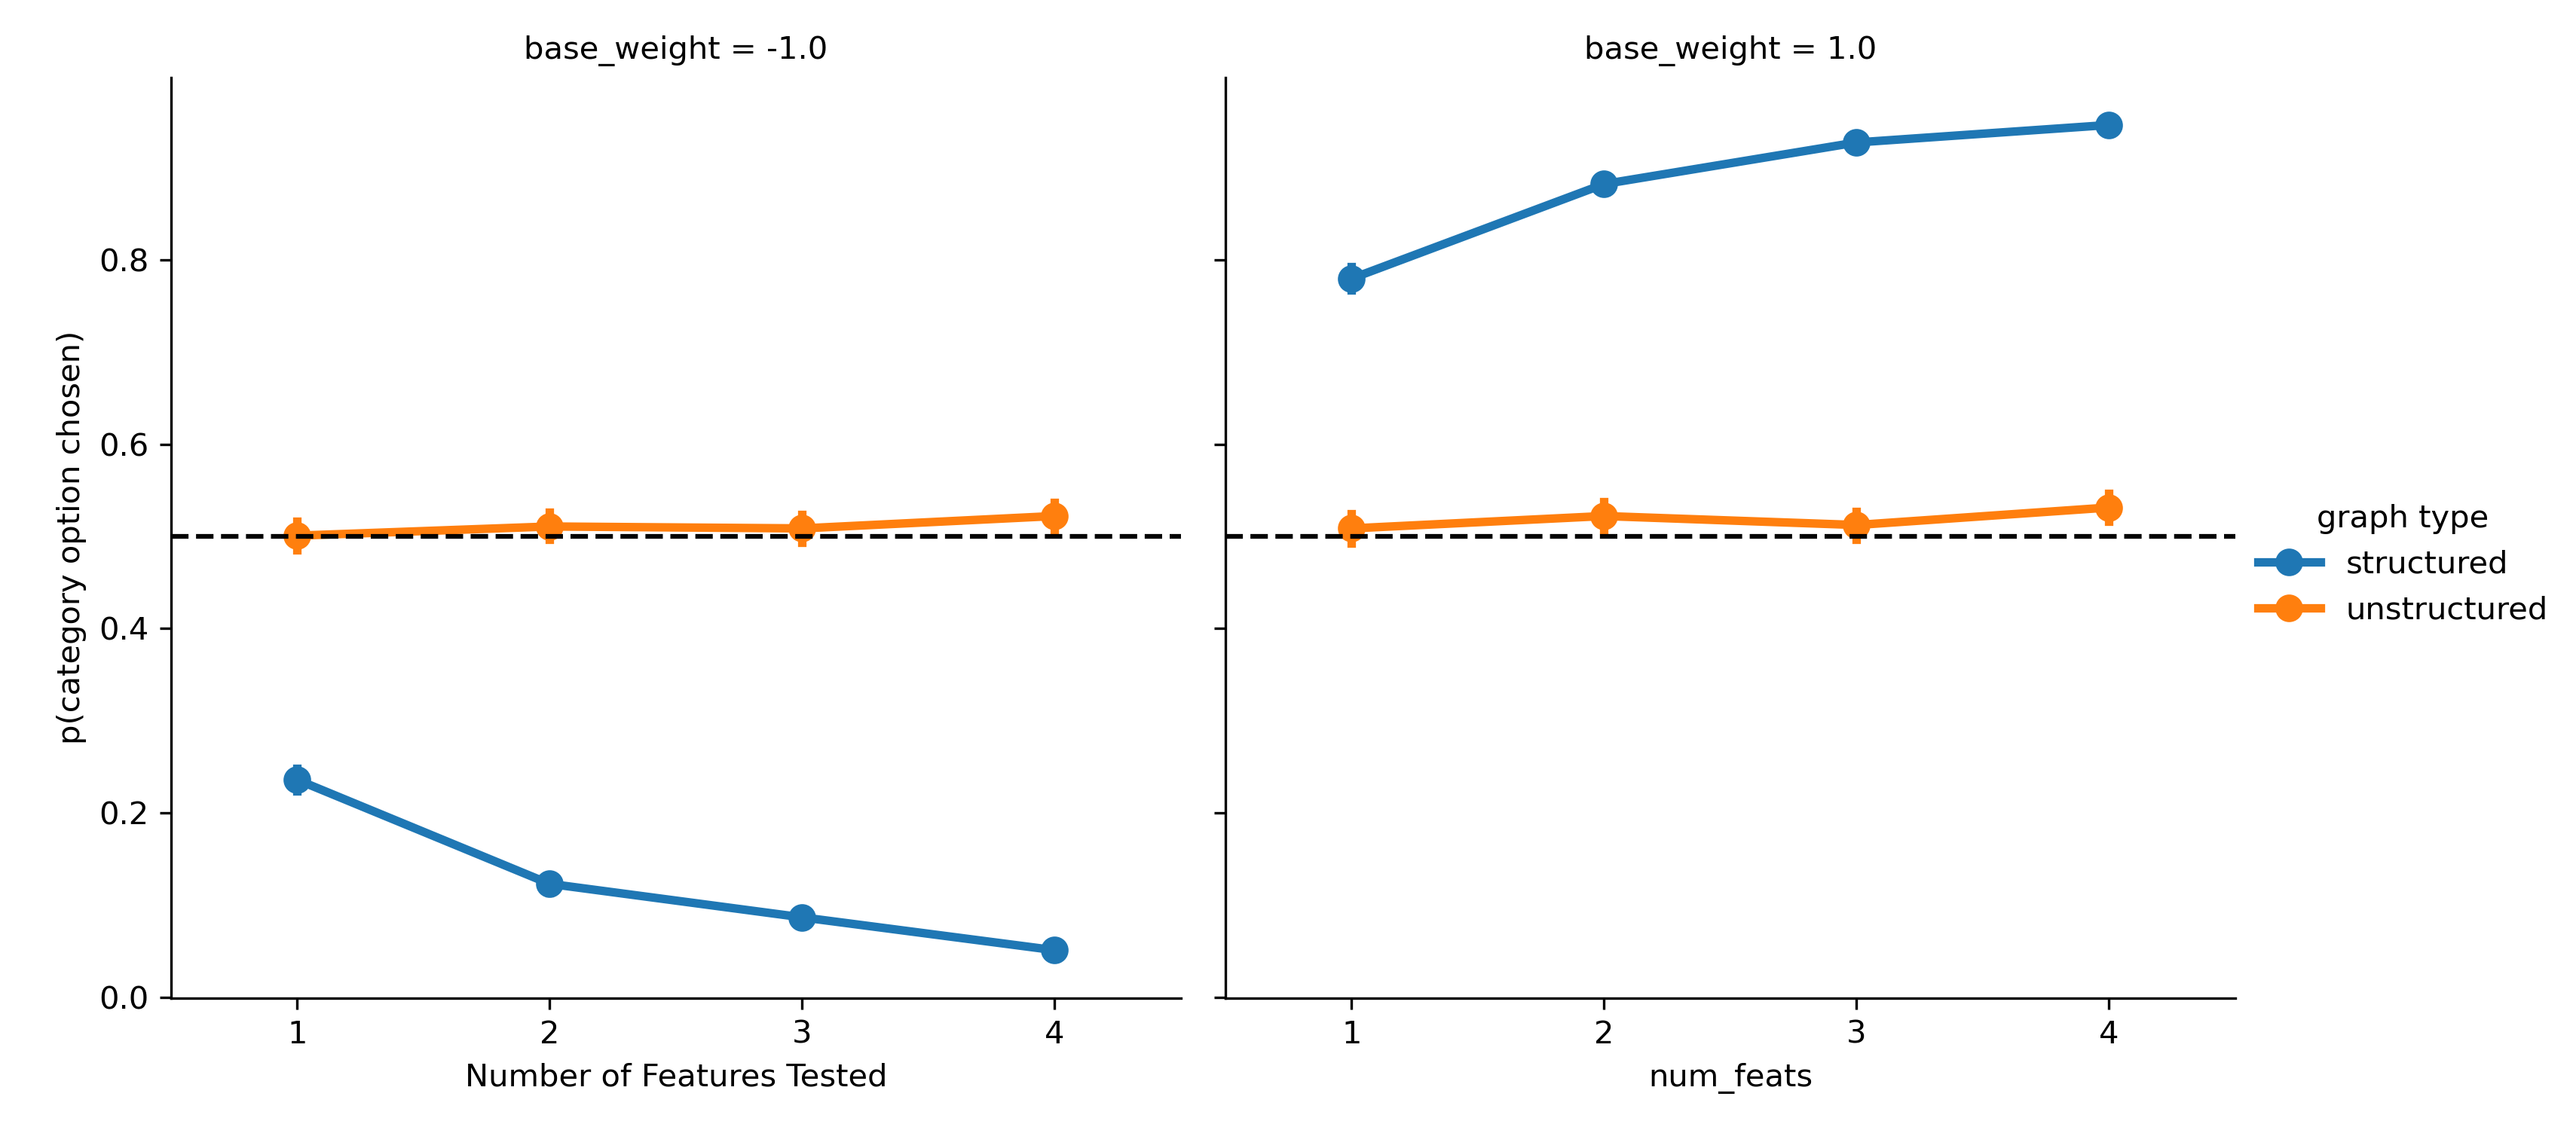
\includegraphics[width = \textwidth]{chapter_notebooks/chapter_4/figures/cat_simulations_baseweights.png}
\end{figure}

The updated model allows for interleaving benefit by increasing the proximally non-consistent feature weights. It is unclear what features lead to an increased attention weight on differences (as would be the case for interleaved categories) or an increased attention weight on consistencies (for blocked categories). Perhaps, features that are more notable lead to an interleaving benefit as more frequent changes in feature values of more notable features become apparent. Norming studies in future experiments can address whether temporal attention benefit depends on baseline noticeability. 

\section{Conclusion}
In this chapter, I demonstrate a use of a context representation framework (specifically predictive representation using SR) to understand the mechanisms behind implicit category learning based on temporal relationships. Findings of these experiments can further model considerations in classical categorization models such as the GCM to incorporate information about temporal presentation order in assigning feature weights. More broadly, given that temporal associations seem to have an effect on how things are visually categorized (albeit, dependent on the specific feature), manipulating temporal associations can be used in more practical settings such as learning natural categories in classrooms. (For example when training students to visually recognize types of geological rocks \cite{nosofsky2018toward, nosofsky2017learning}). 

\chapter{General Discussion and Conclusion}
We experience a stream of continuous information daily. For ease of reference and recall, we break this stream down and store it in meaningful chunks. Event segmentation is a cognitive process that provides mechanisms to break down this temporal stream of information and integrate it across multiple chunks. Prior work has focused on understanding the event cognition process. In the spirit of decomposing cognitive processes into representations and operations on those representations \cite{cowell2019roadmap}, in this dissertation I explore how this process can be assessed through shared representations of temporal structure in memory and operations on these representations. 

In the first chapter, I investigate how representations of ongoing context can produce behavioral patterns in response times. To that end, I contrast two models of context -- the Successor Representation (SR) as a predictive model that maintains context as an expectation of the future and follows error-driven learning with the Temporal Context Model (TCM) as an associative model that maintains representation as current activity and follows Hebbian learning. I show that the two models produce qualitatively different predictions when exposed to varying amounts of limited information about the environment. I then test these predictions in a serial reaction time task and show that data are more consistent with predictions from the SR model.

Prior research and findings in event cognition are often limited to tasks where event boundaries are defined by explicit context changes (e.g. change of scene in a movie). Recently, event boundaries have also been shown to be formed without such explicit context changes but through an underlying temporal structure. However, these implicit event boundary tasks are not typically tested using the same tests used for explicit event boundaries. In the second chapter, across two experiments I assess whether implicitly operationalized boundaries share behavioral properties with explicit event boundaries by (1) Testing whether they are remembered better than non-boundaries and (2) Testing whether events across boundaries are perceived farther than those within. Results from the experiment recognition memory experiment provide support for shared representations between implicit and explicit boundaries. Results from the distance judgment experiment do not provide sufficient evidence for such shared representations. However, combined results from both experiments provide support for SR-based context representations for implicit event boundaries.

In the final chapter, I show that predictive representation of temporal events (such as SR) can be further used to understand the cognitive process of category learning. Prior findings have suggested that there is a differential benefit to presenting different category exemplars in an interleaved fashion vs blocked fashion in category learning. The SR model provides a representational account for this temporal order of presentation effects by modulating attention towards category diagnostic features. While the precise nature of this modulation operation further depends on the specific visual features that define categories, implicit visual category learning tasks in this chapter show, as predicted by SR, that the temporal order of presentation of category exemplars indeed matters in how categories are learned.

It has been argued that boundaries separating events temporally and spatially share representations. This dissertation further advocates for shared (algorithmic) representations across different processes in cognitive psychology. I show that a common predictive representation framework can be useful in understanding and relating implicit statistical and motor learning (chapter 1), event cognition and memory (chapter 2), and categorization (chapter 3). Using a common representation can provide an important algorithmic constraint in understanding different cognitive processes. Future work in cognitive psychology can therefore focus on testing operations on these common representations that may account for observed behavior.

\appendix
\chapter{Chapter 2}

\section{Comparing first and the last blocks}

Similar to comparisons done in the main text, the response times between the boundary and non boundary nodes for the first and last blocks were compared when transitions leading into those nodes were within cluster (i.e. from another non-boundary nodes).

\begin{figure}[H]
    \centering
    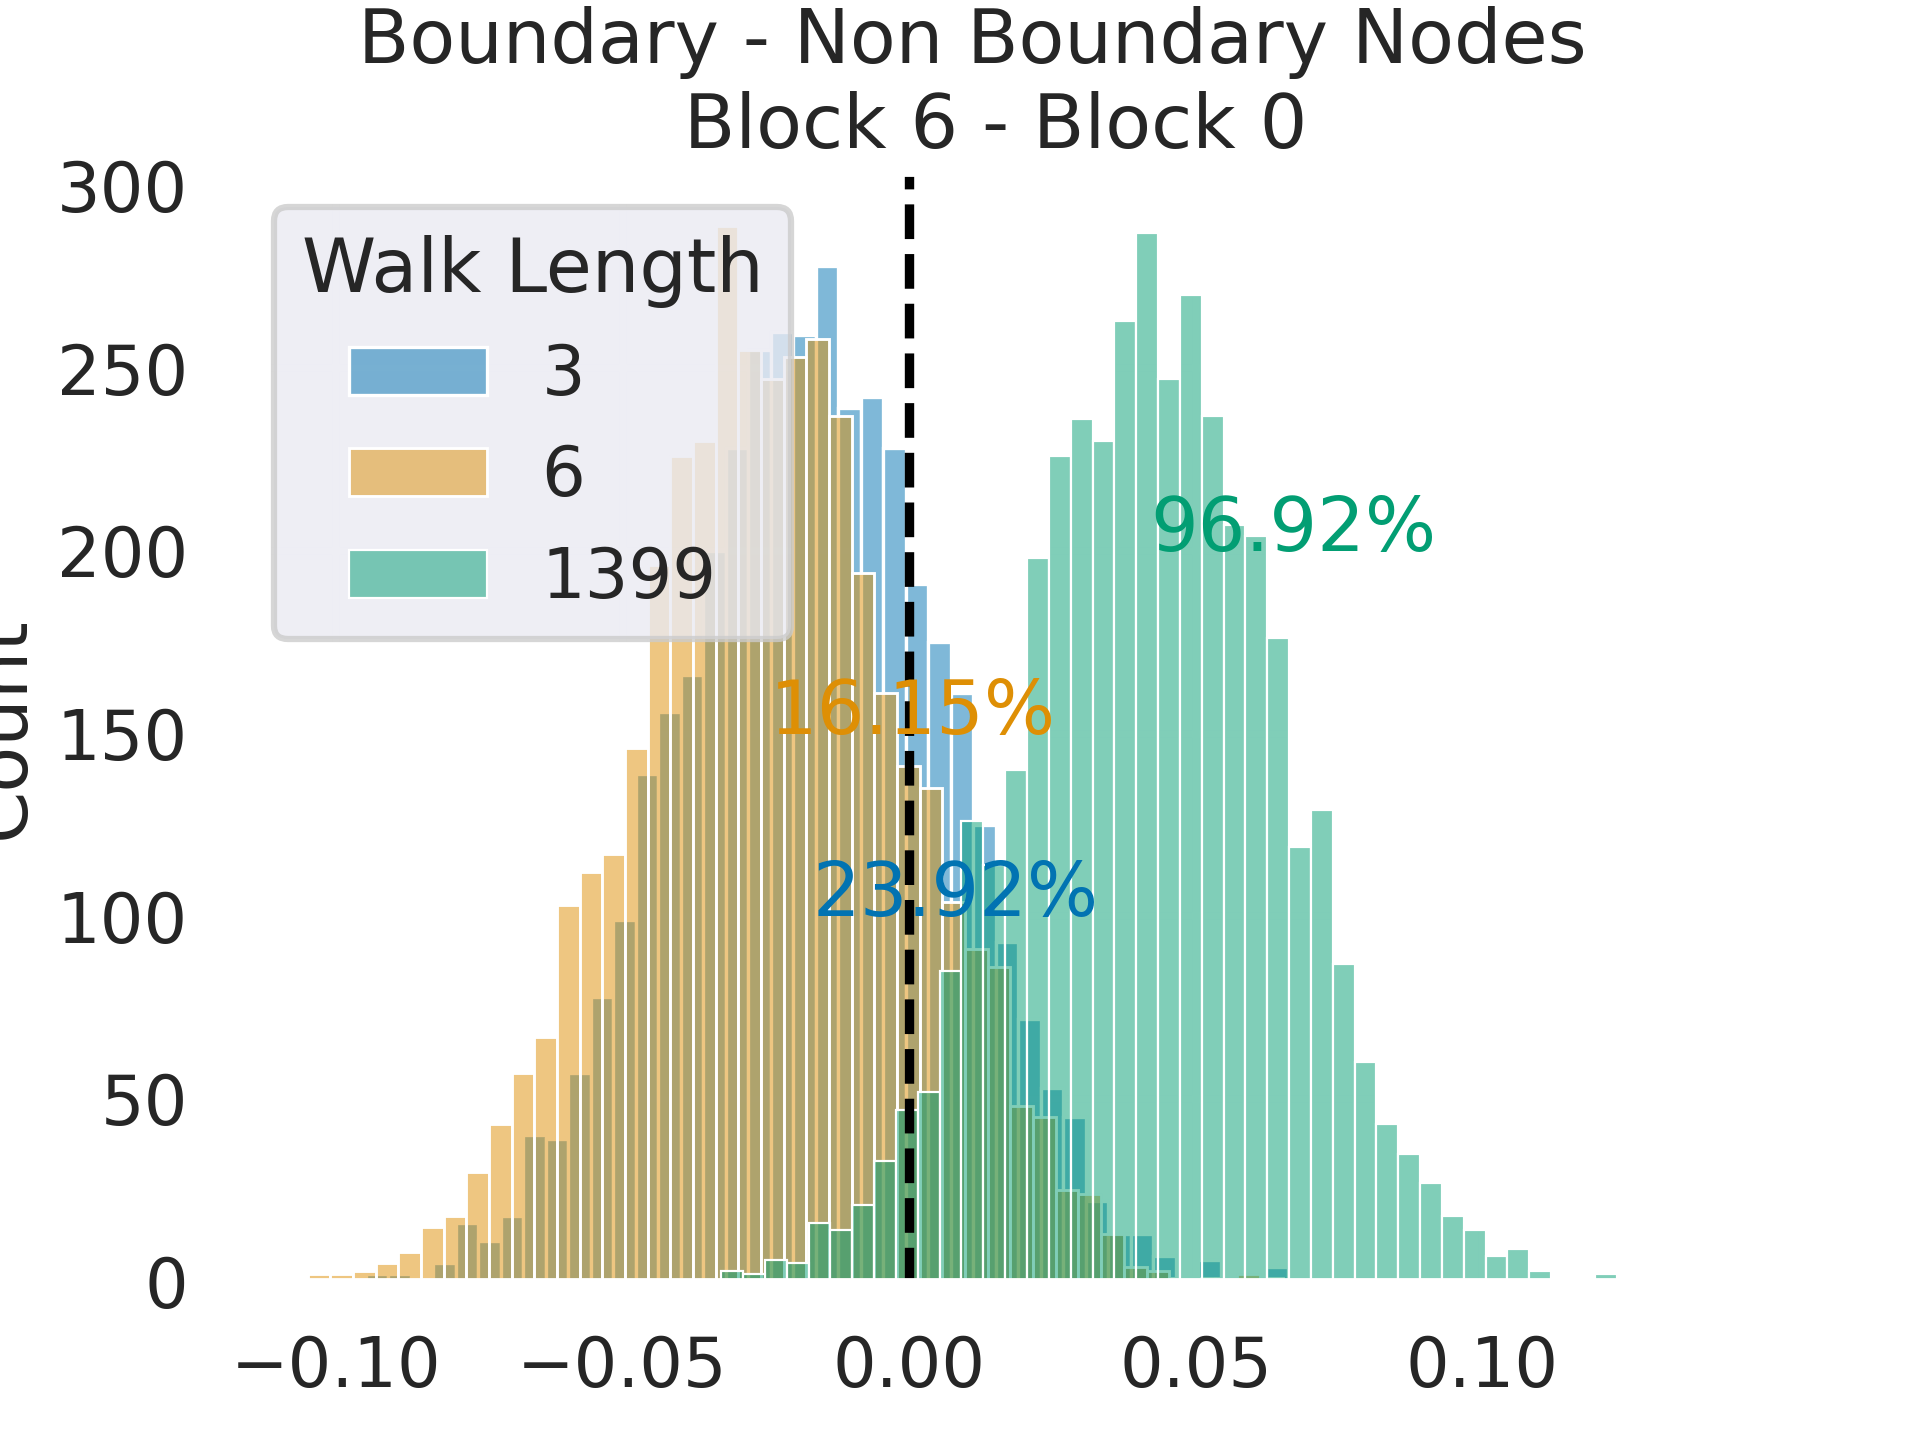
\includegraphics[width = 0.75\textwidth]{chapter_notebooks/chapter_2/figures/nb_b_diff_block60.png}
    \caption{Posterior estimates of comparisons the slowed down reaction times for boundary nodes relative to non boundary nodes. Reaction times slowed down more with larger walk lengths.}
    \label{fig:bayesmodel-firstlastblocks}
\end{figure}

Figure \ref{fig:bayesmodel-firstlastblocks} provides further evidence in support of the SR model. Reaction times decrease across the board. The decrease is lower for boundary nodes than non boundary nodes and this difference increases with walk length providing support for the SR model. 

\section{Fitting the entire learning curve}
The entire learning curve was fit using a linear model to estimate differences in decreased response times between boundary and non boundary nodes over time. 

\begin{figure}[H]
    \centering
    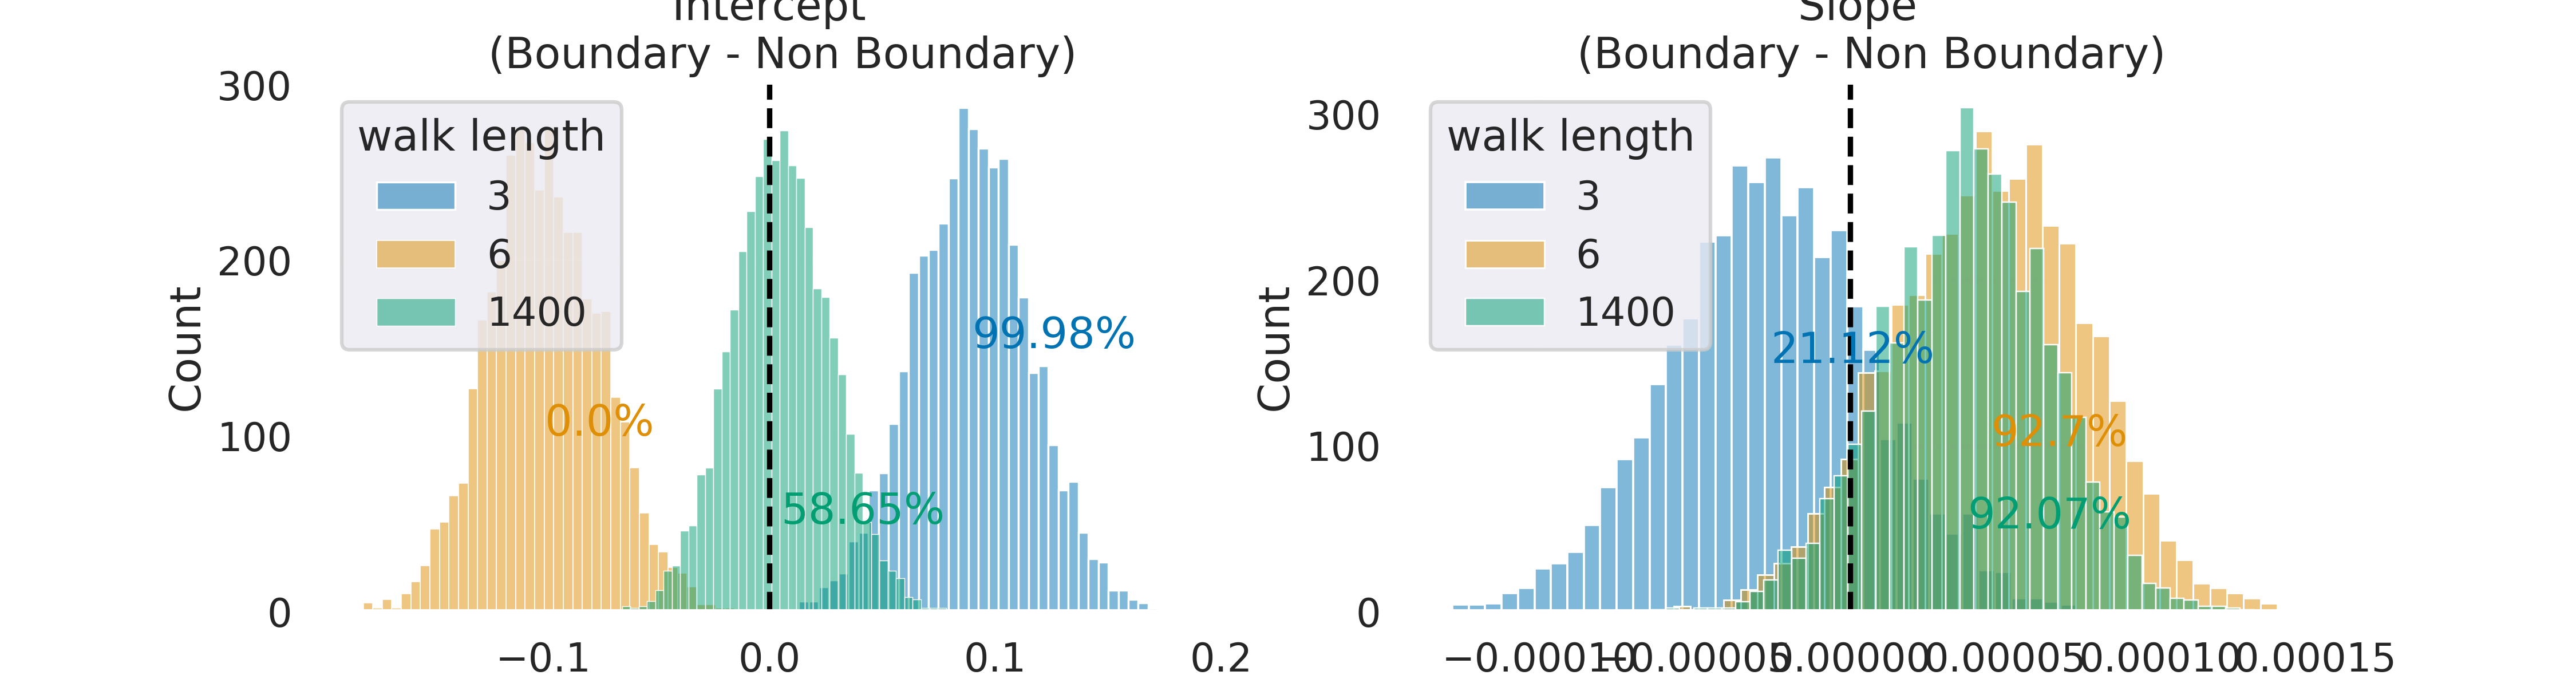
\includegraphics[width = \textwidth]{chapter_notebooks/chapter_2/figures/allblocks_lrmodel_trial_ppt_lag.png}
    \caption{Intercept (\textit{Left panel}) and Slope (\textit{Right panel}) differences of the linear model fit to all trials.}
    \label{fig:alltrial-lrmodel}
\end{figure}

As shown in figure \ref{fig:alltrial-lrmodel}, boundary and non boundary intercepts differed across walk lengths. This difference is likely due to randomly assigned response keys. The key metric of differences is the reduction in response times over time as measured by the slopes. As expected (from the SR model), walk lengths of 3 and 1399 lead to slower decrease in response times for boundary nodes than non boundary nodes (when transitioned to from another within cluster (non boundary) node). 

Interestingly, it appears that these slope differences are not meaningfully different between walk lengths of 6 and 1399. However, the findings reported in the main text (Figure \ref{fig:bayesmodel-firsttwoblocks}), it is likely that these differences were apparent earlier in the learning process for the walk length of 1399 than for walk length of 6. Conflicting results with the main text likely implies a need for a more complex model (such as a dual rate model \cite{mcdougle2015explicit, smith2006interacting, savalia2022leap}) which allows for a quick initial decrease in reaction times followed by a slow asymptote. Future modeling work should investigate the impact of walk lengths on different aspects of the learning process.

\section{Model Statistics}

\subsection*{Stats for comparisons between the RTs for the first two blocks}

\begin{table}[H]
    \centering
    \begin{tabular}{lrrrr}
        \toprule
         & mean & sd & hdi 2.5\% & hdi 97.5\% \\
        \midrule
        beta block[0.0] & -0.066 & 0.176 & -0.409 & 0.269 \\
        beta block[1.0] & -0.080 & 0.177 & -0.417 & 0.271 \\
        beta lag & 0.039 & 0.007 & 0.026 & 0.053 \\
        beta transition exp & -0.018 & 0.004 & -0.025 & -0.011 \\
        beta trial ntr[boundary, 0.0] & -0.555 & 0.024 & -0.602 & -0.508 \\
        beta trial ntr[boundary, 1.0] & -0.629 & 0.028 & -0.685 & -0.574 \\
        beta trial ntr[nonboundary, 0.0] & -0.596 & 0.023 & -0.639 & -0.548 \\
        beta trial ntr[nonboundary, 1.0] & -0.650 & 0.028 & -0.702 & -0.596 \\
        \bottomrule
        \end{tabular}        
        \caption{Posterior parameter statistics for model fit to walk length 3 data comparing the first two blocks}
        \label{tab:first-two-blocks-3}
\end{table}

\begin{table}[H]
    \centering
    \begin{tabular}{lrrrr}
        \toprule
         & mean & sd & hdi 2.5\% & hdi 97.5\% \\
        \midrule
        beta block[0.0] & 0.143 & 0.173 & -0.191 & 0.482 \\
        beta block[1.0] & 0.124 & 0.181 & -0.225 & 0.475 \\
        beta lag & 0.043 & 0.008 & 0.028 & 0.058 \\
        beta transition exp & -0.031 & 0.004 & -0.038 & -0.023 \\
        beta trial ntr[boundary, 0.0] & 0.252 & 0.033 & 0.190 & 0.319 \\
        beta trial ntr[boundary, 1.0] & 0.184 & 0.037 & 0.111 & 0.257 \\
        beta trial ntr[nonboundary, 0.0] & 0.316 & 0.033 & 0.252 & 0.383 \\
        beta trial ntr[nonboundary, 1.0] & 0.241 & 0.037 & 0.165 & 0.310 \\
        \bottomrule
    \end{tabular}
    \caption{Posterior parameter statistics for model fit to walk length 6 data comparing the first two blocks}
    \label{tab:first-two-blocks-6}
\end{table}

\begin{table}[H]
    \centering
    \begin{tabular}{lrrrr}
        \toprule
         & mean & sd & hdi 2.5\% & hdi 97.5\% \\
        \midrule
        beta block[0.0] & -0.043 & 0.172 & -0.378 & 0.294 \\
        beta block[1.0] & -0.076 & 0.177 & -0.427 & 0.267 \\
        beta lag & 0.066 & 0.007 & 0.053 & 0.080 \\
        beta transition exp & -0.010 & 0.003 & -0.016 & -0.005 \\
        beta trial ntr[nonboundary, 0.0] & -0.476 & 0.023 & -0.522 & -0.431 \\
        beta trial ntr[nonboundary, 1.0] & -0.635 & 0.027 & -0.688 & -0.581 \\
        beta trial ntr[boundary, 0.0] & -0.499 & 0.024 & -0.546 & -0.455 \\
        beta trial ntr[boundary, 1.0] & -0.602 & 0.027 & -0.655 & -0.548 \\
        \bottomrule
        \end{tabular}   
        \caption{Posterior parameter statistics for model fit to walk length 1399 data comparing the first two blocks}
        \label{tab:first-two-blocks-1399}    
\end{table}

\subsection*{Stats for comparisons between the RTs for the first and last blocks}

\begin{table}[H]
    \centering
    \begin{tabular}{lrrrr}
        \toprule
         & mean & sd & hdi 2.5\% & hdi 97.5\% \\
        \midrule
        beta block[0.0] & -0.070 & 0.173 & -0.392 & 0.274 \\
        beta block[6.0] & -0.100 & 0.172 & -0.431 & 0.236 \\
        beta lag & 0.029 & 0.006 & 0.017 & 0.041 \\
        beta transition exp & -0.007 & 0.002 & -0.010 & -0.003 \\
        beta trial ntr[boundary, 0.0] & -0.561 & 0.020 & -0.601 & -0.523 \\
        beta trial ntr[boundary, 6.0] & -0.704 & 0.037 & -0.778 & -0.634 \\
        beta trial ntr[nonboundary, 0.0] & -0.604 & 0.020 & -0.642 & -0.563 \\
        beta trial ntr[nonboundary, 6.0] & -0.730 & 0.039 & -0.808 & -0.656 \\
        \bottomrule
    \end{tabular}        
    \caption{Posterior parameter statistics for model fit to walk length 3 data comparing the first and the last blocks}
    \label{tab:first-last-blocks-3}    
\end{table}

\begin{table}[H]
    \centering
    \begin{tabular}{lrrrr}
        \toprule
         & mean & sd & hdi 2.5\% & hdi 97.5\% \\
        \midrule
        beta block[0.0] & -0.054 & 0.175 & -0.406 & 0.279 \\
        beta block[6.0] & -0.099 & 0.178 & -0.460 & 0.228 \\
        beta lag & 0.038 & 0.006 & 0.026 & 0.050 \\
        beta transition exp & -0.006 & 0.002 & -0.010 & -0.003 \\
        beta trial ntr[boundary, 0.0] & -0.538 & 0.019 & -0.574 & -0.501 \\
        beta trial ntr[boundary, 6.0] & -0.734 & 0.038 & -0.809 & -0.660 \\
        beta trial ntr[nonboundary, 0.0] & -0.528 & 0.020 & -0.568 & -0.489 \\
        beta trial ntr[nonboundary, 6.0] & -0.700 & 0.038 & -0.777 & -0.629 \\
        \bottomrule
    \end{tabular}
    \caption{Posterior parameter statistics for model fit to walk length 6 data comparing the first and the last blocks}
    \label{tab:first-last-blocks-6}    
    
\end{table}

\begin{table}[H]
    \centering
    \begin{tabular}{lrrrr}
        \toprule
         & mean & sd & hdi 2.5\% & hdi 97.5\% \\
        \midrule
        beta block[0.0] & -0.053 & 0.178 & -0.404 & 0.306 \\
        beta block[6.0] & -0.122 & 0.176 & -0.458 & 0.230 \\
        beta lag & 0.060 & 0.006 & 0.049 & 0.072 \\
        beta transition exp & -0.003 & 0.001 & -0.006 & -0.001 \\
        beta trial ntr[nonboundary, 0.0] & -0.515 & 0.019 & -0.553 & -0.478 \\
        beta trial ntr[nonboundary, 6.0] & -0.845 & 0.034 & -0.910 & -0.778 \\
        beta trial ntr[boundary, 0.0] & -0.538 & 0.020 & -0.576 & -0.499 \\
        beta trial ntr[boundary, 6.0] & -0.825 & 0.034 & -0.891 & -0.762 \\
        \bottomrule
    \end{tabular}        
    \caption{Posterior parameter statistics for model fit to walk length 1399 data comparing the first and the last blocks}
    \label{tab:first-last-blocks-1399}    
\end{table}


\subsection*{Parameter statistics for linear model including all trials}

\begin{table}[H]
    \centering
    \begin{tabular}{lrrrr}
        \toprule
         & mean & sd & hdi 2.5\% & hdi 97.5\% \\
        \midrule
        alpha ntr[3, boundary] & 0.466 & 0.138 & 0.215 & 0.760 \\
        alpha ntr[3, nonboundary] & 0.376 & 0.138 & 0.106 & 0.650 \\
        alpha ntr[6, boundary] & 0.440 & 0.138 & 0.166 & 0.699 \\
        alpha ntr[6, nonboundary] & 0.539 & 0.138 & 0.261 & 0.789 \\
        alpha ntr[1400, boundary] & 0.489 & 0.134 & 0.281 & 0.826 \\
        alpha ntr[1400, nonboundary] & 0.484 & 0.133 & 0.263 & 0.802 \\
        beta ntr[3, boundary] & -0.000 & 0.000 & -0.001 & -0.000 \\
        beta ntr[3, nonboundary] & -0.000 & 0.000 & -0.001 & -0.000 \\
        beta ntr[6, boundary] & -0.000 & 0.000 & -0.001 & -0.000 \\
        beta ntr[6, nonboundary] & -0.001 & 0.000 & -0.001 & -0.000 \\
        beta ntr[1400, boundary] & -0.001 & 0.000 & -0.001 & -0.001 \\
        beta ntr[1400, nonboundary] & -0.001 & 0.000 & -0.001 & -0.001 \\
        \bottomrule
    \end{tabular}        
    \caption{Parameter statistics for linear model fitting all trials. Parameter `alpha' is the intercept, and parameter `beta' is the slope of the linear model.}
    \label{tab:allblocks-trial-ppt-lag}         
\end{table}

\chapter{Chapter 3}

\begin{table}[H]
    \centering
    \caption{Bayesian SDT Model results for boundary nodes from experiment 3a. }
    \label{tab:exp3-bayesmodel-boundary-sdt}
    \begin{tabular}{lrrrr}
        \toprule
         & mean & sd & hdi 3\% & hdi 97\% \\
        \midrule
        accuracy exposure & -0.805 & 0.716 & -2.088 & 0.591 \\
        true old|structured & 4.088 & 0.332 & 3.472 & 4.711 \\
        true old|unstructured & 4.200 & 0.308 & 3.611 & 4.783 \\
        true old|condition sigma & 5.228 & 2.233 & 1.934 & 9.368 \\
        \bottomrule
        \end{tabular}        
\end{table}

\begin{table}[H]
    \centering
    \caption{Bayesian SDT Model results for non boundary nodes from experiment 3a. }
    \label{tab:exp3-bayesmodel-nonboundary-sdt}
    \begin{tabular}{lrrrr}
        \toprule
         & mean & sd & hdi 3\% & hdi 97\% \\
        \midrule
        accuracy exposure & -1.347 & 0.715 & -2.665 & -0.020 \\
        true old|structured & 3.885 & 0.269 & 3.398 & 4.406 \\
        true old|unstructured & 4.593 & 0.299 & 4.017 & 5.122 \\
        true old|condition sigma & 5.156 & 2.002 & 2.010 & 8.873 \\
        \bottomrule
        \end{tabular}
        
\end{table}

\begin{table}[H]
    \centering
    \caption{Drift diffusion model parameters for experiment 3a.}
    \label{tab:exp3-ddm-params}
    \begin{tabular}{lrrrrrrrrr}
        \toprule
        parameter, condition, block & mean & sd & hdi 3\% & hdi 97\% \\
        \midrule
        a structured, 0 & 1.259 & 0.022 & 1.220 & 1.300 \\
        a structured, 1 & 1.144 & 0.021 & 1.104 & 1.183 \\
        a structured, 2 & 1.121 & 0.021 & 1.081 & 1.159 \\
        a unstructured, 0 & 1.306 & 0.023 & 1.263 & 1.349 \\
        a unstructured, 1 & 1.237 & 0.025 & 1.193 & 1.284 \\
        a unstructured, 2 & 1.149 & 0.023 & 1.107 & 1.191 \\
        v boundary, structured, 0 & 0.385 & 0.092 & 0.202 & 0.546 \\
        v boundary, structured, 1 & 0.476 & 0.096 & 0.294 & 0.653 \\
        v boundary, structured, 2 & 0.688 & 0.097 & 0.506 & 0.873 \\
        v boundary, unstructured, 0 & 0.554 & 0.108 & 0.357 & 0.753 \\
        v boundary, unstructured, 1 & 0.761 & 0.101 & 0.565 & 0.944 \\
        v boundary, unstructured, 2 & 0.830 & 0.106 & 0.637 & 1.029 \\
        v new, structured, 0 & -0.733 & 0.062 & -0.848 & -0.618 \\
        v new, structured, 1 & -1.124 & 0.077 & -1.267 & -0.980 \\
        v new, structured, 2 & -1.011 & 0.075 & -1.159 & -0.879 \\
        v new, unstructured, 0 & -0.872 & 0.062 & -0.986 & -0.754 \\
        v new, unstructured, 1 & -1.414 & 0.081 & -1.560 & -1.259 \\
        v new, unstructured, 2 & -1.267 & 0.079 & -1.408 & -1.112 \\
        v nonboundary, structured, 0 & 0.236 & 0.069 & 0.102 & 0.362 \\
        v nonboundary, structured, 1 & 0.468 & 0.081 & 0.326 & 0.631 \\
        v nonboundary, structured, 2 & 0.570 & 0.084 & 0.411 & 0.730 \\
        v nonboundary, unstructured, 0 & 0.619 & 0.079 & 0.471 & 0.768 \\
        v nonboundary, unstructured, 1 & 0.830 & 0.092 & 0.663 & 1.005 \\
        v nonboundary, unstructured, 2 & 0.927 & 0.097 & 0.749 & 1.114 \\
        z 0 & 0.499 & 0.010 & 0.481 & 0.517 \\
        z 1 & 0.505 & 0.010 & 0.485 & 0.523 \\
        z 2 & 0.489 & 0.010 & 0.470 & 0.507 \\
        \bottomrule
        \end{tabular}
        
\end{table}

\begin{table}[H]
    \centering
    \caption{Bayesian model results for Experiment 3b.}
    \label{lab:exp3-bayesmodel-stats}
    \begin{tabular}{lrrrr}
        \toprule
        True Distance, Condition & mean & sd & hdi 3\% & hdi 97\% \\
        \midrule
        1, structured & 0.222 & 0.191 & -0.155 & 0.562 \\
        1, unstructured & 0.096 & 0.224 & -0.338 & 0.496 \\
        2, structured & -0.026 & 0.205 & -0.401 & 0.358 \\
        2, unstructured & 0.113 & 0.234 & -0.329 & 0.543 \\
        3, structured & -0.320 & 0.280 & -0.857 & 0.184 \\
        3, unstructured & -0.505 & 0.337 & -1.137 & 0.106 \\
        \bottomrule
        \end{tabular}
        
\end{table}

\chapter{Chapter 4}
\section{Model Statistics}
\begin{table}[H]
    \centering
    \caption{Bayesian model statistics for experiment 4a}
    \label{tab:exp4-bayes-model-results}
    \begin{tabular}{lrrrr}
        \toprule
        Num Features, Condition & mean & sd & hdi 3\% & hdi 97\% \\
        \midrule
        1.0, structured & 0.324 & 0.308 & -0.240 & 0.927 \\
        1.0, unstructured & 0.236 & 0.304 & -0.300 & 0.832 \\
        2.0, structured & 0.661 & 0.309 & 0.077 & 1.253 \\
        2.0, unstructured & 0.031 & 0.304 & -0.508 & 0.621 \\
        3.0, structured & 0.563 & 0.311 & -0.004 & 1.152 \\
        3.0, unstructured & 0.189 & 0.302 & -0.350 & 0.753 \\
        4.0, structured & 0.564 & 0.306 & -0.017 & 1.138 \\
        4.0, unstructured & 0.126 & 0.303 & -0.444 & 0.684 \\
        \bottomrule
        \end{tabular}
        
\end{table}

\begin{table}[H]
    \centering
    \caption{Bayesian model statistics for experiment 4b.}
    \label{tab:exp5-bayes-model-results}
    \begin{tabular}{lrrrr}
        \toprule
         Num Features, Category Determinant & mean & sd & hdi 3\% & hdi 97\% \\
        \midrule
        1.0, A & 1.005 & 0.372 & 0.303 & 1.693 \\
        1.0, B & -1.529 & 0.438 & -2.361 & -0.713 \\
        2.0, A & 1.338 & 0.378 & 0.620 & 2.036 \\
        2.0, B & -1.803 & 0.443 & -2.638 & -0.977 \\
        3.0, A & 1.299 & 0.378 & 0.551 & 1.987 \\
        3.0, B & -1.709 & 0.439 & -2.508 & -0.848 \\
        4.0, A & 1.687 & 0.385 & 0.977 & 2.435 \\
        4.0, B & -1.706 & 0.442 & -2.596 & -0.948 \\
        \bottomrule
        \end{tabular}
        
\end{table}

\section{Feature Differences}
Experiment 3b provides an indication that categorization (regardless of if it is dependent on temporal consistency) depends on the importance of each visual feature of the stimuli. At test, participants categorized the previously seen stimulus by matching its feature to the two on-screen options. On each test trial, the on-screen options differ from each other in one to four features such that for the `category' option all the category diagnostic features (those that remained temporally consistent during exposure) remained the same as the test stimulus. For the `non category' option, the features that were not category diagnostic (those that frequently changed during exposure) remained the same as the test stimulus. Thus, in order to categorize based on category diagnostic features, participants must \textit{ignore} the different valued non-category diagnostic features in the category option. Furthermore, participants must use the different category diagnostic feature in the non-category option to decide to not pick that option. 

A logistic regression model was fit where each feature was coded as whether it was identical in the non-category option (relative to the test stimulus). If a feature changed in the non category option, (hence was identical in the category option), it was coded as '1' otherwise it was coded as '0'. Fitting this model thus provided a measure of the weights a participant placed on that feature to select the category option. Figure 

\begin{figure}[H]
    \centering
    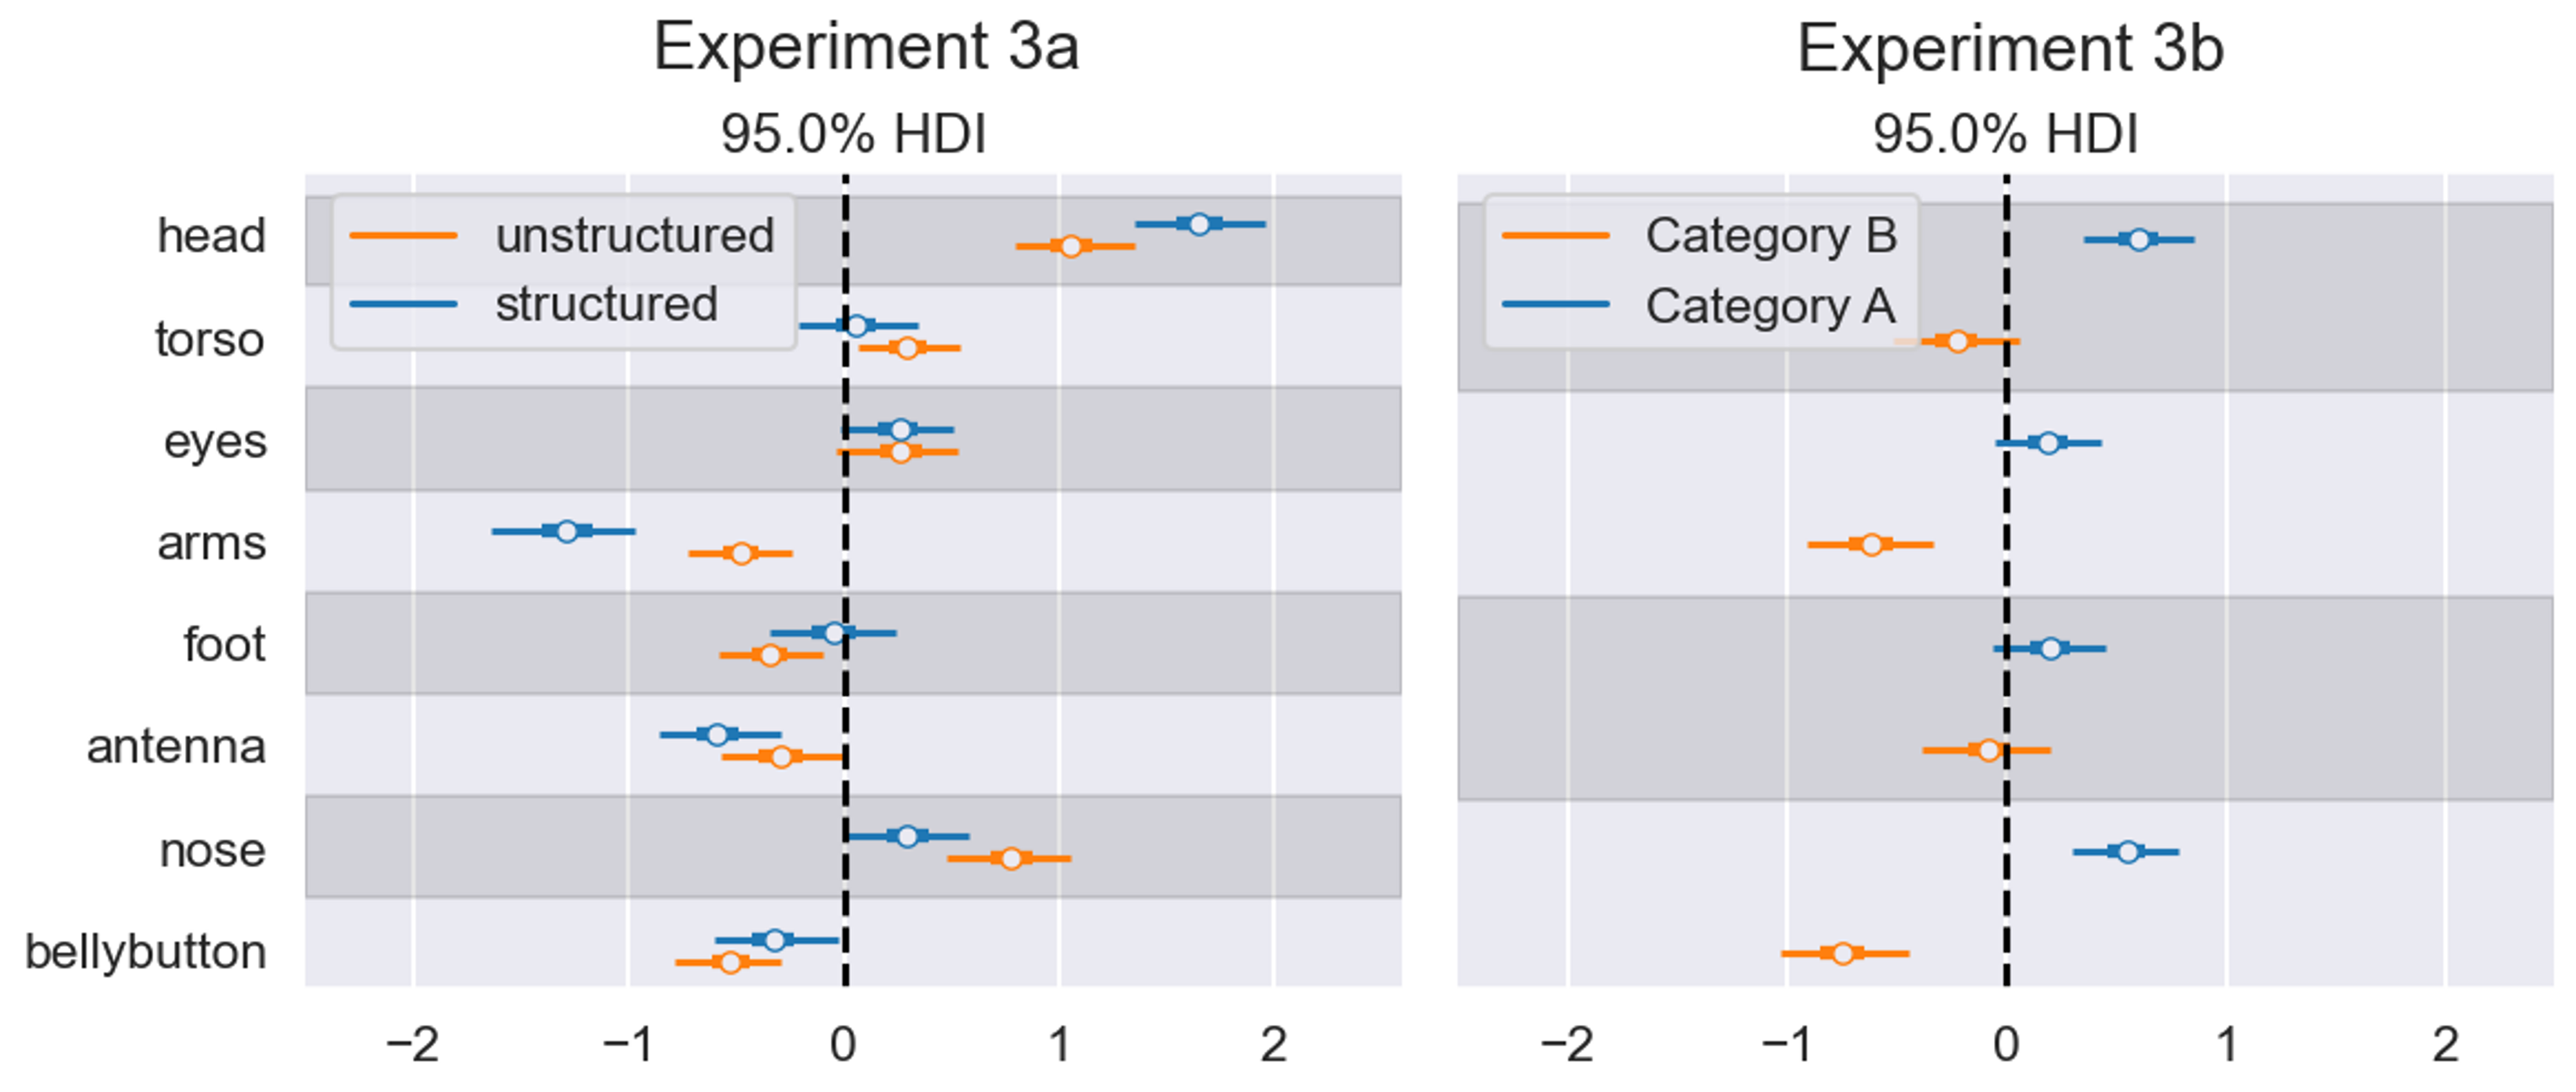
\includegraphics[width = \textwidth]{chapter_notebooks/chapter_4/figures/feat_importances.png}
    \caption{Relative weights placed by participants to categorize test stimuli. Values above 0 indicate features that are category diagnostic (i.e. remained consistent during exposure) are chosen more often to categorize whereas values below 0 indicate features that are category non-diagnostic (i.e. changed frequently) are used to categorize.}
    \label{fig:feat-importances}
\end{figure}

As seen in figure \ref{fig:feat-importances}, some features are grouped together for being temporally consistent whereas some features are grouped together for being temporally inconsistent. Interestingly, this is true even in the unstructured case. Regardless of the temporal exposure, participants will group aliens together if they have the same head color or nose shape. On average, features that were chosen to be category diagnostic for Category A participants in experiment 3b (head, eyes, foot, and nose), were inherently grouped together for sharing feature values. Whereas features that were chosen to be category diagnostic for Category B participants in experiment 3b (torso, arms, antenna, bellybutton) were inherently grouped together if the did \textit{not} share feature values. While this analysis does not address covariances among features, it provides a possible explanation for patterns in Experiment 3b -- visual features carry different weights in categorization. Based on their weights, attention may be drawn to them either for being temporally consistent or for being temporally inconsistent. Future modeling will aim to assess whether attention weights modulate 

\interlinepenalty=10000  % prevent split bibliography entries

\bibliography{references}
\bibliographystyle{umassthesis}

	
% \printbibliography

\end{document}

%% 
%% Copyright (C) 2019 by Daniel A. Weiss <daniel.weiss.led at gmail.com>
%% 
%% This work may be distributed and/or modified under the
%% conditions of the LaTeX Project Public License (LPPL), either
%% version 1.3c of this license or (at your option) any later
%% version.  The latest version of this license is in the file:
%% 
%% http://www.latex-project.org/lppl.txt
%% 
%% Users may freely modify these files without permission, as long as the
%% copyright line and this statement are maintained intact.
%% 
%% This work is not endorsed by, affiliated with, or probably even known
%% by, the American Psychological Association.
%% 
%% This work is "maintained" (as per LPPL maintenance status) by
%% Daniel A. Weiss.
%% 
%% This work consists of the file  apa7.dtx
%% and the derived files           apa7.ins,
%%                                 apa7.cls,
%%                                 apa7.pdf,
%%                                 README,
%%                                 APA7american.txt,
%%                                 APA7british.txt,
%%                                 APA7dutch.txt,
%%                                 APA7english.txt,
%%                                 APA7german.txt,
%%                                 APA7ngerman.txt,
%%                                 APA7greek.txt,
%%                                 APA7czech.txt,
%%                                 APA7turkish.txt,
%%                                 APA7endfloat.cfg,
%%                                 Figure1.pdf,
%%                                 shortsample.tex,
%%                                 longsample.tex, and
%%                                 bibliography.bib.
%% 
%%
%%
%% This is file `./samples/shortsample.tex',
%% generated with the docstrip utility.
%%
%% The original source files were:
%%
%% apa7.dtx  (with options: `shortsample')
%% ----------------------------------------------------------------------
%% 
%% apa7 - A LaTeX class for formatting documents in compliance with the
%% American Psychological Association's Publication Manual, 7th edition
%% 
%% Copyright (C) 2019 by Daniel A. Weiss <daniel.weiss.led at gmail.com>
%% 
%% This work may be distributed and/or modified under the
%% conditions of the LaTeX Project Public License (LPPL), either
%% version 1.3c of this license or (at your option) any later
%% version.  The latest version of this license is in the file:
%% 
%% http://www.latex-project.org/lppl.txt
%% 
%% Users may freely modify these files without permission, as long as the
%% copyright line and this statement are maintained intact.
%% 
%% This work is not endorsed by, affiliated with, or probably even known
%% by, the American Psychological Association.
%% 
%% ----------------------------------------------------------------------